\documentclass[12pt, letterpaper]{article}
\usepackage{float}
\usepackage{parskip}
\usepackage{graphicx}
\usepackage{setspace}
\usepackage{appendix}
\usepackage{amsmath}
\usepackage{amssymb}
\usepackage{geometry}
\usepackage{csvsimple}
\usepackage{indentfirst}
\usepackage{subcaption}
\usepackage{anyfontsize}
\usepackage[utf8]{inputenc}
\usepackage[american]{babel}
\usepackage[babel]{csquotes}
\usepackage[	style=phys,
				articletitle=false,
				backend=bibtex,
				biblabel=brackets,
				chaptertitle=false,
				pageranges=false]{biblatex}
				
\usepackage{hyperref}
\hypersetup{
	colorlinks=true,
	linkcolor=blue,
	filecolor=magenta,
	urlcolor=cyan,
}

\addbibresource{physics-ia.bib}
\defbibheading{center}{%
	\phantomsection
	\section*{\centering\normalfont\refname}
	\pdfbookmark{\refname}{References}
}
\bibliography{physics-ia}

\geometry{letterpaper, portrait, margin=1in}
\graphicspath{{../imgs/}}

\newcommand{\sorta}[1]{`#1'}
\newcommand{\poses}[1]{#1's}

\title{The Optimal Strength-Retaining Hole Pattern for Sheet Material}
\author{Tynan Purdy}
\date{May 2019}

\begin{document}
\nocite{*}
\large
\doublespace{}
\parindent=0.5in

{\fontsize{12}{14.4}
  {\singlespace
    \pagenumbering{gobble}
    \maketitle
    \begin{center}
    002129-0004 \\
    \vspace{4mm}
    IB Physics HL IA \\
    \vspace{4mm}
    Words: 1604  \\ % words
    \end{center}
  }
}	

\newpage
\pagenumbering{arabic}

%TC:break Abstract
\begin{abstract}
One of the greatest challenges of structural engineering is to reduce the weight of a system without compromising its strength. Hole patterns are a go-to solution to make parts lighter and maintain the majority of their rigidity. The problem is, what hole pattern is best? With many 2D tessellation patterns to choose from, it can be difficult to determine the optimal pattern to use. This investigation will simulate stresses on test sheet parts with a variety of polygon hole patterns to determine which shape maintains the highest strength in an array of scenarios. 

Words: 94 % words

\end{abstract}
%TC:break _main_

\newpage
\tableofcontents
\newpage

\section{Background}
\label{sec:background}

Sheet metal is one of the most commonly used materials in engineering, but especially finds its place in the field of robotics. Sheet metal provides a stiff, structural component while taking little space and weight. Robotics frequently requires complicated geometry in small volumes. Sometimes sheet metal can be used as a light structural material instead of solid or tube extrusion. In the FIRST Robotics Competition (FRC), teams use sheet metal to make custom gearboxes, gussets, base-plates, even entire drive-trains. For all of these applications, applying a lightening hole pattern is a great way to reduce weight while maintaining an acceptable durability and stiffness. As seen in Figure \ref{fig:frc1}, not every team uses the same pattern.

\begin{figure}[H]
	\centering
	\caption{FRC Examples of Hole Patterns}
	\label{fig:frc1}
	\begin{subfigure}[t]{.64\linewidth}
		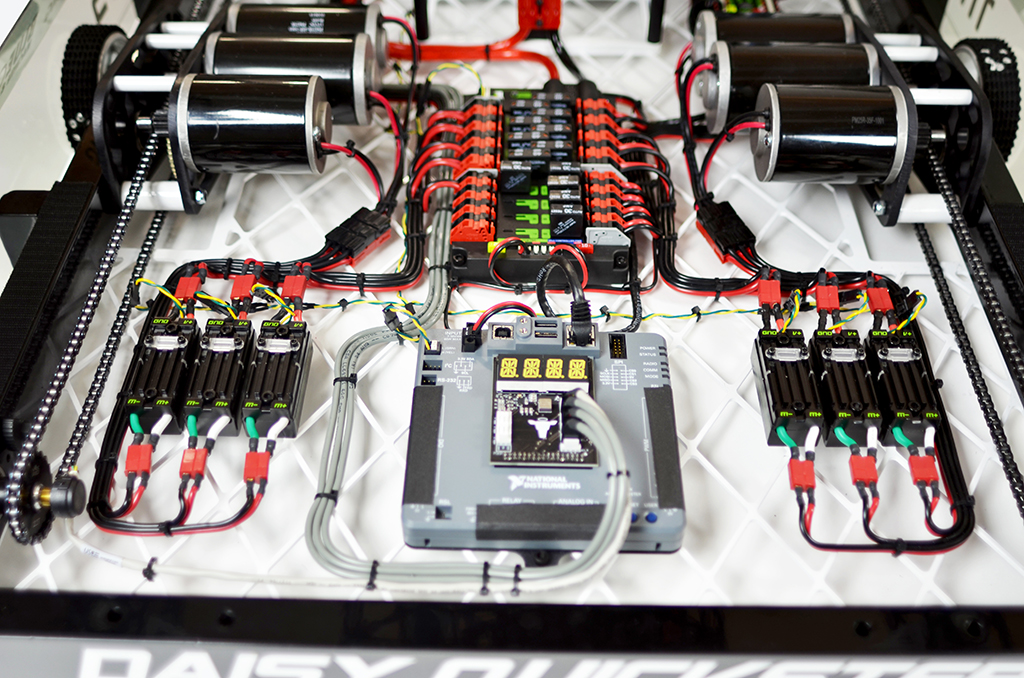
\includegraphics[width=\linewidth]{frc-ex1}
		\caption{FRC robot (team 1538) with a rectangular diamond hole pattern}
	\end{subfigure}
	\begin{subfigure}[t]{.35\linewidth}
		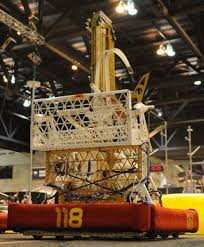
\includegraphics[width=\linewidth]{frc-ex2}
		\caption{FRC robot made almost entirely out of sheet metal (team 118) with a triangular hole pattern}
	\end{subfigure}
\end{figure}

\subsection{Statics}
\label{sec:statics}

Statics is an area of physics thoroughly used in engineering, and particularly in the area of solid mechanics and structural engineering. For this investigation of a solid object under various loads and forces, solid mechanics provides a paradigm of study. Statics analyzes torque and force moments applied to a system, which is exactly what these simulations will do. 

\begin{singlespace}
\begin{equation}
	\label{eq:force}
	|\vec{M_O}| = \vec{F} \cdot \vec{r} = \vec{\tau}
\end{equation}
\begin{small}
	\begin{itemize}
	\item[] $|\vec{M_O}| =$ vector force moment
	\item[] $\vec{F} =$ vector force applied
	\item[] $\vec{r} =$ perpendicular distance to axis of rotation
	\end{itemize}
\end{small}
\end{singlespace}

For each simulation, displacement  between $t_i$ and $t_f$ is recorded. Displacement is the vector change in position between initial position and final position, generically described as $\vec r_i - \vec r_f = \vec d$. In the SolidWorks Simulation, the models for force moments and displacement are far more accurate than the simplified models described. 

\subsection{Solid Mechanics}
\label{sec:solid-mechanics}

The field of solid mechanics analyzes the deformations of a solid under system changes. Deformation is the change ($\Delta$) between the rest shape and the final shape. These changes can include changes in forces, temperature, phase changes and other internal or external changes \autocite{chou_elasticity:_1992}. A variety of models have been developed to describe different types of deformations of solids, and their properties:

\begin{itemize}
\item Stress: The restoring force over a specific cross-sectional area
\item Strain: The response of a system to an applied stress
\item Plasticity: The degree to which an object can deform
\item Elasticity: The degree to which an object can return to rest shape after deformation
\end{itemize}

Stress is the force exerted by a material, against the external force, to return to rest shape, divided by the cross sectional area. For this investigation, the stress and strain model will be used to describe the characterize the simulated deformations in tension, compression and torsion. The model is an extension of Hooke's law, which describes the behavior of a spring. This similarity makes sense because all materials have some degree of elasticity, and therefore, can behave as a spring. 

\begin{singlespace}
\begin{equation}
	\label{eq:stress}
	\sigma_x \equiv \lim_{\Delta A \rightarrow 0} \frac{\Delta N}{\Delta A}
\end{equation}
\begin{small}
\begin{itemize}
\item[] $\sigma_x =$ stress
\item[] $\Delta N =$ fraction of normal force $N$
\item[] $\Delta A =$ cross-sectional area element
\end{itemize}
\end{small}
\end{singlespace}


\begin{singlespace}
\begin{equation}
	\label{eq:strain}
	\varepsilon_x \equiv \frac{\sigma_x}{E} + \alpha \Delta T
\end{equation}
\begin{small}
\begin{itemize}
\item[] $\varepsilon_x =$ strain
\item[] $\sigma_x =$ stress
\item[] $E =$ modulus of elasticity
\item[] $\alpha =$ temperature coefficient
\item[] $\Delta T =$ change of temperature
\end{itemize}
\end{small}
\end{singlespace}

Equations \ref{eq:stress} and \ref{eq:strain} are basic models of stress and strain. The simulations will be run using the SolidWorks Simulation add-in, which uses the Von Mises model for stress and strain by default (Equations \ref{eq:von-mises-stress} and \ref{eq:von-mises-strain}). The derivation of the Von Mises model is beyond the scope of this investigation, however it is an industry standard and is suitable for use in simulation. 

\begin{equation}
	\label{eq:von-mises-stress}
	\sigma_{ij} = \frac{1}{3} \delta_{ij} \sigma_{kk} + \sigma^\prime_{ij}
\end{equation}

\begin{equation}
	\label{eq:von-mises-strain}
	\varepsilon_{ij} = \frac{1}{3} \delta_{ij} \varepsilon_{kk} + \varepsilon^\prime_{ij}
\end{equation}

\section{Simulation}
\label{sec:simulation}

\subsection{Variables}
\label{sec:variables}

To keep the stress analysis of each part fair, certain properties were controlled for every part. 

\begin{itemize}
\item All parts have the dimensions of 1000mm x 1000mm x 5mm
\item All parts are set to the material 6061 Aluminum Alloy
\item All parts have a mass of 2.525kg, within $\pm2.5\%$ error (except the solid test part)
\item All parts have a 10mm perimeter with no holes
\item All polygon holes have a 10mm wide edge
\item An equal force will be applied to each part for each test
\end{itemize}

\begin{figure}[H]
	\centering
	\label{fig:6061ss}
	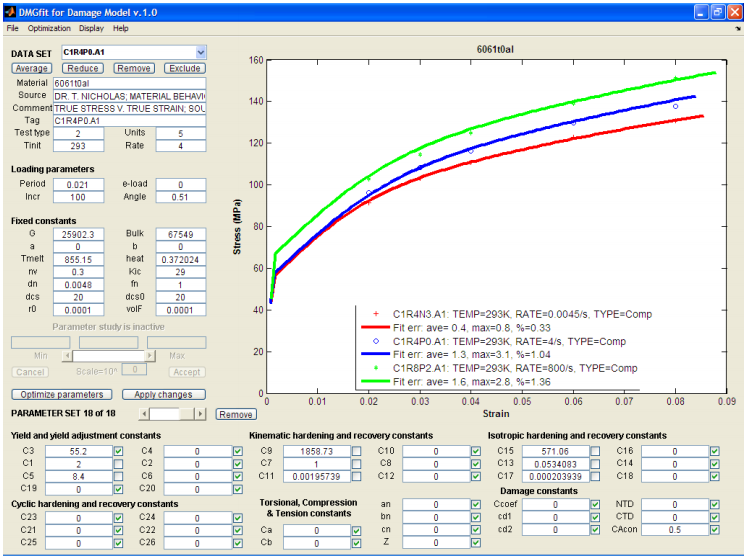
\includegraphics[width=.8\linewidth]{6061ss}
	\caption{Stress vs. Strain graph of 6061 T0 Aluminum Alloy\autocite{noauthor_ssc_nodate}}
\end{figure}

Above is the stress vs strain graph of the alloy used in all of the test parts. It shows the duration of strain for which the material behaves as a Hooke's law dictates, where the relationship is linear, and at what point permanent deformation will occur. 

Each part is not exactly 2.5kg because the skill in SolidWorks and time required to reach that target are beyond the scope of this investigation and the researcher. 2.5kg was chosen as the target mass because it was the approximate mass of the \sorta{square-pattern} part. The 10mm perimeter was included to ensure equal mass where forces will be applied in the various simulations, and that the parts would have a closed perimeter. 

Variables that will change based on the shape used, and be recorded, are as follows:

\begin{itemize}
\item Hole Area
\item Part Surface Area
\item Number of holes
\end{itemize}

A total of 6 different patterns will be tested in simulated stress tests (Figure \ref{fig:parts}).

\begin{enumerate}
\item Filled (control)
\item Square
\item Square Diamond
\item Hex
\item Hex Diamond
\item Triangle
\end{enumerate}

The \sorta{filled} pattern is a solid sheet. It is used as a reference test as well as a data point to show stress properties when no holes are used. It should be noted that not all holes have the same area since hole patterns that do not match the shape of the part will not fit an integer number of shapes, and some shapes will be \sorta{cut off}. The vertices of incomplete shapes are not identical to the vertices of whole holes. The inconsistent vertices may have an effect on the results of the investigation. The surface area of each part is the 2D surface area of the flat sheet. Note the artifact in the bottom left corner of the triangle patterned part. An area with a width wider than 10mm occurred because an edge and the perimeter are overlapped. There is also a horizontal edge across the entire width of the part near the bottom edge of the part, which can potentially affect the relative strength of that area. 

\begin{figure}[H]
	\caption{Test Parts}
	\label{fig:parts}
	\begin{subfigure}[b]{.3\linewidth}
		
\includegraphics[width=\linewidth]{filled}
		\caption{Filled}
	\end{subfigure}
	\begin{subfigure}[b]{.3\linewidth}
		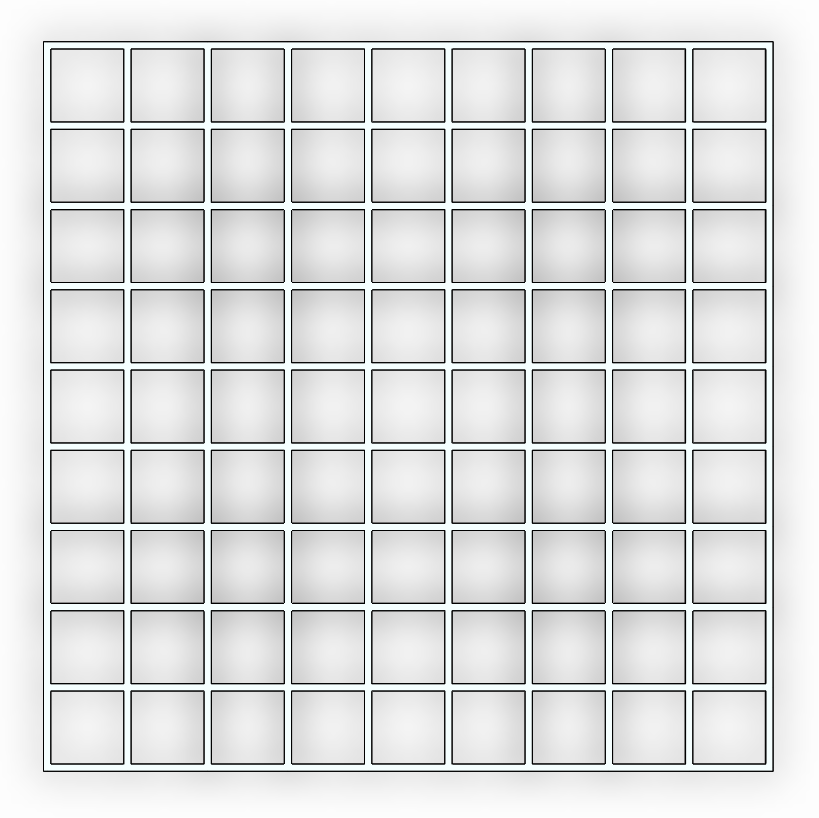
\includegraphics[width=\linewidth]{square}
		\caption{Square}
	\end{subfigure}
	\begin{subfigure}[b]{.3\linewidth}
		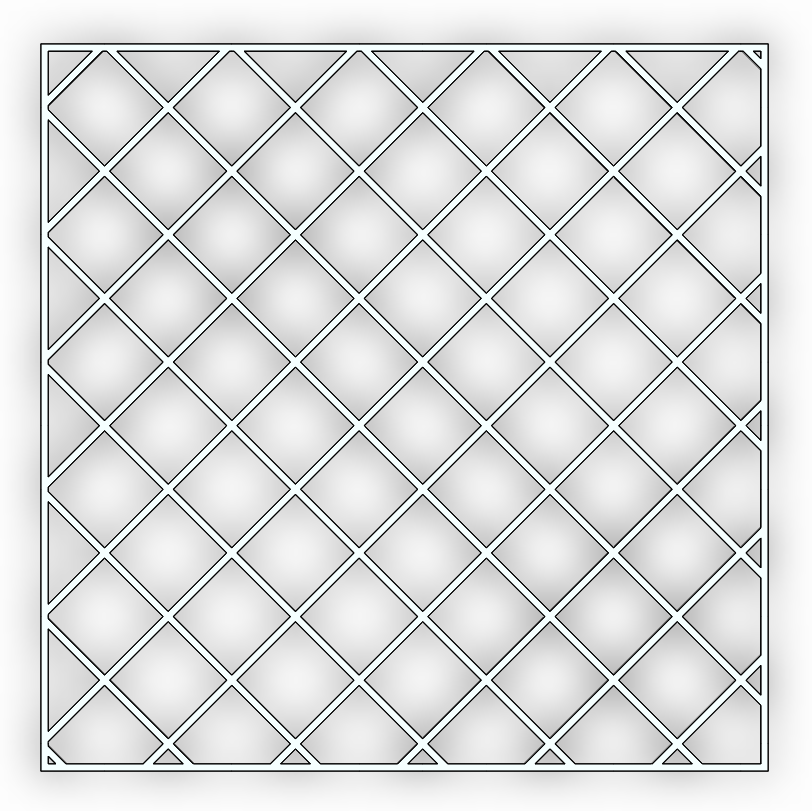
\includegraphics[width=\linewidth]{square-diamond}
		\caption{Square Diamond}
	\end{subfigure}
	\begin{subfigure}[b]{.3\linewidth}
		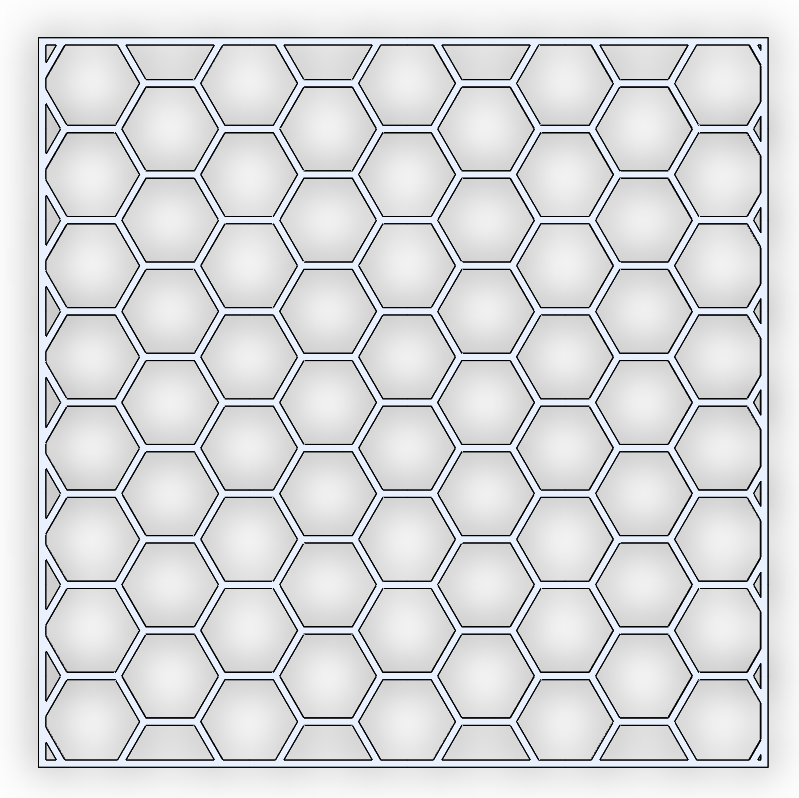
\includegraphics[width=\linewidth]{hex}
		\caption{Hex}
	\end{subfigure}
	\begin{subfigure}[b]{.3\linewidth}
		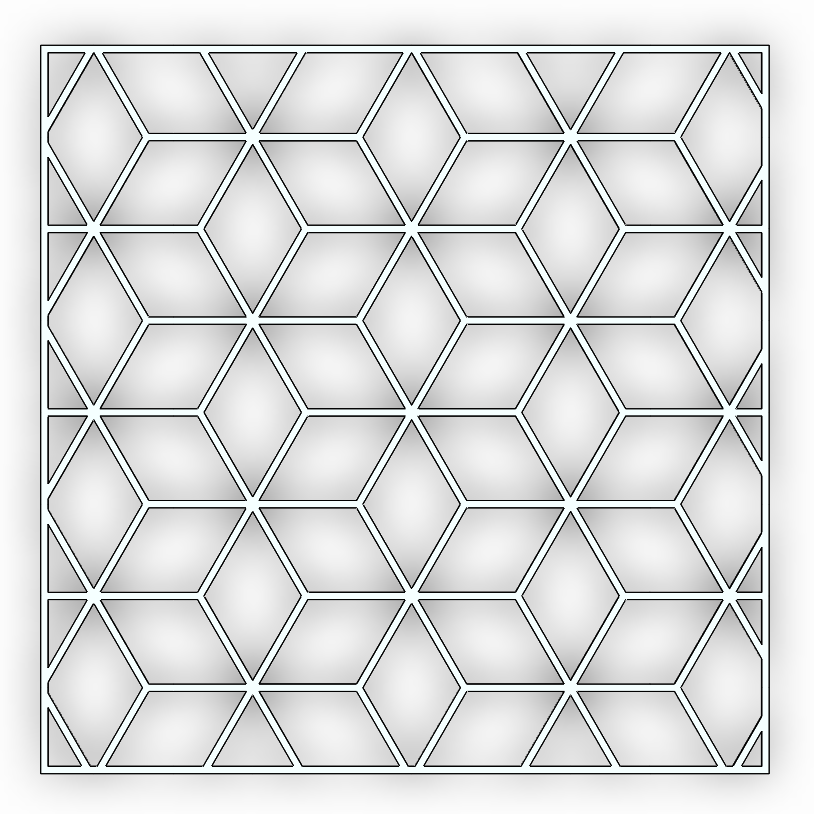
\includegraphics[width=\linewidth]{hex-diamond}
		\caption{Hex Diamond}
	\end{subfigure}
	\begin{subfigure}[b]{.3\linewidth}
		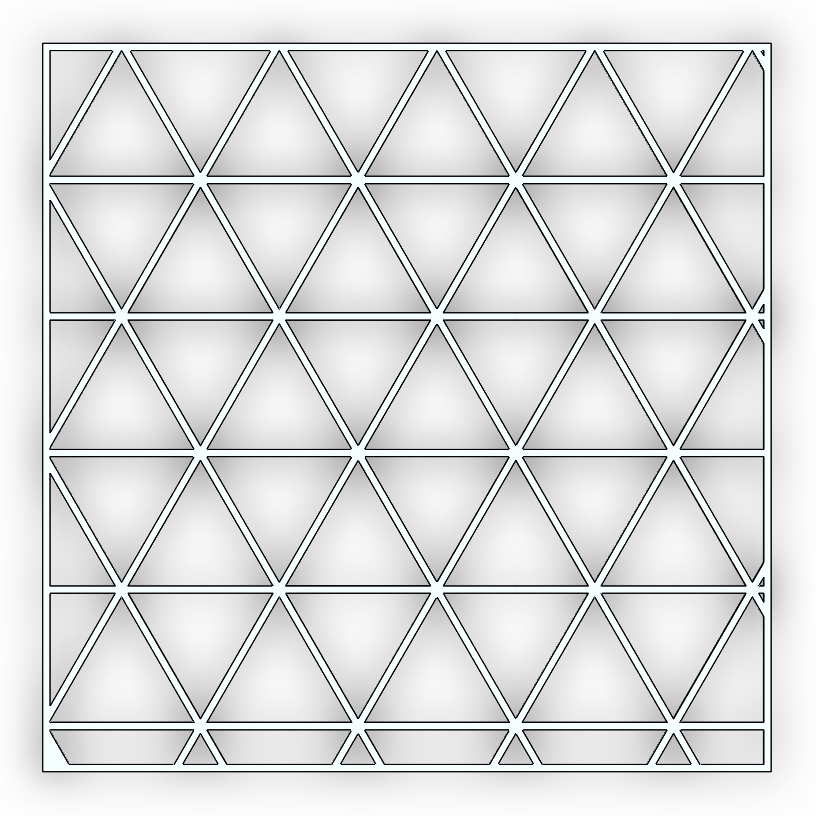
\includegraphics[width=\linewidth]{triangle}
		\caption{Triangle}
	\end{subfigure}
	\begin{subfigure}[b]{\linewidth}
	\begingroup
	\setlength{\tabcolsep}{10pt} % Default value: 6pt
	\renewcommand{\arraystretch}{1.5} % Default value: 1
		\begin{tabular}{ | c | c | c | c | c | }\hline
			Pattern 			& Mass (kg) 	& Surface Area (m$^2$)	& Max Hole Area (cm$^2$) 	& $n$ Holes 	\\\hline
			Filled				& 13.50 		& 1.000 						& 0			 					& 0			\\\hline
			Square			& 2.565 		& 0.190 						& 100.00		 					& 81			\\\hline
			Square Diamond	& 2.545 		& 0.188 						& 129.37	 						& 62.77		\\\hline
			Hex				& 2.506 		& 0.186 						& 114.55	 						& 71.06		\\\hline
			Hex Diamond		& 2.497 		& 0.185 						& 155.38	 						& 52.45		\\\hline
			Triangle			& 2.500 		& 0.185						& 170.65				 			& 47.76		\\\hline
		\end{tabular}
		\caption{Part Properties}
	\endgroup
	\end{subfigure}
\end{figure}

\newpage
\subsection{Procedure}
\label{sec:procedure}

A series of applied-load simulations will be performed on each of the 6 test parts. 

\begin{enumerate}
\item Linear Tension
\item Linear Compression
\item Torsion
\end{enumerate}

The same input parameters will be used in each simulation, with different directions of force (see Figure \ref{fig:sim-loads}). 

\begin{enumerate}
\item Fixed geometry includes one side face of the sheet (Figure \ref{fig:settings-fixed})
\item Force of 100N is applied to the face or edge opposite to the fixed face (Figure \ref{fig:sim-loads})
\item Mesh node size is 20mm$^2$ (Figure \ref{fig:settings-mesh})
\end{enumerate}

\begin{figure}[H]
	\centering
	\label{fig:sim-settings}
	\caption{Simulation Parameters}
	\begin{subfigure}[t]{.6\linewidth}
		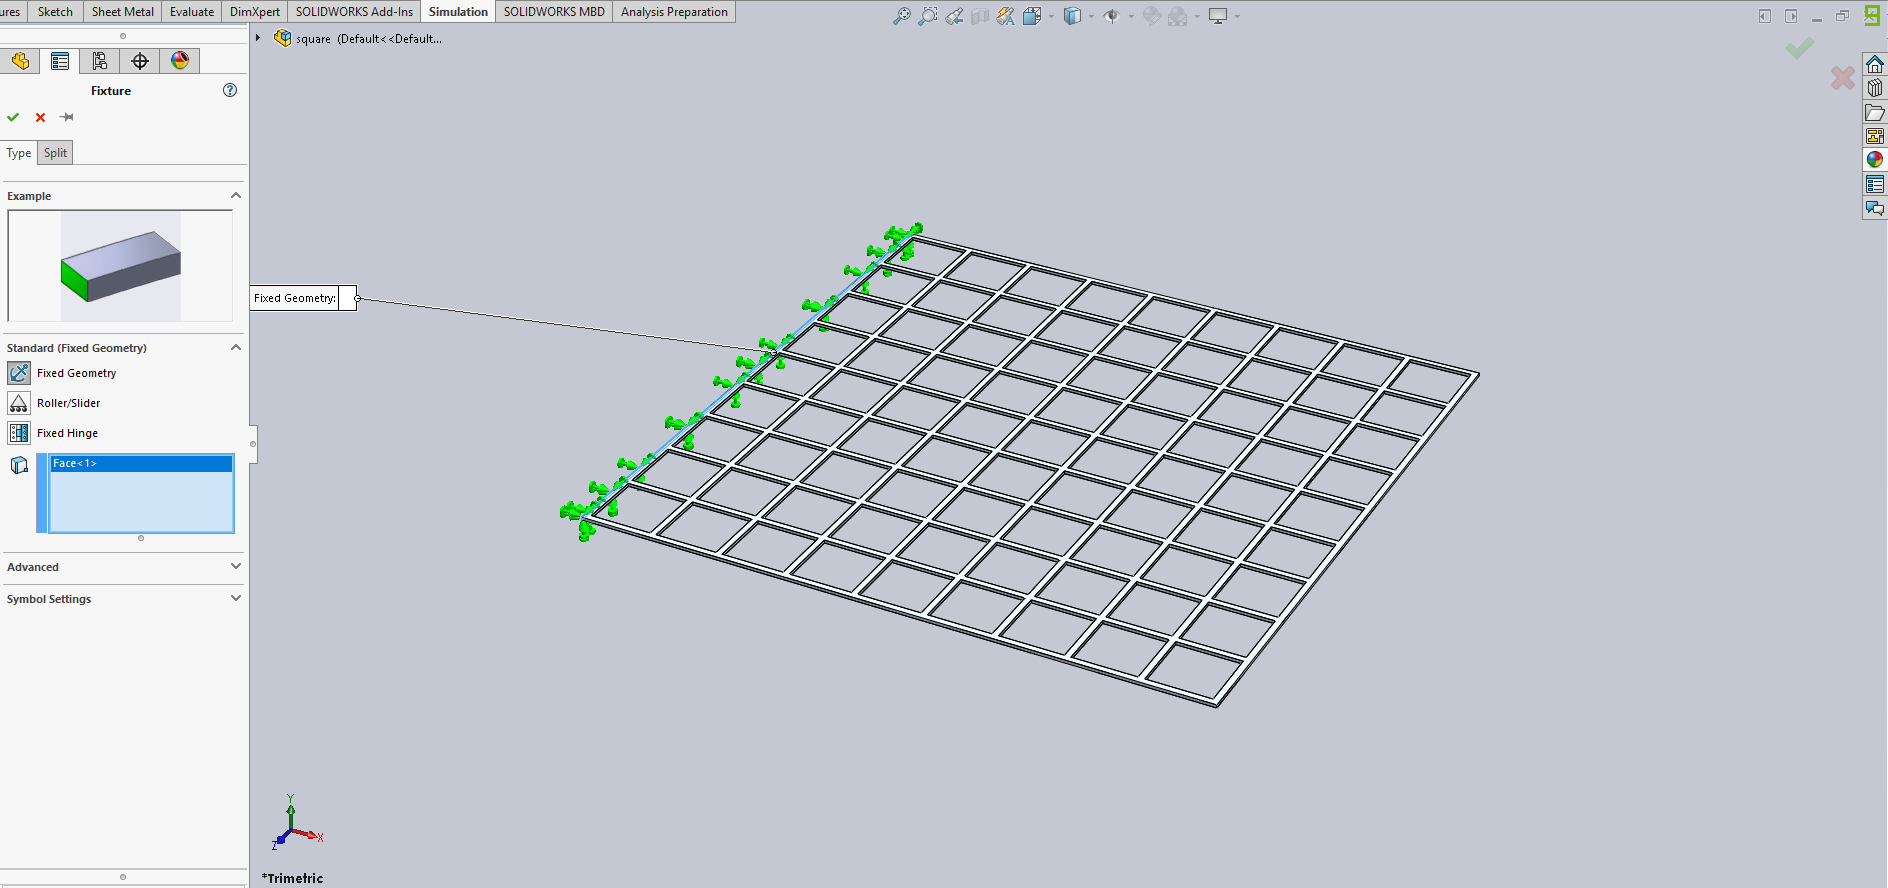
\includegraphics[width=\linewidth]{./procedure/fixed-geometry}
		\caption{Fixed geometry}
		\label{fig:settings-fixed}
	\end{subfigure}
	\begin{subfigure}[t]{.3\linewidth}
		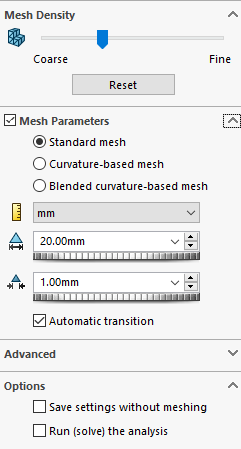
\includegraphics[width=\linewidth]{./procedure/mesh}
		\caption{Mesh size}
		\label{fig:settings-mesh}
	\end{subfigure}
\end{figure}

For linear tension, the force is applied on the face opposite to the fixed face and directed normal to the face and outward. 
For linear compression, the force is applied on the face opposite to the fixed face and directed normal to the face and inward.
For torsion, the force is applied on the top corner edge of the face opposite to the fixed face.

\begin{figure}[H]
	\centering
	\caption{Applied Loads}
	\label{fig:sim-loads}
	\begin{subfigure}[t]{.8\linewidth}
		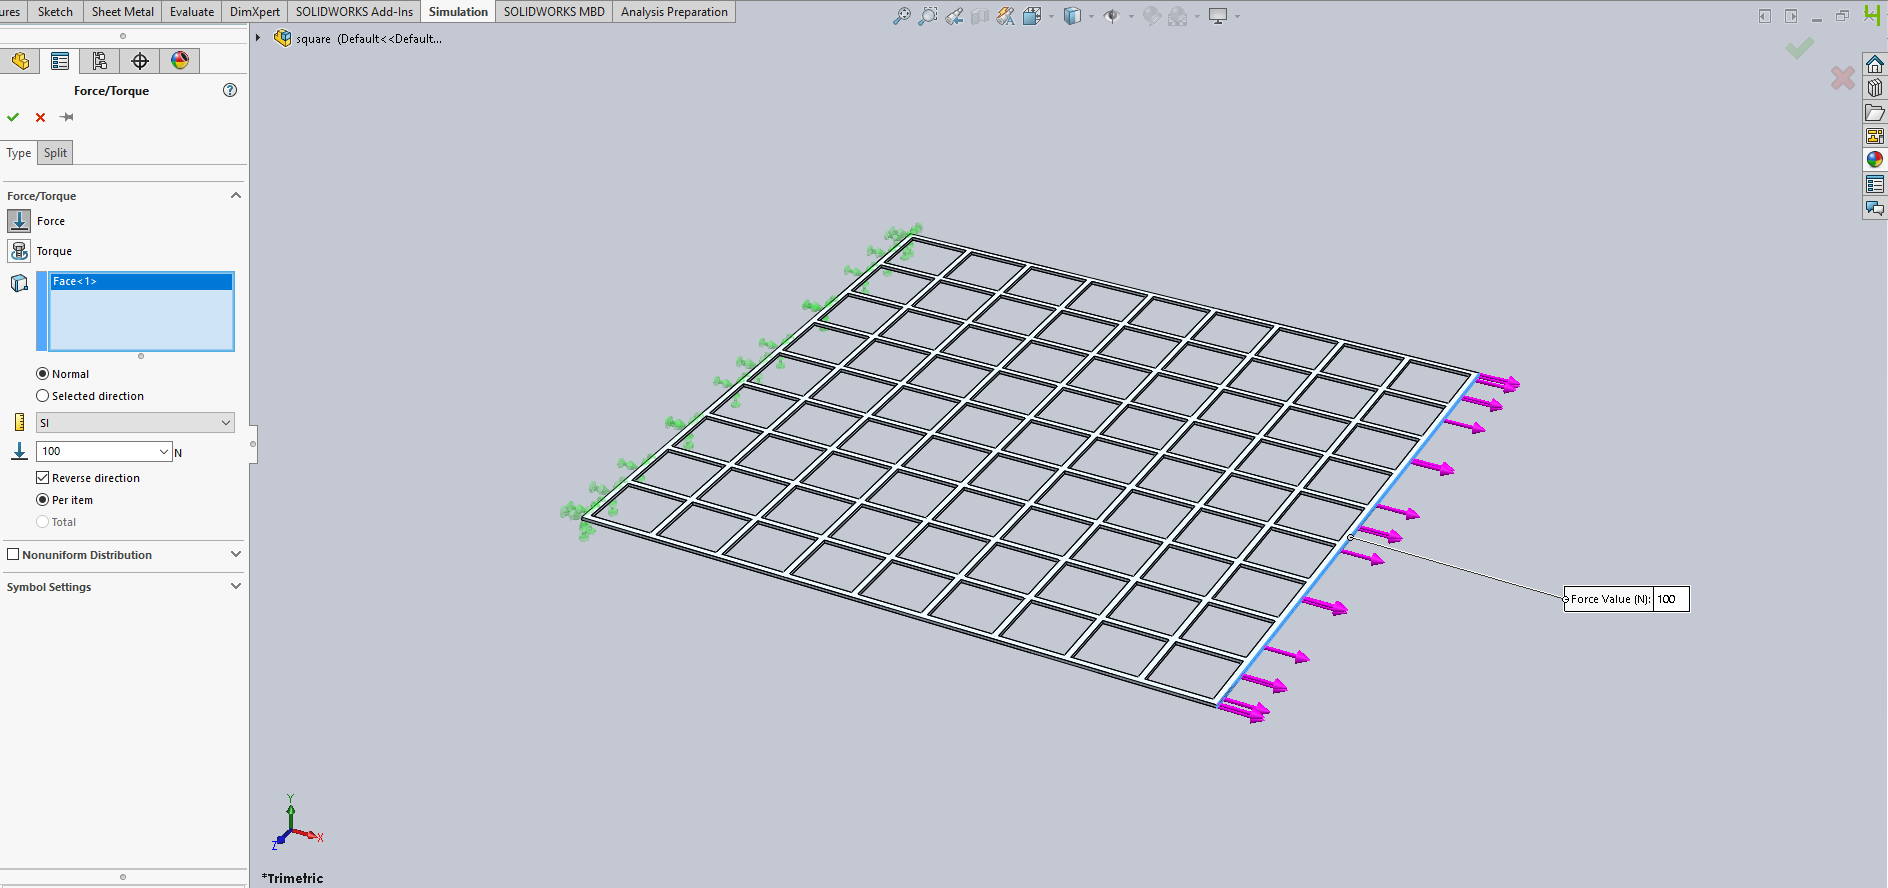
\includegraphics[width=\linewidth]{./procedure/tension-force}
		\caption{Tension Force}
	\end{subfigure}
	\begin{subfigure}[t]{.8\linewidth}
		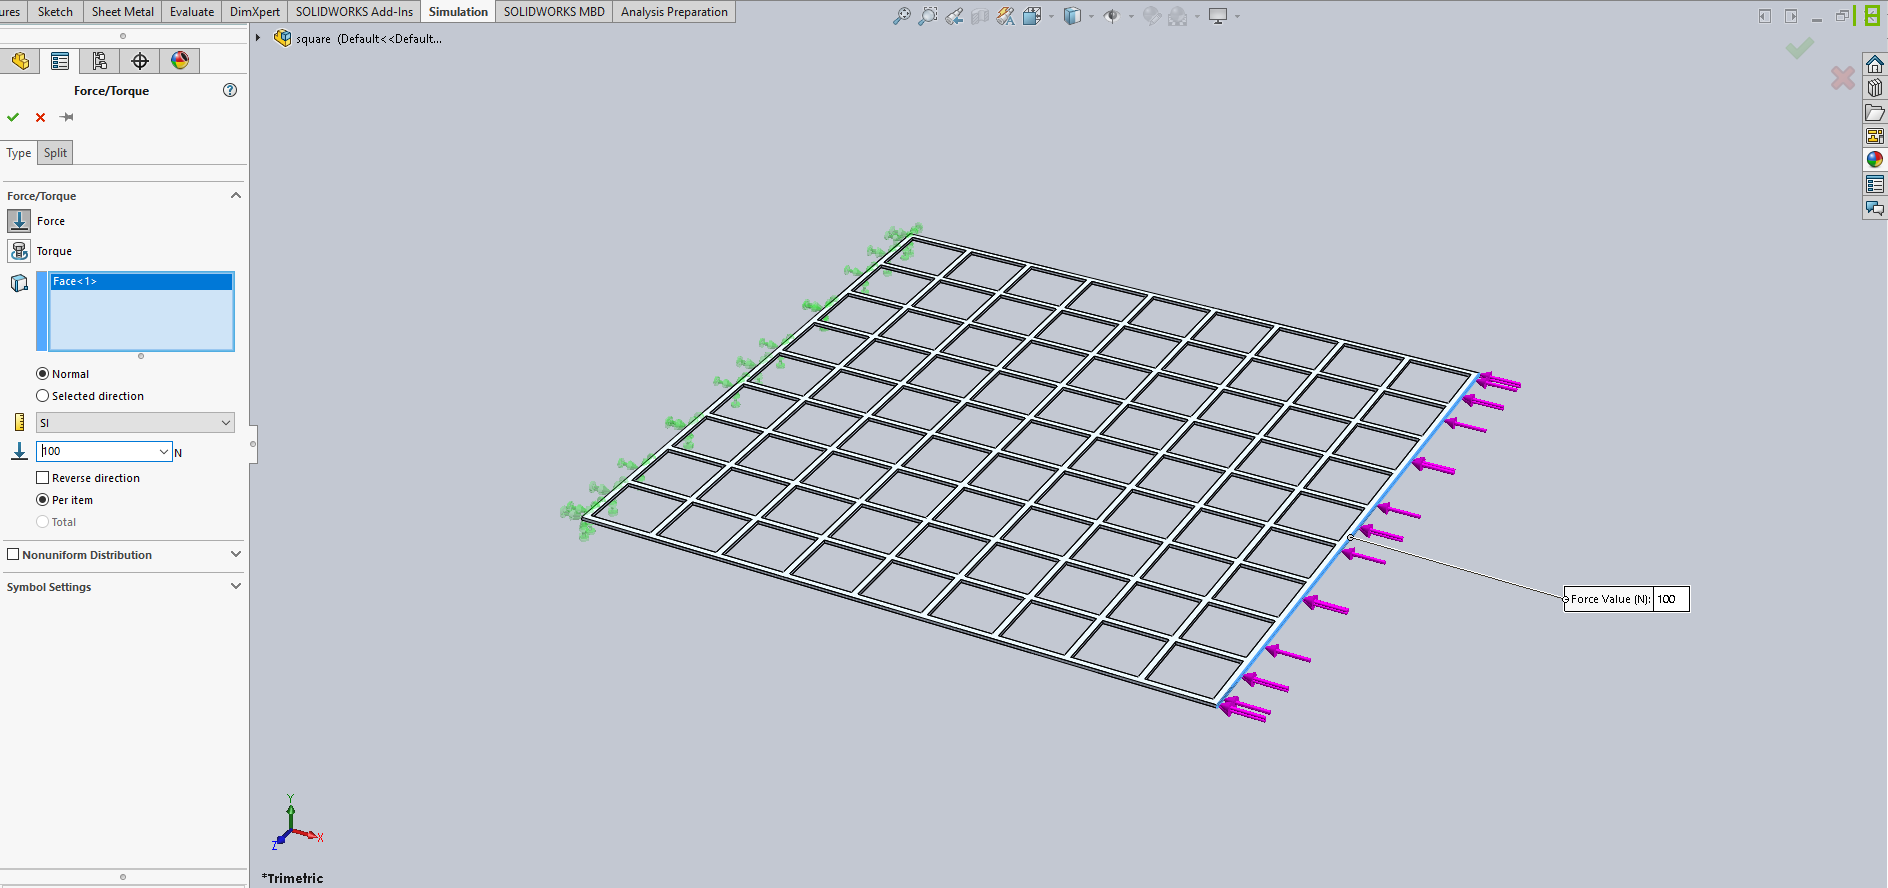
\includegraphics[width=\linewidth]{./procedure/compression-force}
		\caption{Compression Force}
	\end{subfigure}
	\begin{subfigure}[t]{.8\linewidth}
		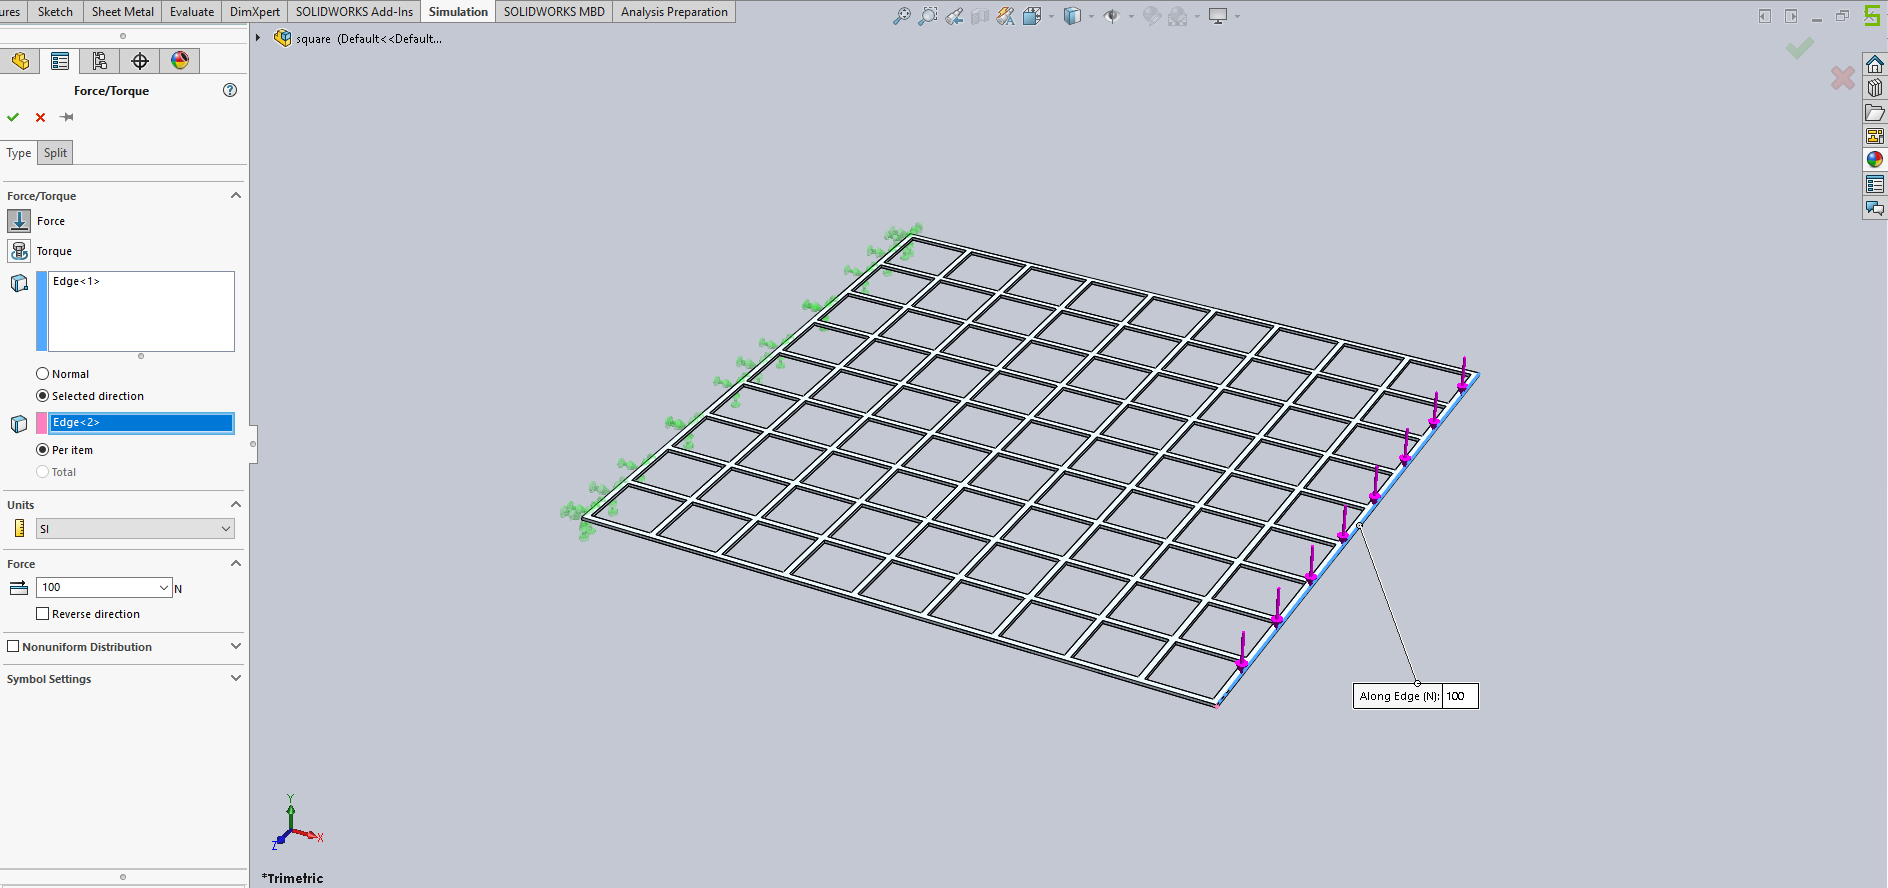
\includegraphics[width=\linewidth]{./procedure/torsion-force}
		\caption{Torsion Force}
	\end{subfigure}
\end{figure}

The simulation is run after fixed geometry, forces, and mesh size are configured. 
Every simulation is documented with three graphs of the final state color coded for von Mises stress, equivalent strain and URES displacement. An animation of the load force acting on the part is saved, as well as a .csv file of the final stress, strain, and displacement at each mesh node along the front plane. The .csv export settings are displayed in Figure \ref{fig:sim-data}. All graphs are displayed in Appendices \ref{ap:te}, \ref{ap:c}, and \ref{ap:to}. A link to .cvs files and .avi animation files is located in Appendix \ref{ap:data}. 

\begin{figure}[H]
	\centering
	\caption{Data Export}
	\label{fig:sim-data}
	\begin{subfigure}[t]{.3\linewidth}
		\caption{Stress .csv export}
		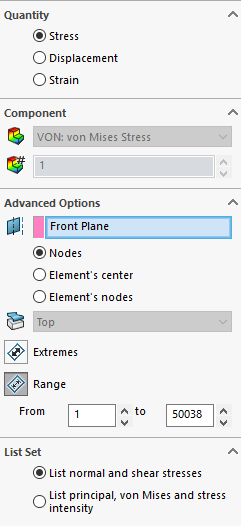
\includegraphics[width=\linewidth]{./procedure/stress-list}
	\end{subfigure}
	\begin{subfigure}[t]{.3\linewidth}
		\caption{Strain .csv export}
		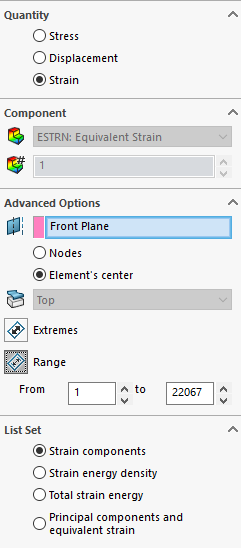
\includegraphics[width=\linewidth]{./procedure/strain-list}
	\end{subfigure}
	\begin{subfigure}[t]{.3\linewidth}
		\caption{Displacement .csv export}
		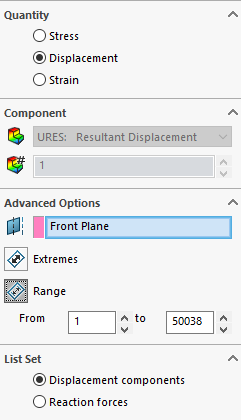
\includegraphics[width=\linewidth]{./procedure/displacement-list}
	\end{subfigure}
\end{figure}

\subsection{Results}
\label{sec:results}

The table in Figure \ref{fig:max} shows the maximum value of stress, strain, and displacement in each test for each part. 

\begin{figure}[H]
	\centering
	\caption{Maximum values reached for displacement, stress, and strain, per test and part}
	\label{fig:max}
	\begin{subfigure}[b]{0.8\linewidth}
	\label{tab:tension}
	\csvautotabular{../data/max-tension.csv}
	\caption{Maximums in tension}
	\end{subfigure}
	\begin{subfigure}[b]{0.8\linewidth}
	\label{tab:compression}
	\csvautotabular{../data/max-compression.csv}
	\caption{Maximums in compression}
	\end{subfigure}
	\begin{subfigure}[b]{0.8\linewidth}
	\label{tab:torsion}
	\csvautotabular{../data/max-torsion.csv}
	\caption{Maximums in torsion}
	\end{subfigure}
\end{figure}

As expected, the filled test part suffered the least amount of deformation in every test. Worth noting, however, is that it consistently had more strain than the parts with hole patterns, and less stress. 
Of the experimental parts, the triangle part showed the least deformation in all three tests. Looking at its graph of displacement in tension, Appendix \ref{ap:t-te-d}, the pattern itself shows almost no deformation. The deforming was localized to the edge of the part, where the force was applied. While triangle pattern deforms the least, it has higher stress and strain than the hex and square diamond patterns in tension and compression.
Hex diamond experiences the most deformation and strain in all tests, and is only exceeded in stress by square diamond. 


\section{Analysis}
\label{sec:analysis}

The results show low deformation from the triangle pattern. This is not unexpected, as the triangle is the only regular euclidean polygon with all acute internal angles. Acute internal angles allows the shape to support it self when external stress is applied (Appendix \ref{ap:t-c-vm}), rather than collapsing, as the other shapes did (Appendix \ref{ap:sd-c-vm}). Obtuse internal angles are prone to open wider under load (Appendix \ref{ap:h-c-vm}), straining the vertices of the holes instead of using the force to strengthen the shape. 

Appendix \ref{ap:s-te-es} demonstrates an interesting property. The strain from linear load is concentrated on edges parallel to the force, while little to no strain occurs in the edges perpendicular to the force. Shapes with edges out of alignment with the load will distribute the components of the force as a vector. The distributing behavior is best exhibited by Appendix \ref{ap:h-te-vm}, where the vertex closest to the tension force pulls on its neighboring vertices, a recursive process that is repeated in each hole. 

\section{Conclusion}
\label{sec:conclusion}

To return to the question of which hole pattern best preserves strength in a sheet part under load, the answer depends on the desired effect. The triangle pattern deforms the least, providing an extremely rigid part despite its weight. Peak stress and strain may be high, but that is mainly because the stress is localized and not allowed to spread throughout the part. On the other hand, the hex pattern diffuses stress and strain, reducing the overall damage to the part, but allows substantial deformation. 

For rigid applications, such as structural elements or metal parts, a triangular hole pattern has proven to be the best at withstanding deformation under load. For flexible components, such as rubber or silicon, a hexagon pattern will distribute forces and stresses the most, of the tested patterns. 

SolidWorks' simulation tools can be immensely valuable in the design process. Producing empirical data to choose design elements removes hours of testing, making safe and effective design more accessible and affordable. Practicing and learning the techniques in this investigation will be an advantage for my future engineering education and work. The conclusions of the investigation will aid many FRC teams that design lightened sheet metal parts. Of the two FRC examples in Figure \ref{fig:frc1}, it appears team 118 chose the right pattern. 

\newpage
\printbibliography{}

\newpage
\appendix
\addtocontents{toc}{\protect\setcounter{tocdepth}{1}}
\appendixpage
\addappheadtotoc
\listoffigures


\newpage
\begin{singlespace}
\section{Tension Test Graphs}
\label{ap:te}



\subsection{Tension Stress Graphs}
\label{ap:te-vm}


\subsubsection{Filled Tension Stress}
\label{ap:f-te-vm}
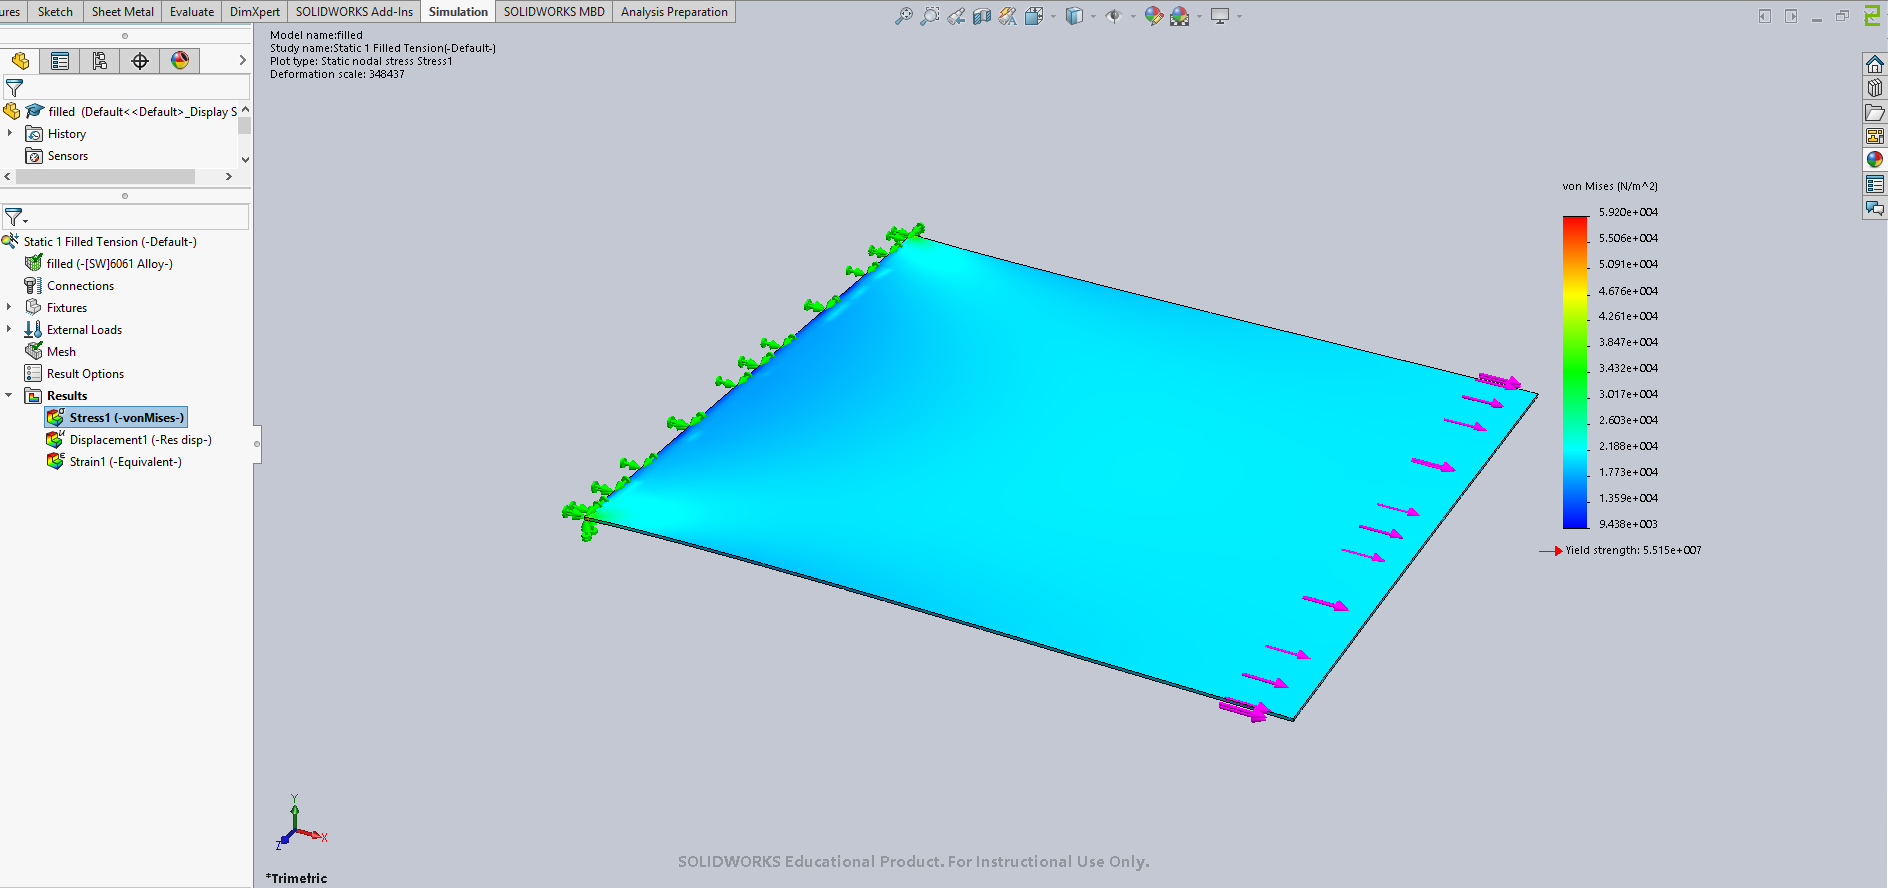
\includegraphics[width=0.8\linewidth]{./graphs/tension/filled-tension-stress}

\subsubsection{Square Tension Stress}
\label{ap:s-te-vm}
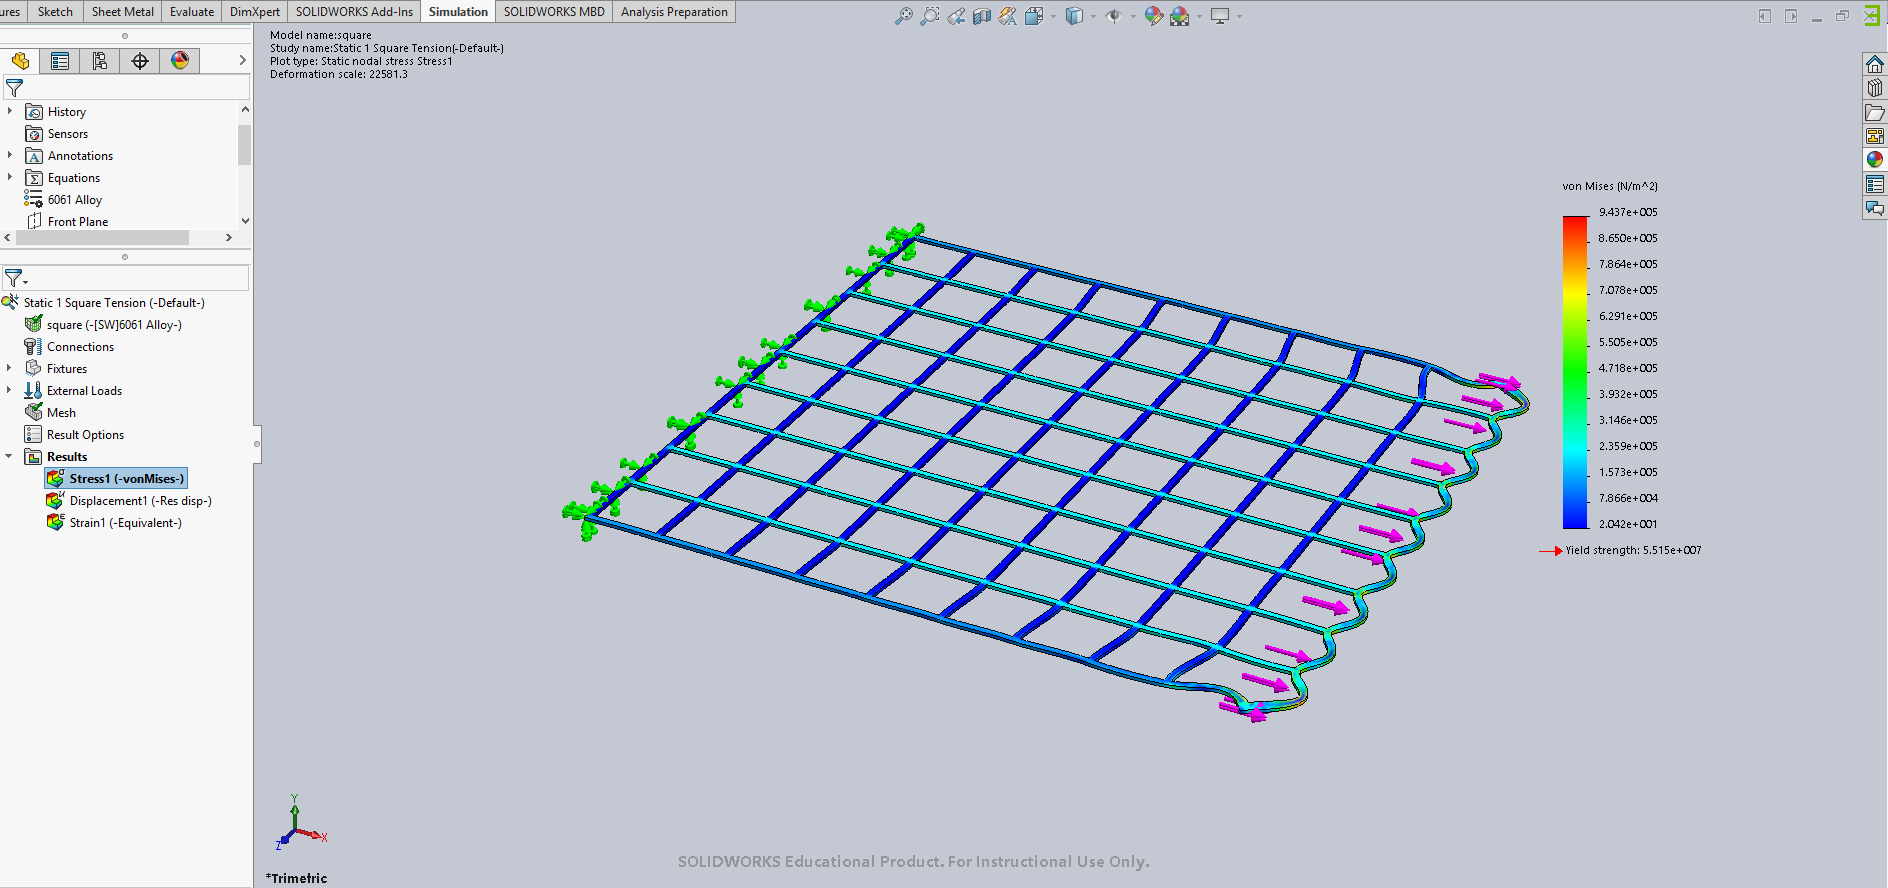
\includegraphics[width=0.8\linewidth]{./graphs/tension/square-tension-stress}

\subsubsection{Square Diamond Tension Stress}
\label{ap:sd-te-vm}
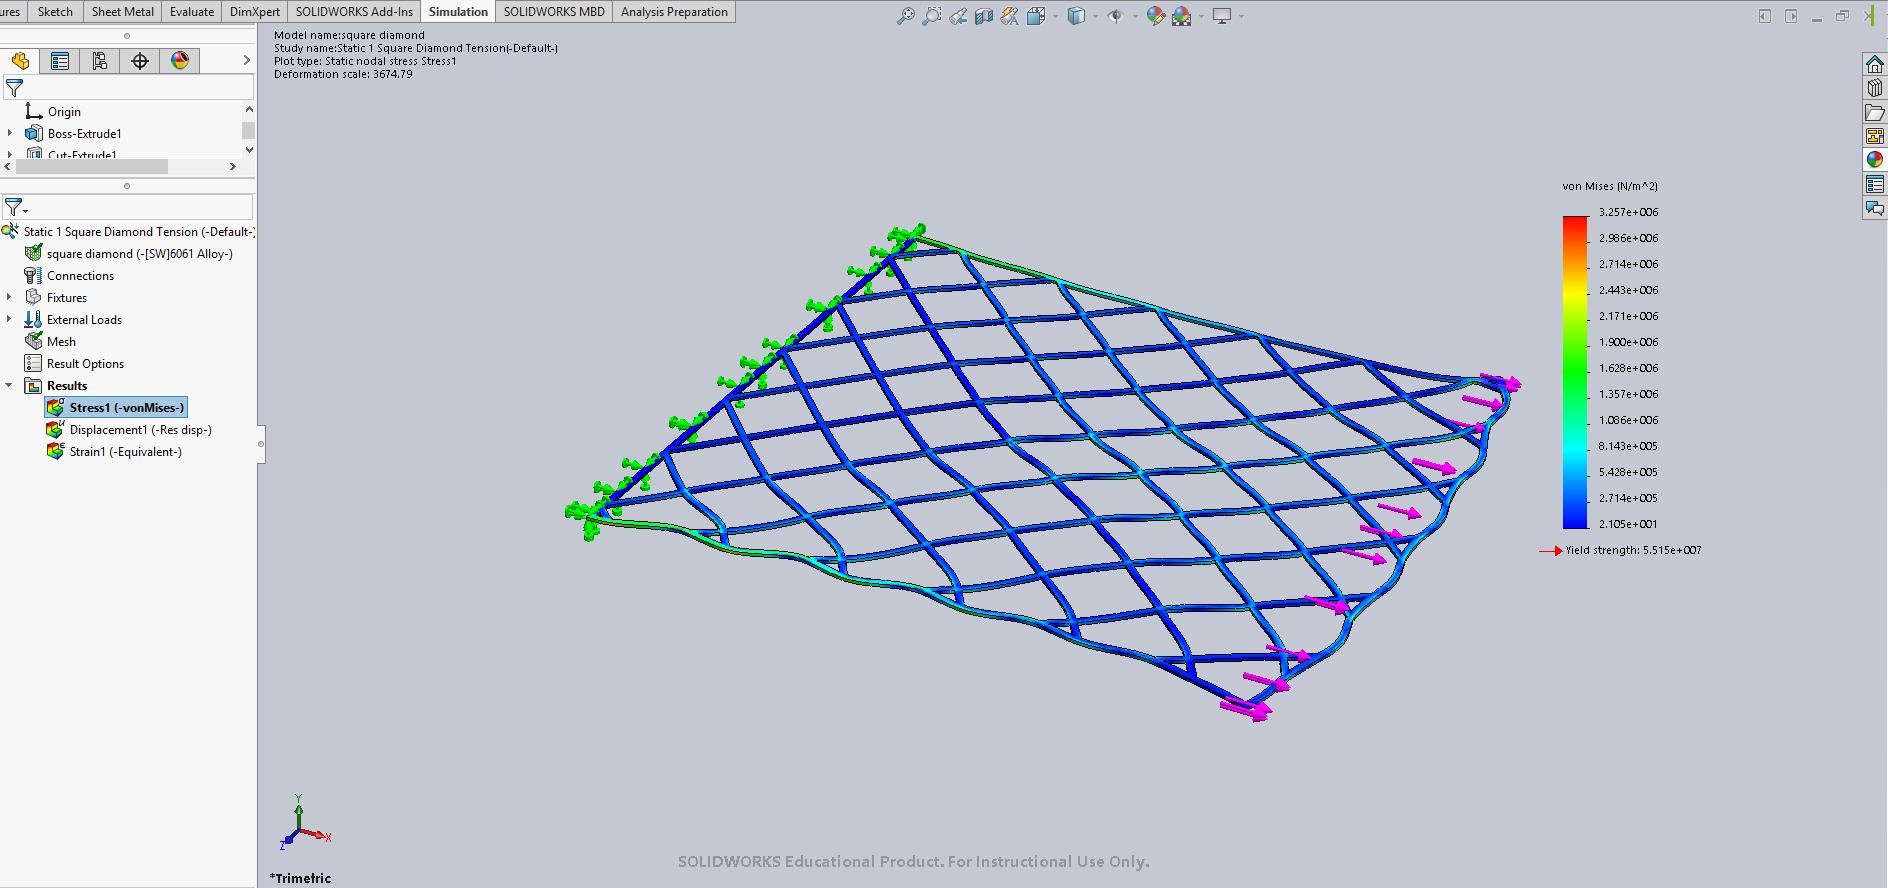
\includegraphics[width=0.8\linewidth]{./graphs/tension/square-diamond-tension-stress}

\subsubsection{Hex Tension Stress}
\label{ap:h-te-vm}
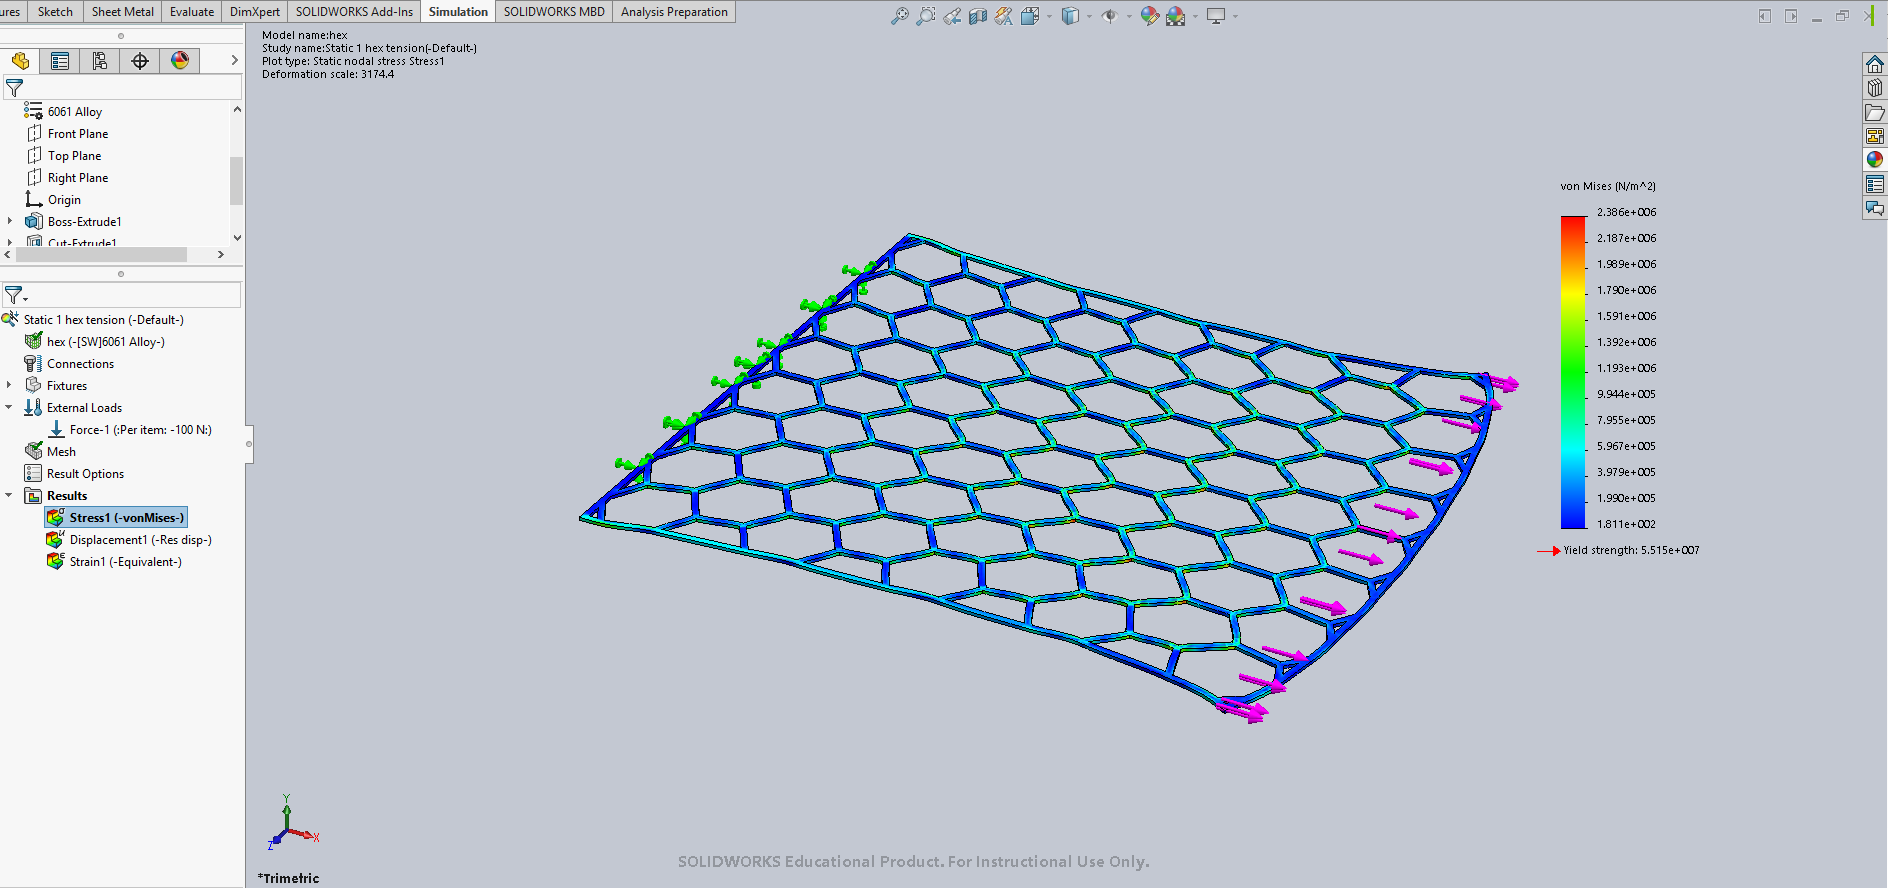
\includegraphics[width=0.8\linewidth]{./graphs/tension/hex-tension-stress}

\subsubsection{Hex Diamond Tension Stress}
\label{ap:hd-te-vm}
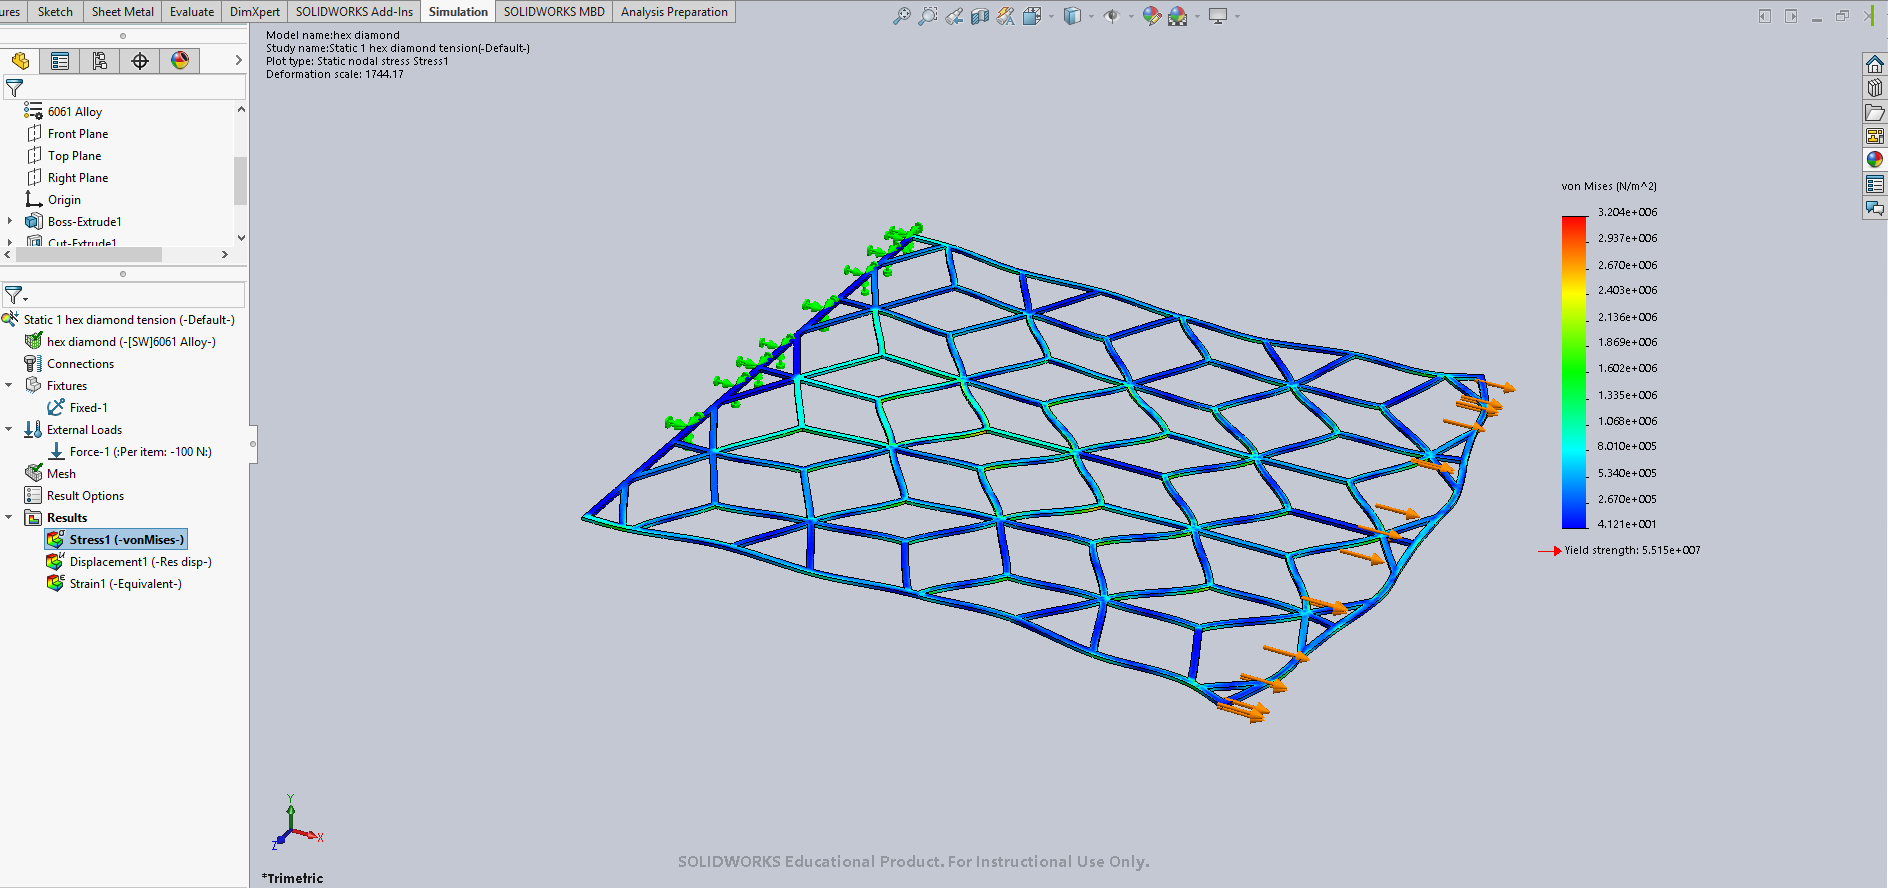
\includegraphics[width=0.8\linewidth]{./graphs/tension/hex-diamond-tension-stress}

\subsubsection{Triangle Tension Stress}
\label{ap:t-te-vm}
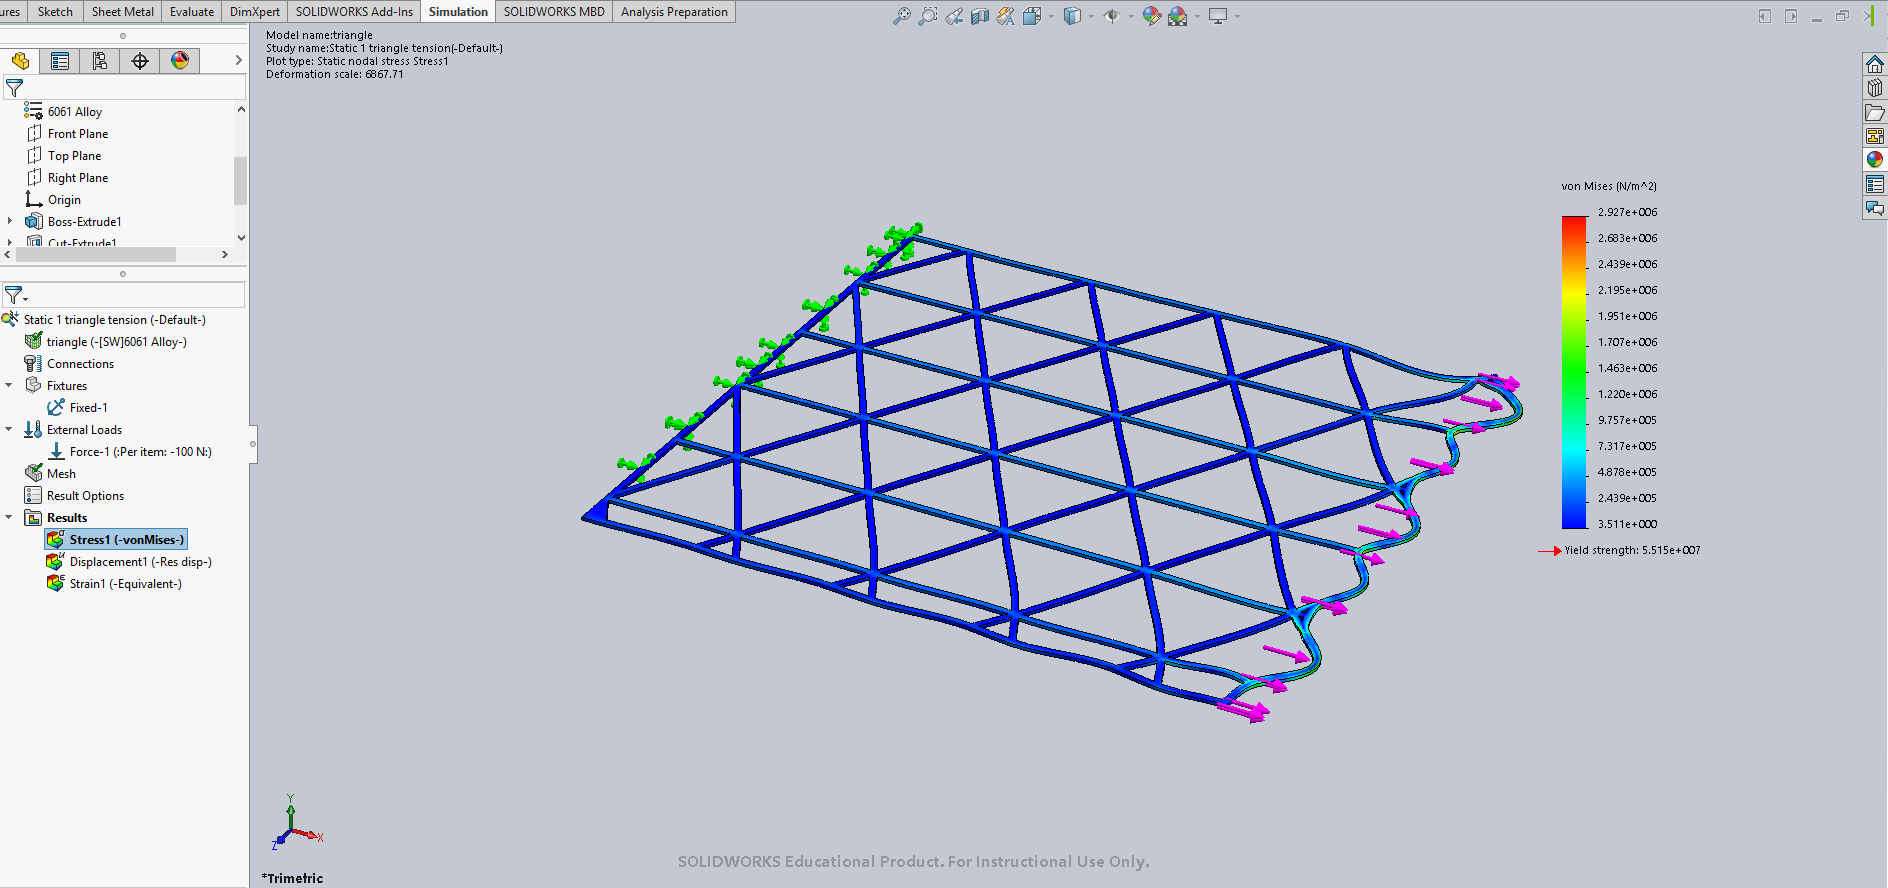
\includegraphics[width=0.8\linewidth]{./graphs/tension/triangle-tension-stress}


\subsection{Tension Strain Graphs}
\label{ap:te-es}

\subsubsection{Filled Tension Strain}
\label{ap:f-te-es}
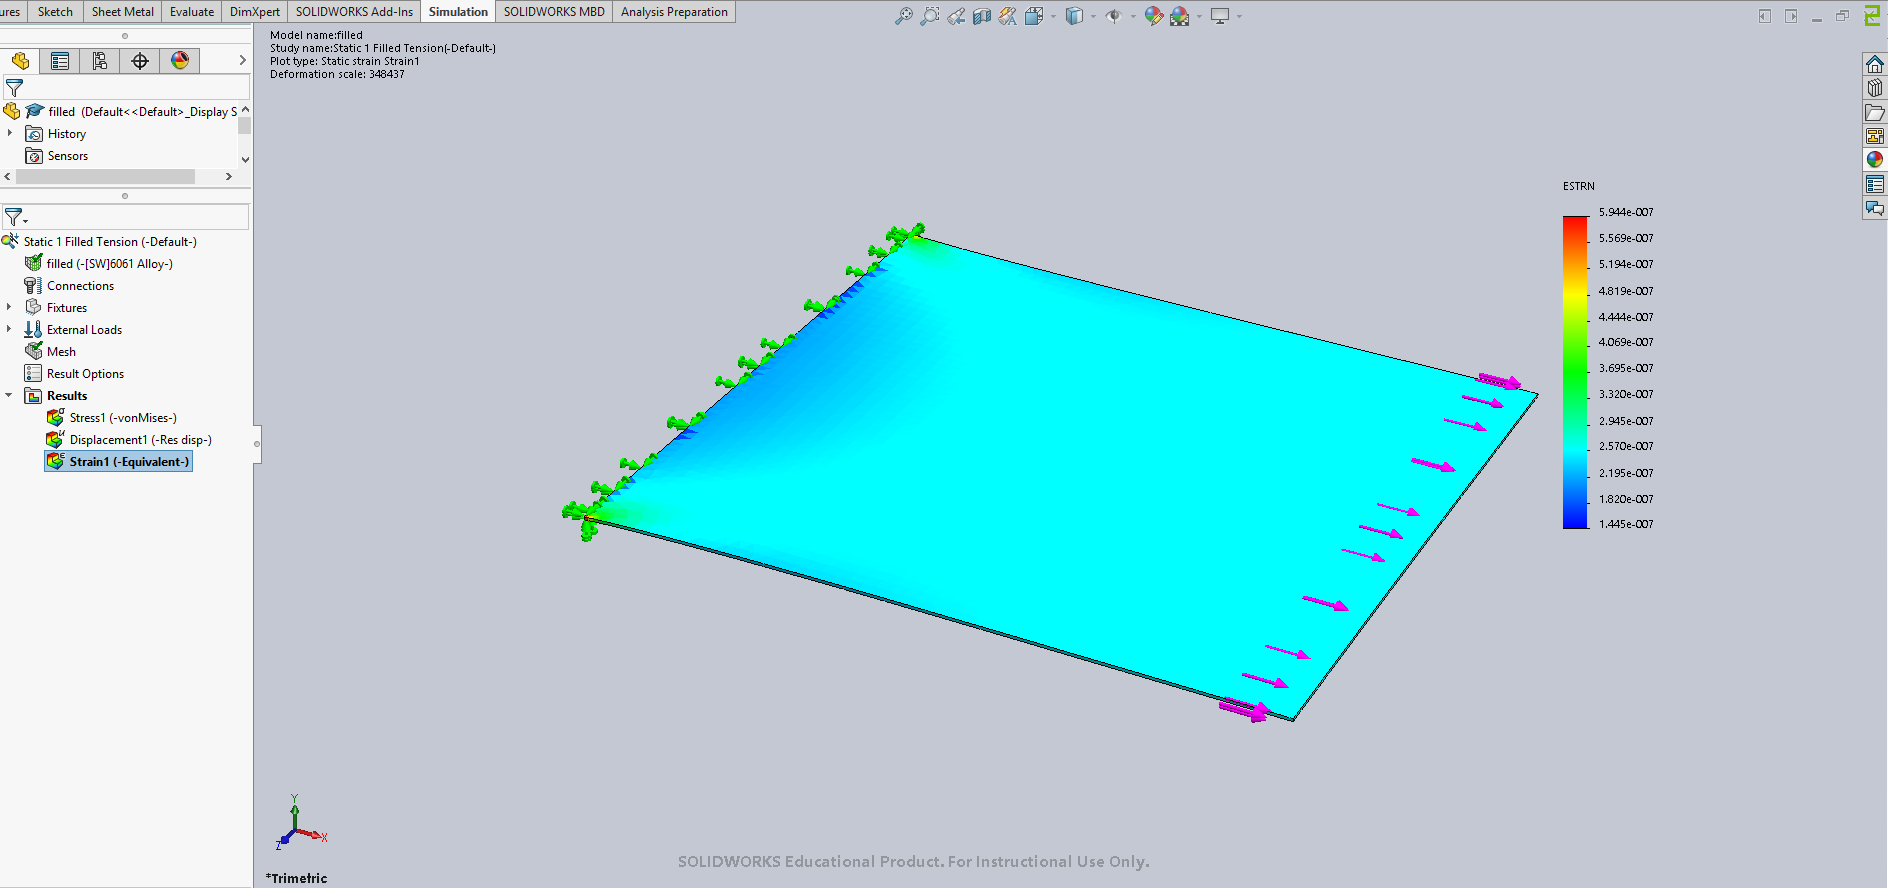
\includegraphics[width=0.8\linewidth]{./graphs/tension/filled-tension-strain}

\subsubsection{Square Tension Strain}
\label{ap:s-te-es}
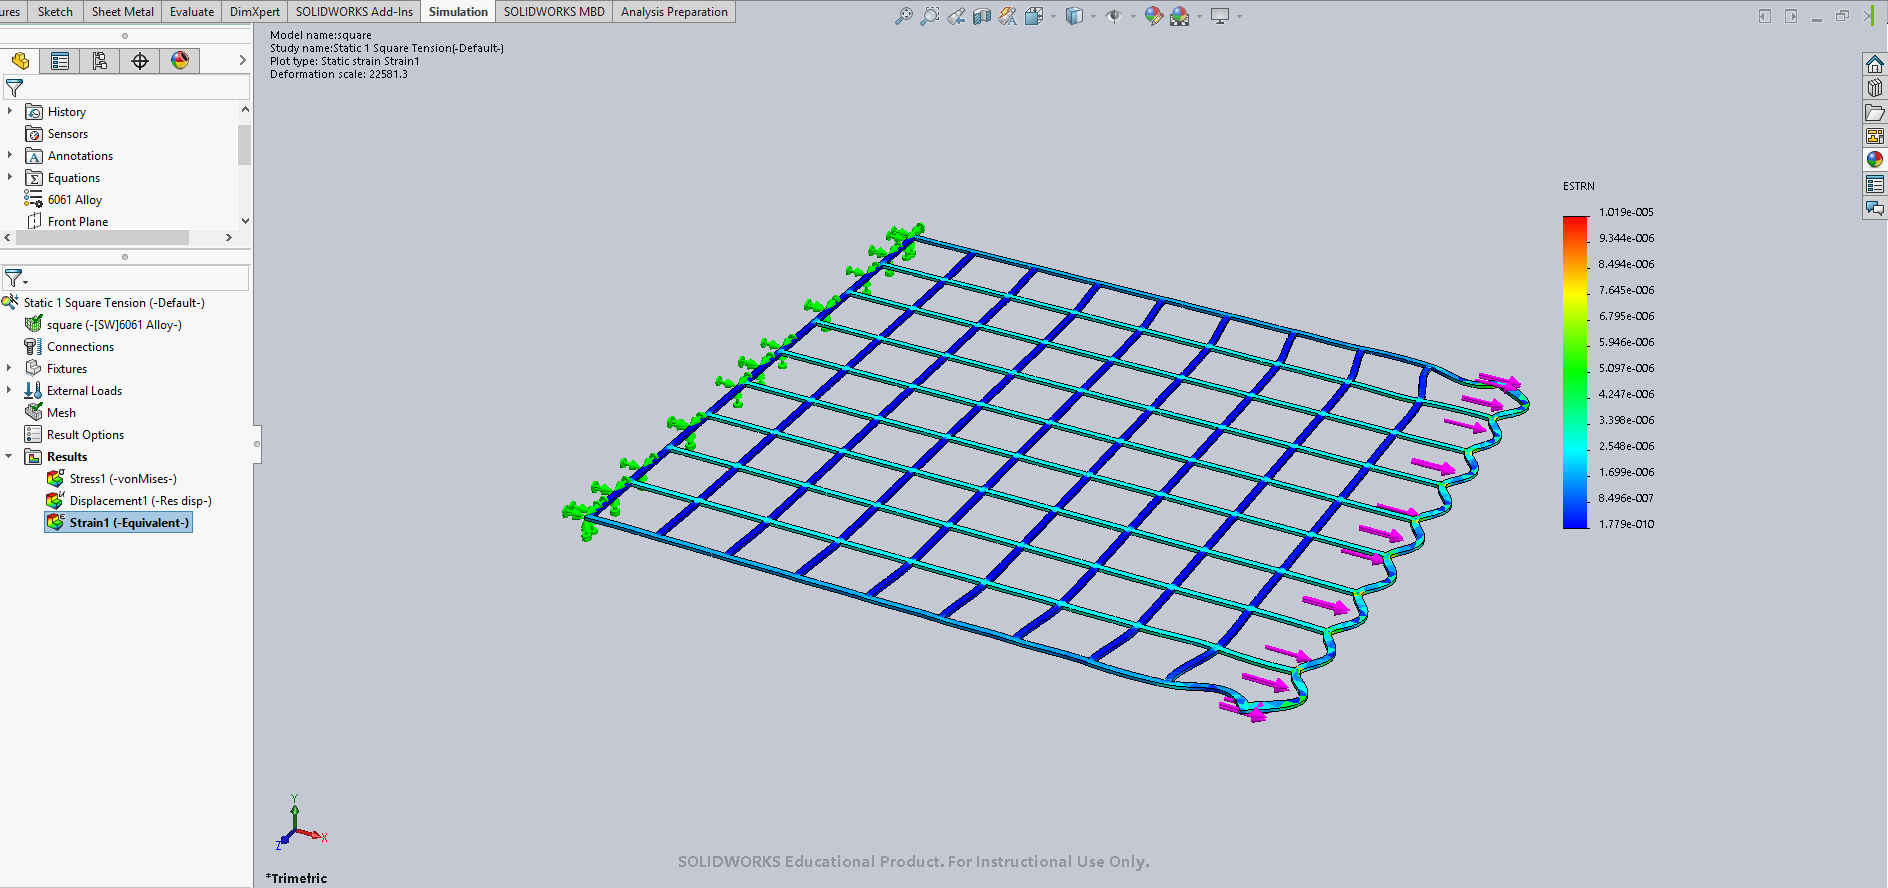
\includegraphics[width=0.8\linewidth]{./graphs/tension/square-tension-strain}

\subsubsection{Square Diamond Tension Strain}
\label{ap:sd-te-es}
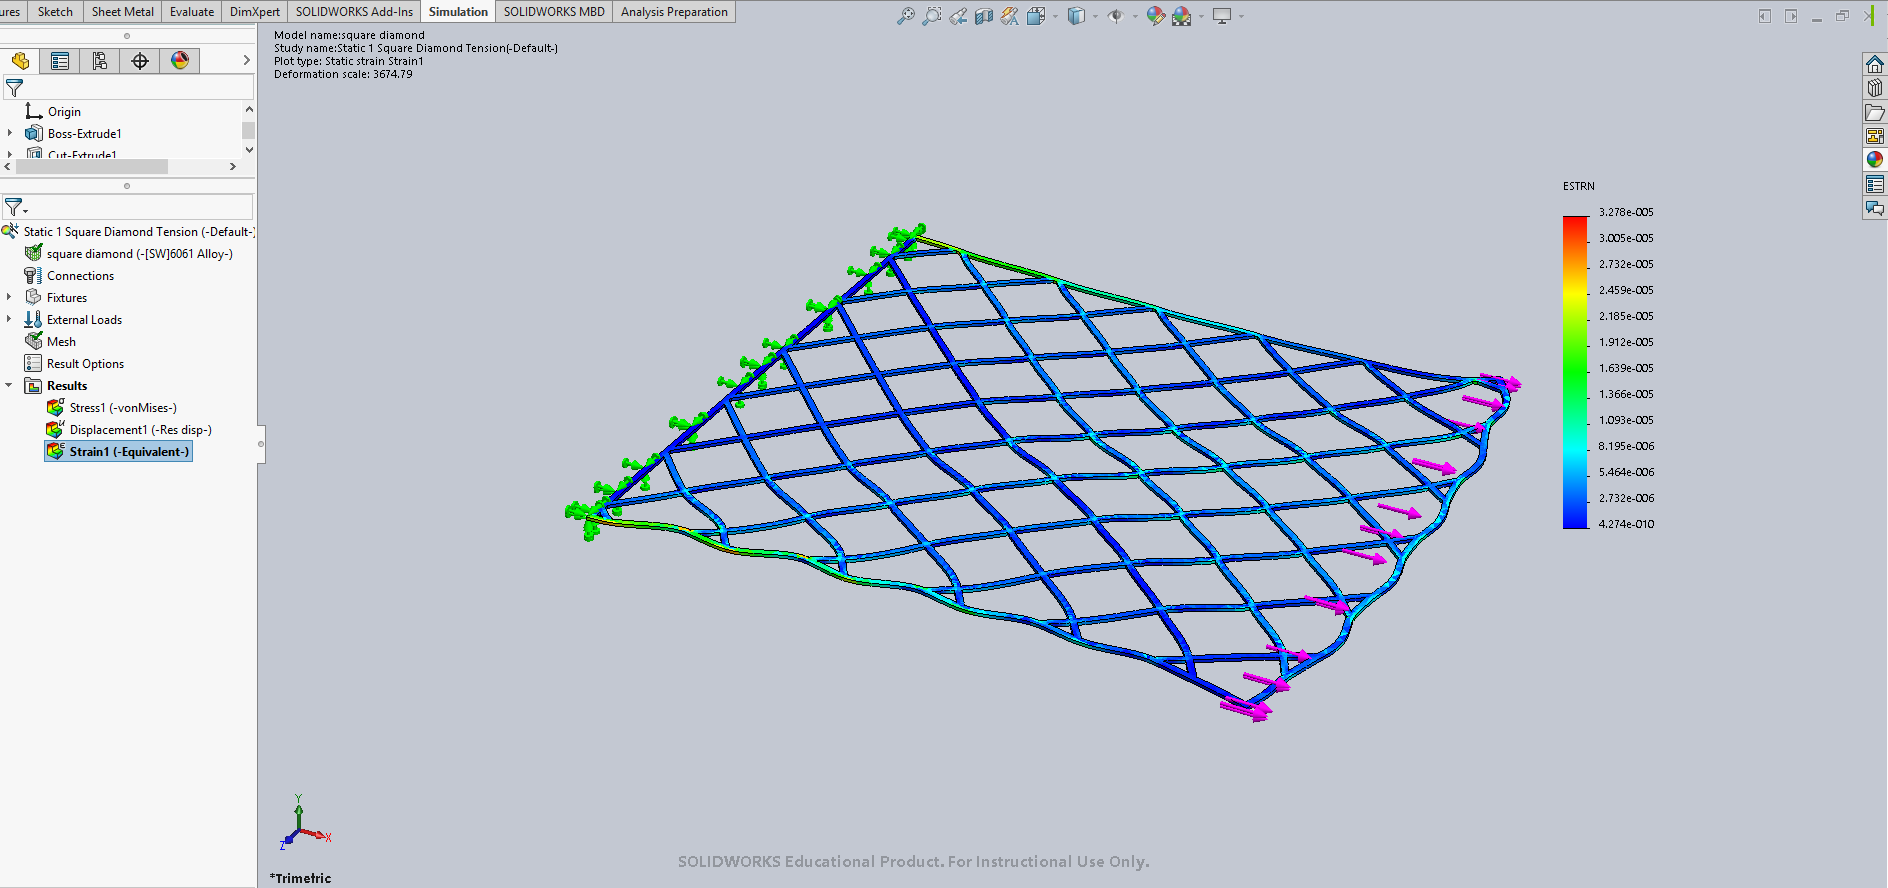
\includegraphics[width=0.8\linewidth]{./graphs/tension/square-diamond-tension-strain}

\subsubsection{Hex Tension Strain}
\label{ap:h-te-es}
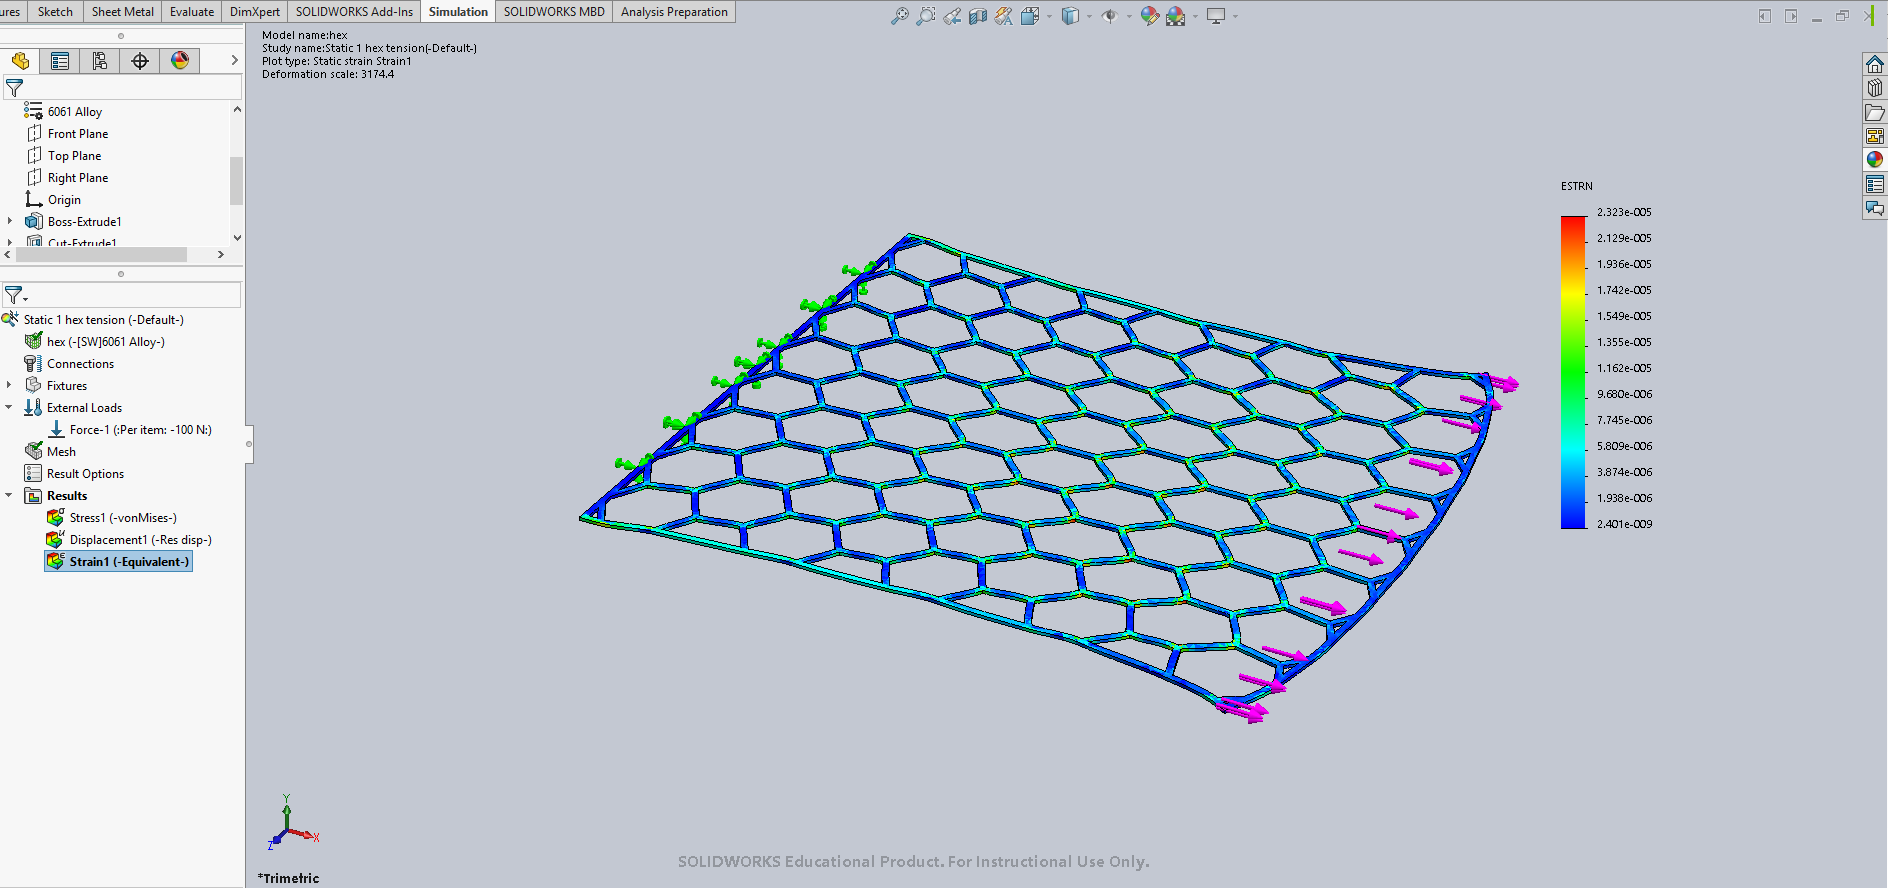
\includegraphics[width=0.8\linewidth]{./graphs/tension/hex-tension-strain}

\subsubsection{Hex Diamond Tension Strain}
\label{ap:hd-te-es}
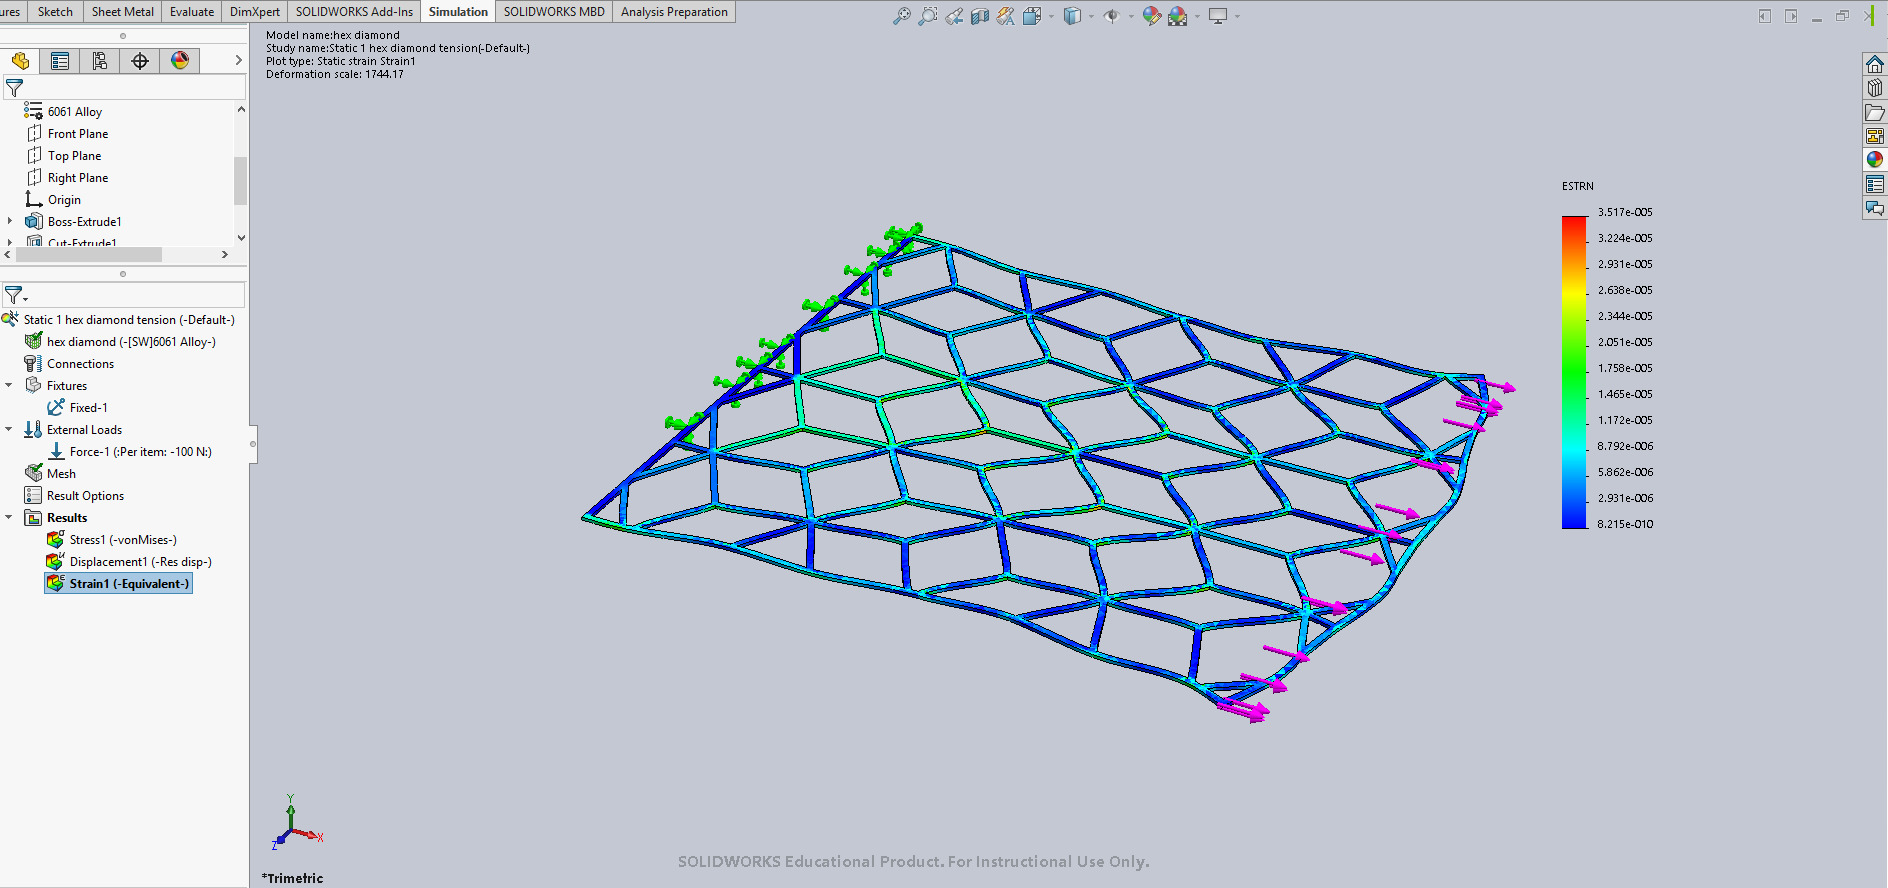
\includegraphics[width=0.8\linewidth]{./graphs/tension/hex-diamond-tension-strain}

\subsubsection{Triangle Tension Strain}
\label{ap:t-te-es}
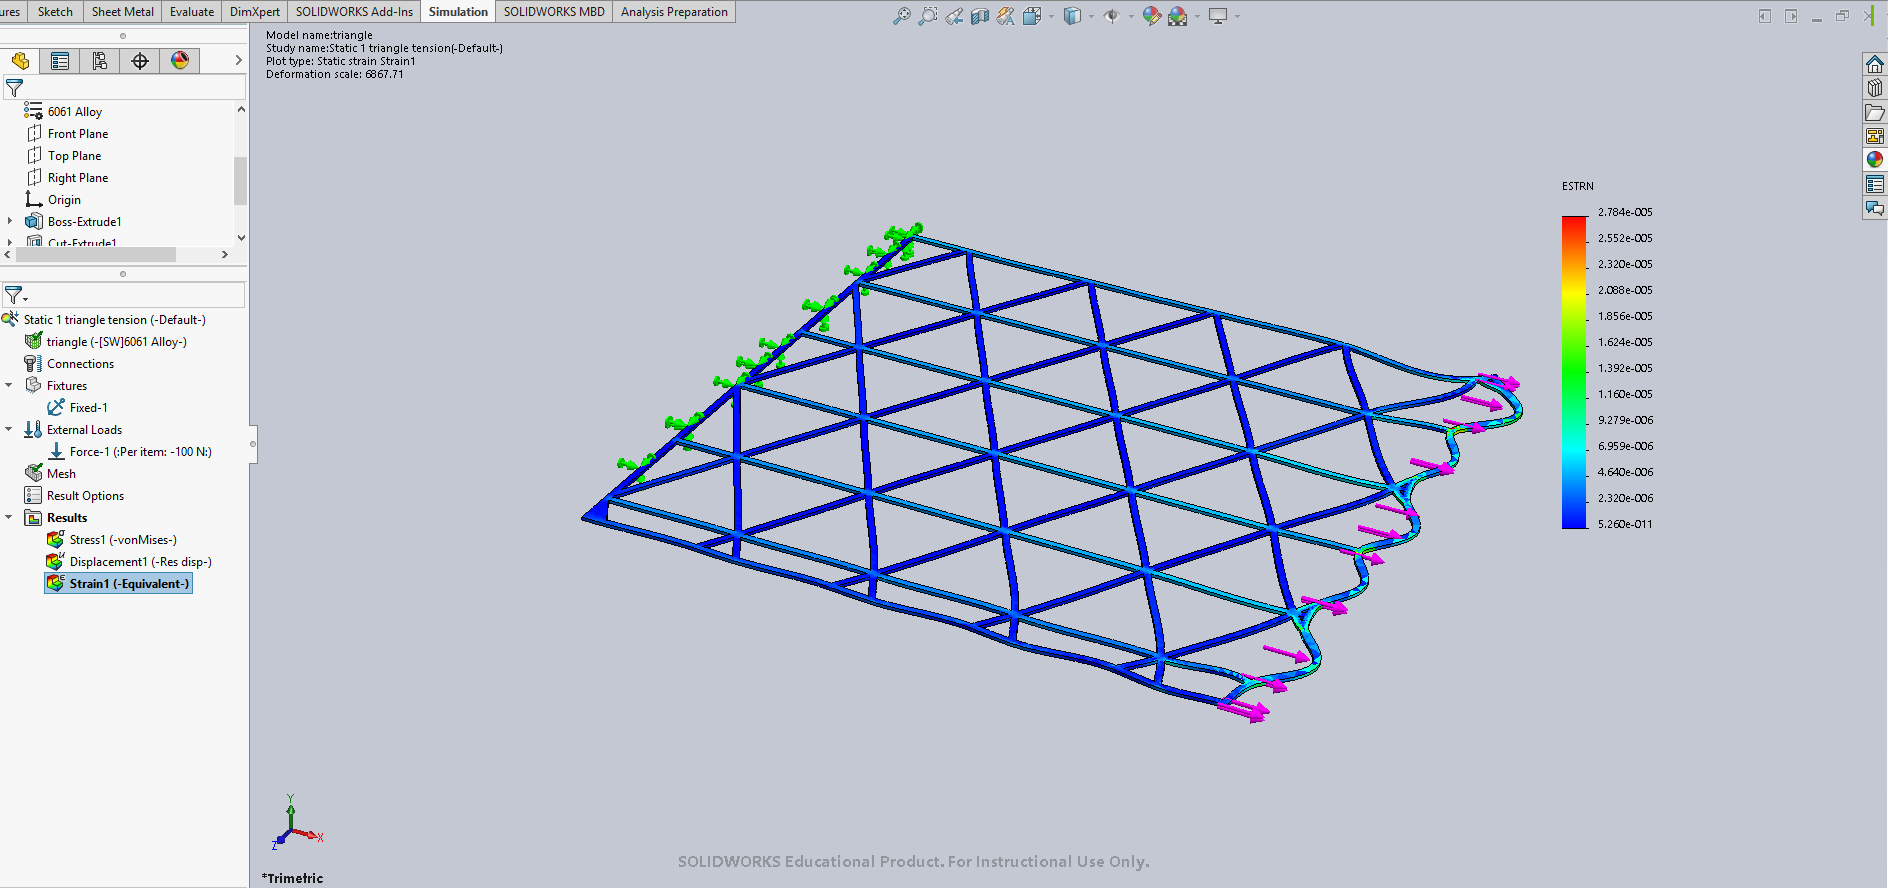
\includegraphics[width=0.8\linewidth]{./graphs/tension/triangle-tension-strain}


\subsection{Tension Displacement Graphs}
\label{ap:te-d}

\subsubsection{Filled Tension Displacement}
\label{ap:f-te-d}
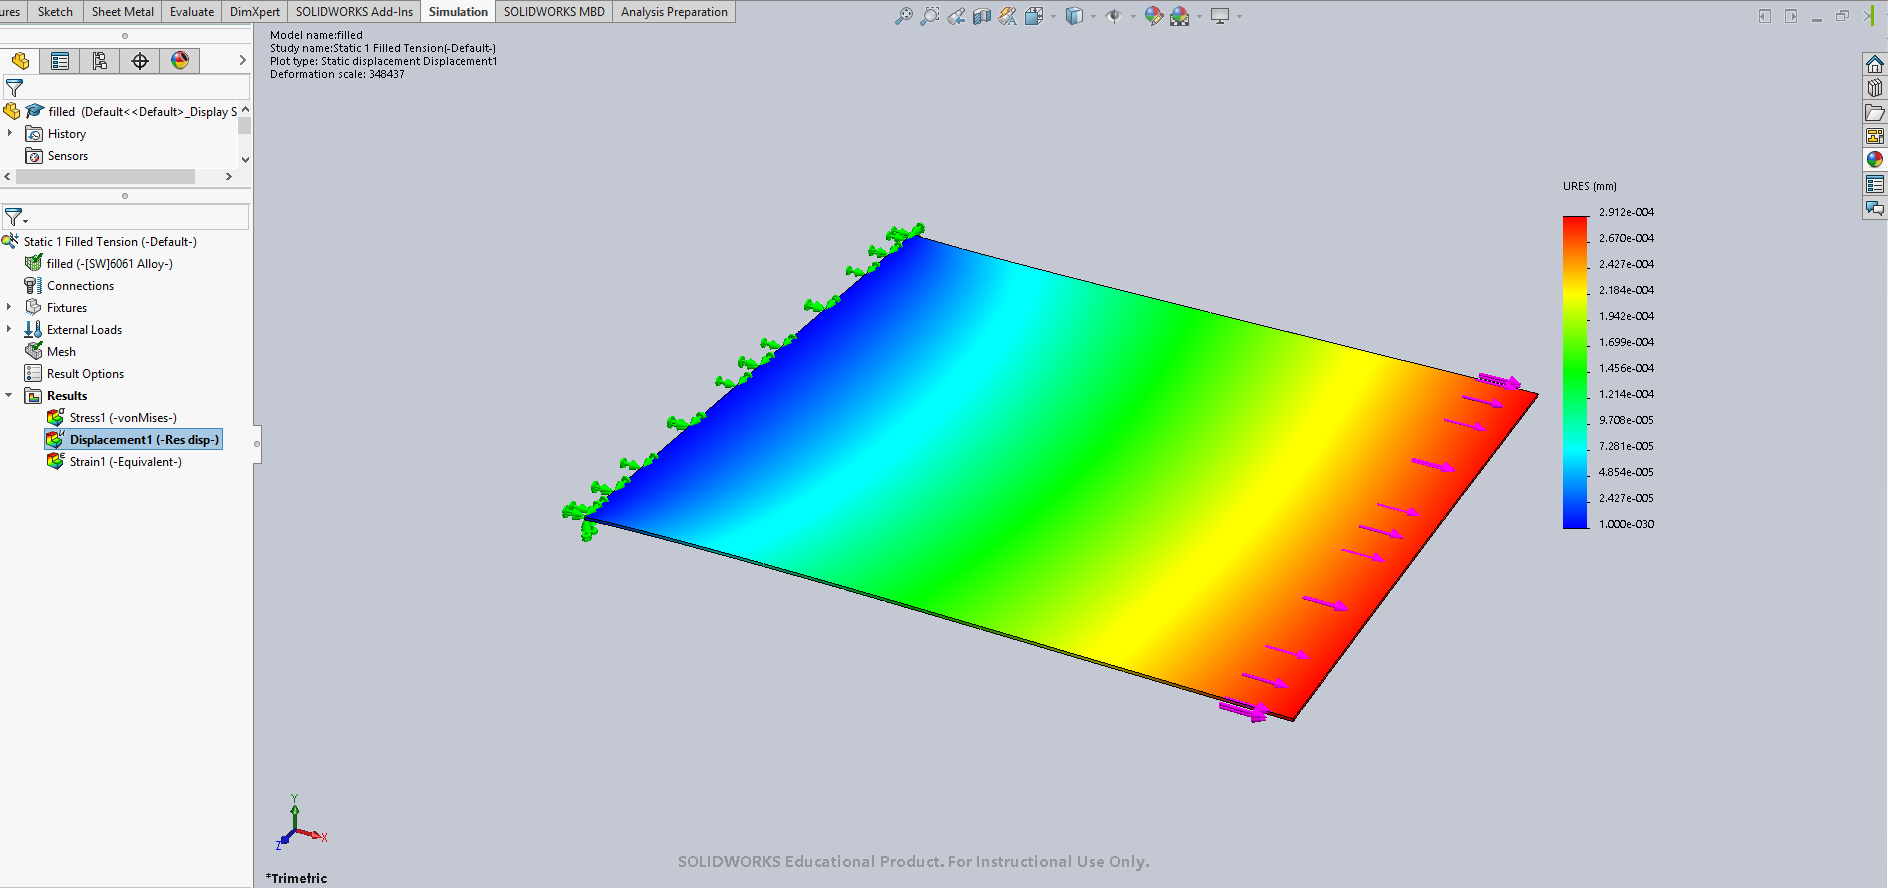
\includegraphics[width=0.8\linewidth]{./graphs/tension/filled-tension-displacement}

\subsubsection{Square Tension Displacement}
\label{ap:s-te-d}
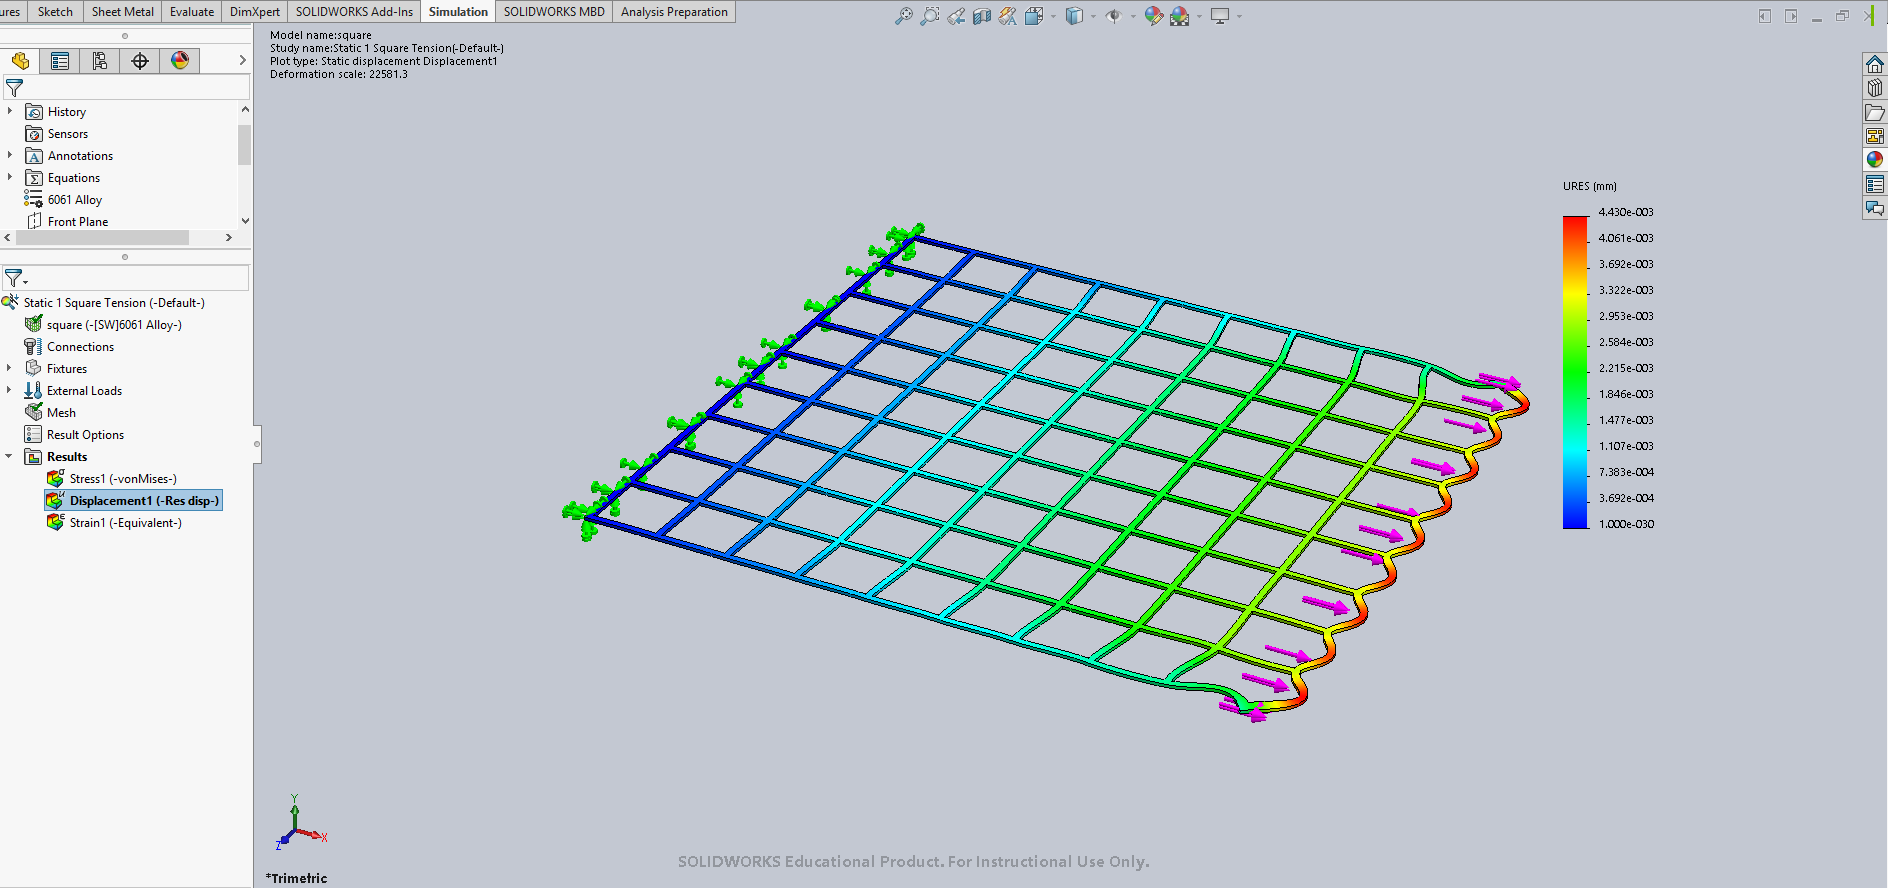
\includegraphics[width=0.8\linewidth]{./graphs/tension/square-tension-displacement}

\subsubsection{Square Diamond Tension Displacement}
\label{ap:sd-te-d}
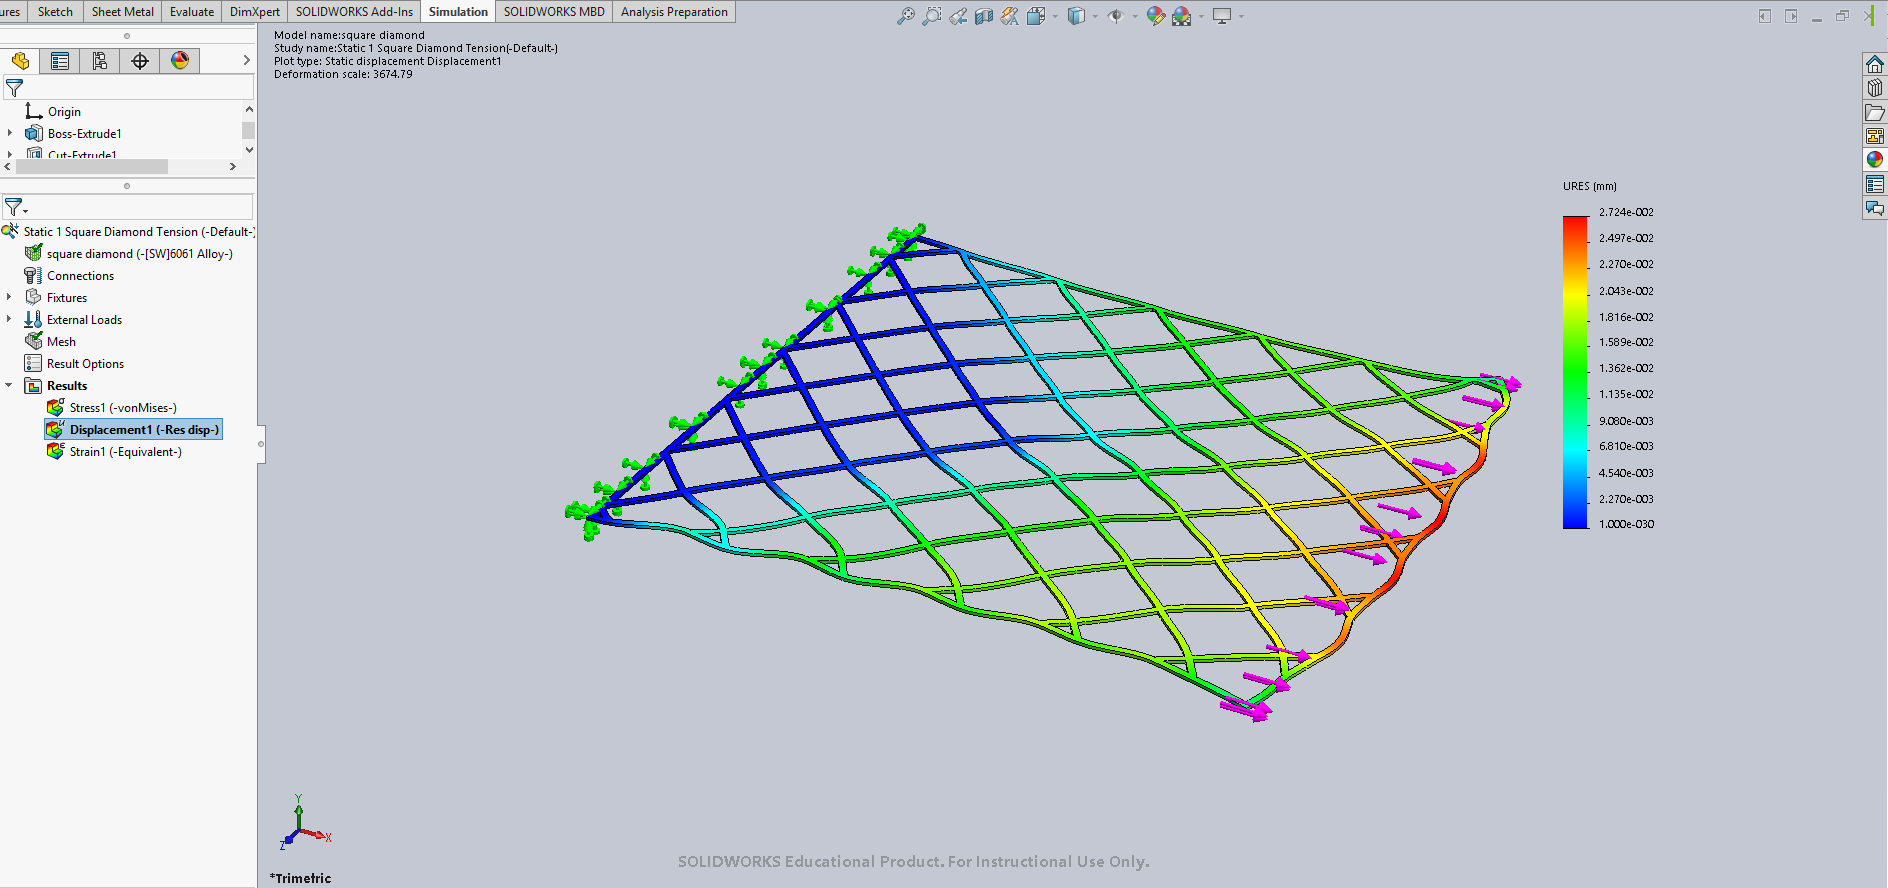
\includegraphics[width=0.8\linewidth]{./graphs/tension/square-diamond-tension-displacement}

\subsubsection{Hex Tension Displacement}
\label{ap:h-te-d}
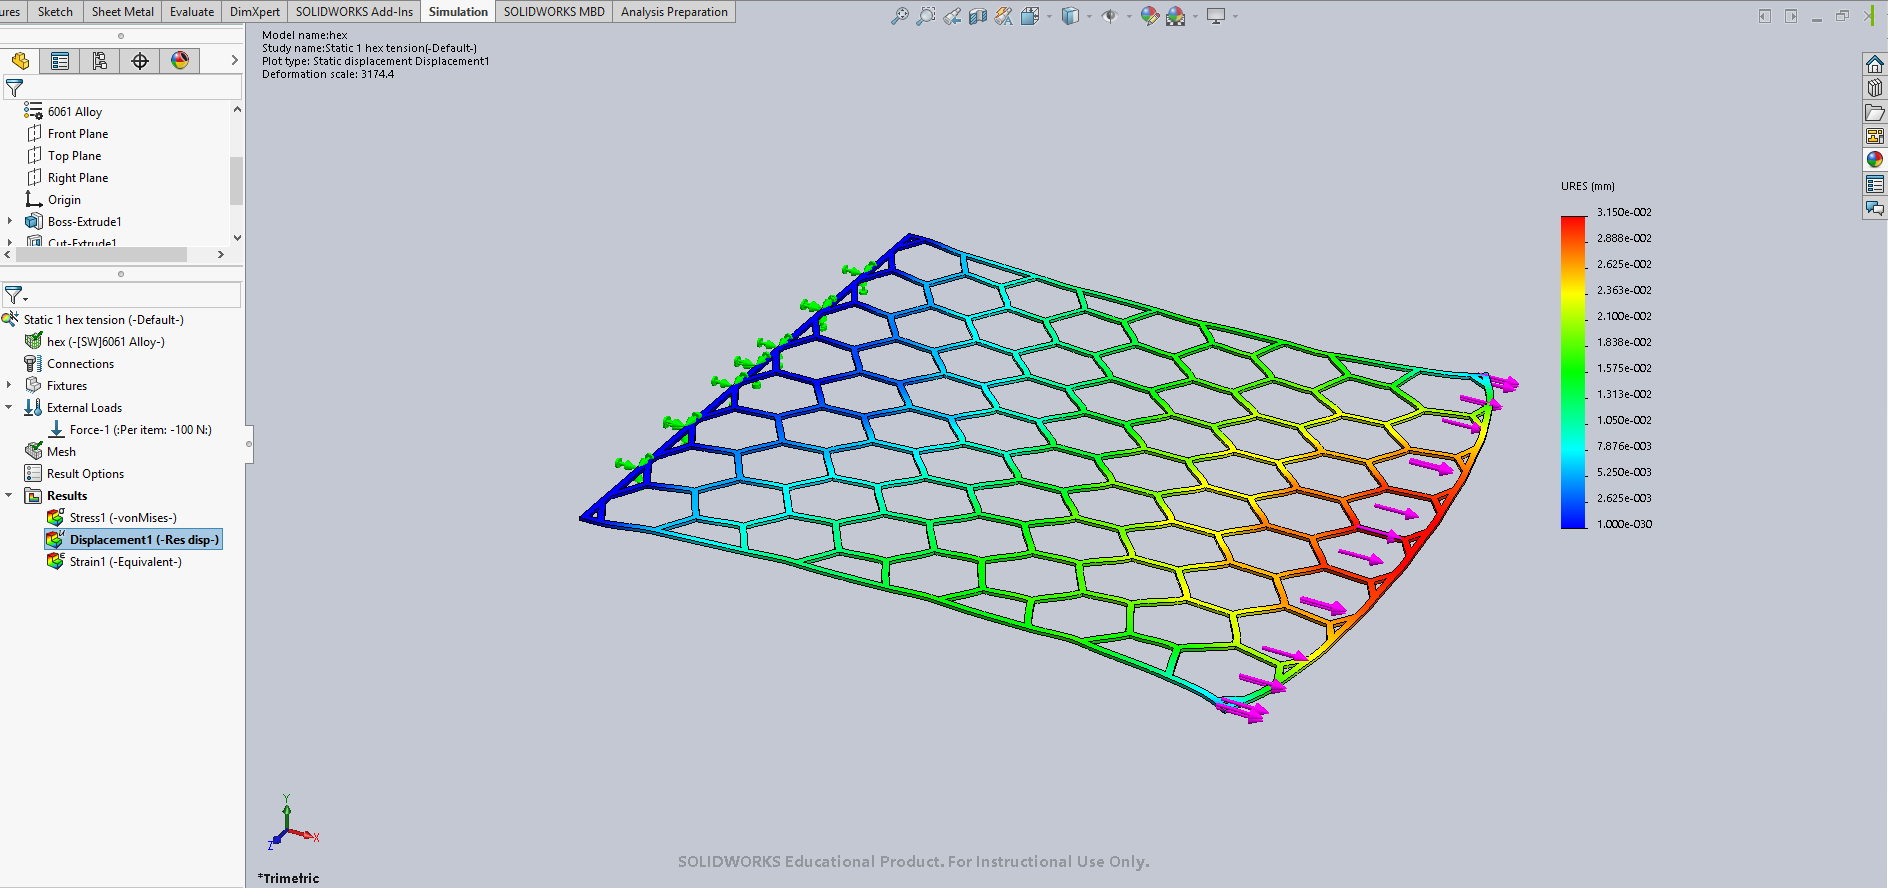
\includegraphics[width=0.8\linewidth]{./graphs/tension/hex-tension-displacement}

\subsubsection{Hex Diamond Tension Displacement}
\label{ap:hd-te-d}
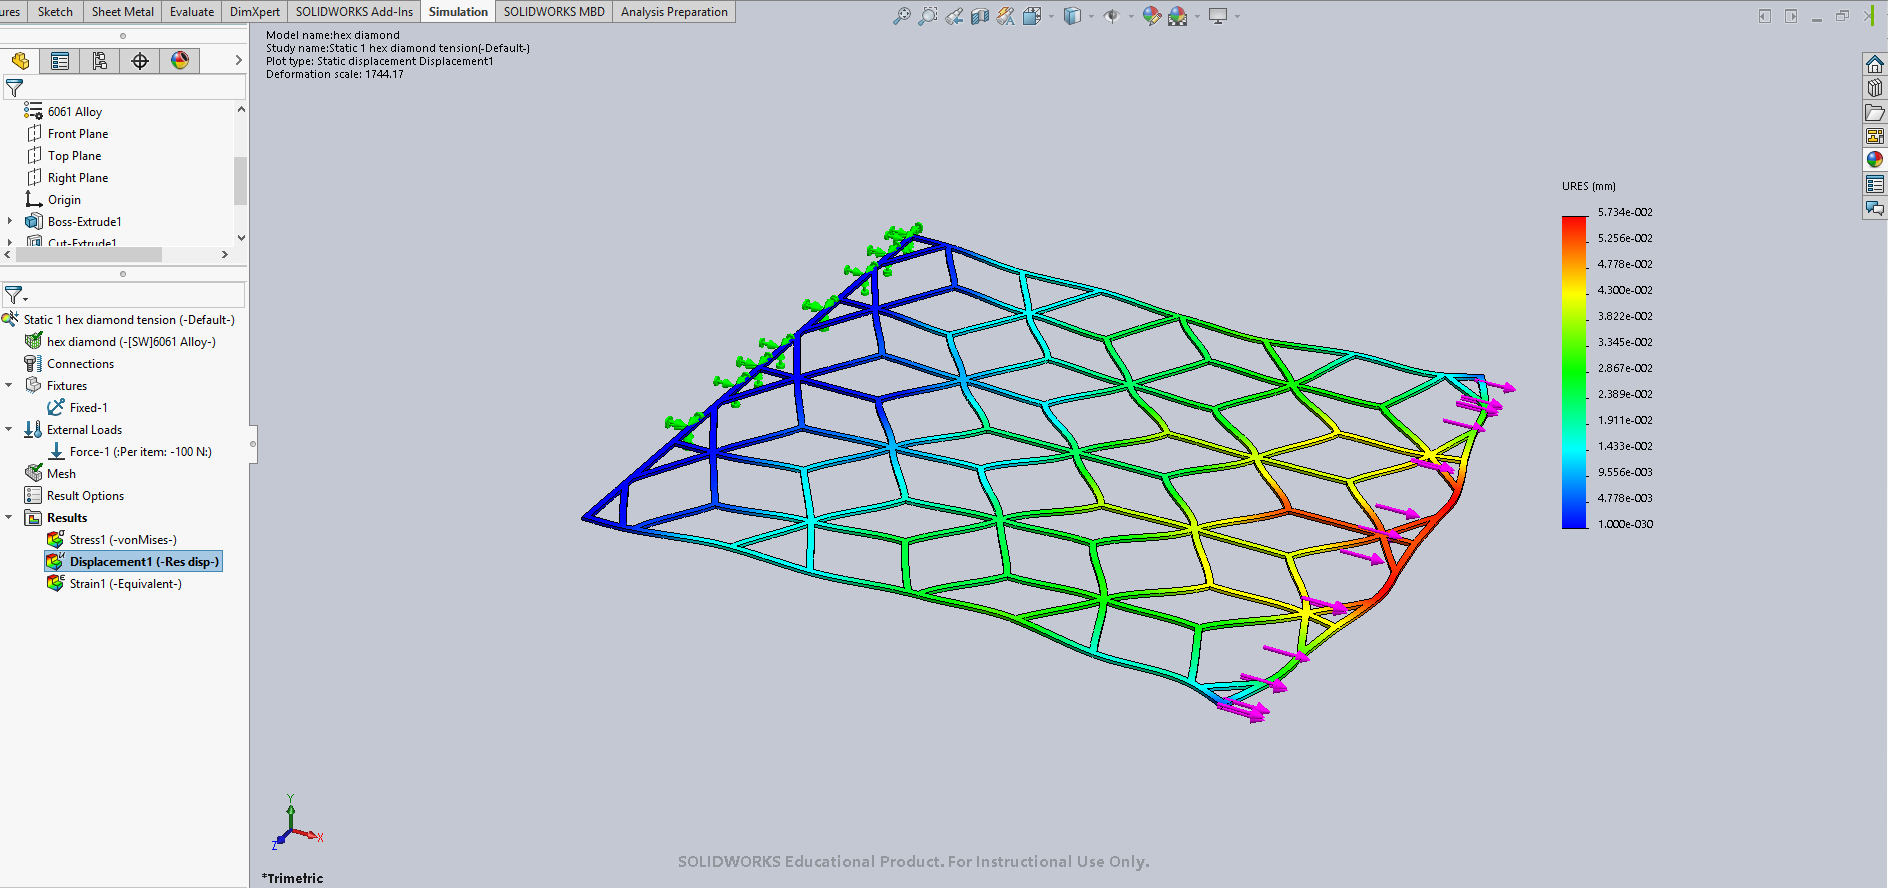
\includegraphics[width=0.8\linewidth]{./graphs/tension/hex-diamond-tension-displacement}

\subsubsection{Triangle Tension Displacement}
\label{ap:t-te-d}
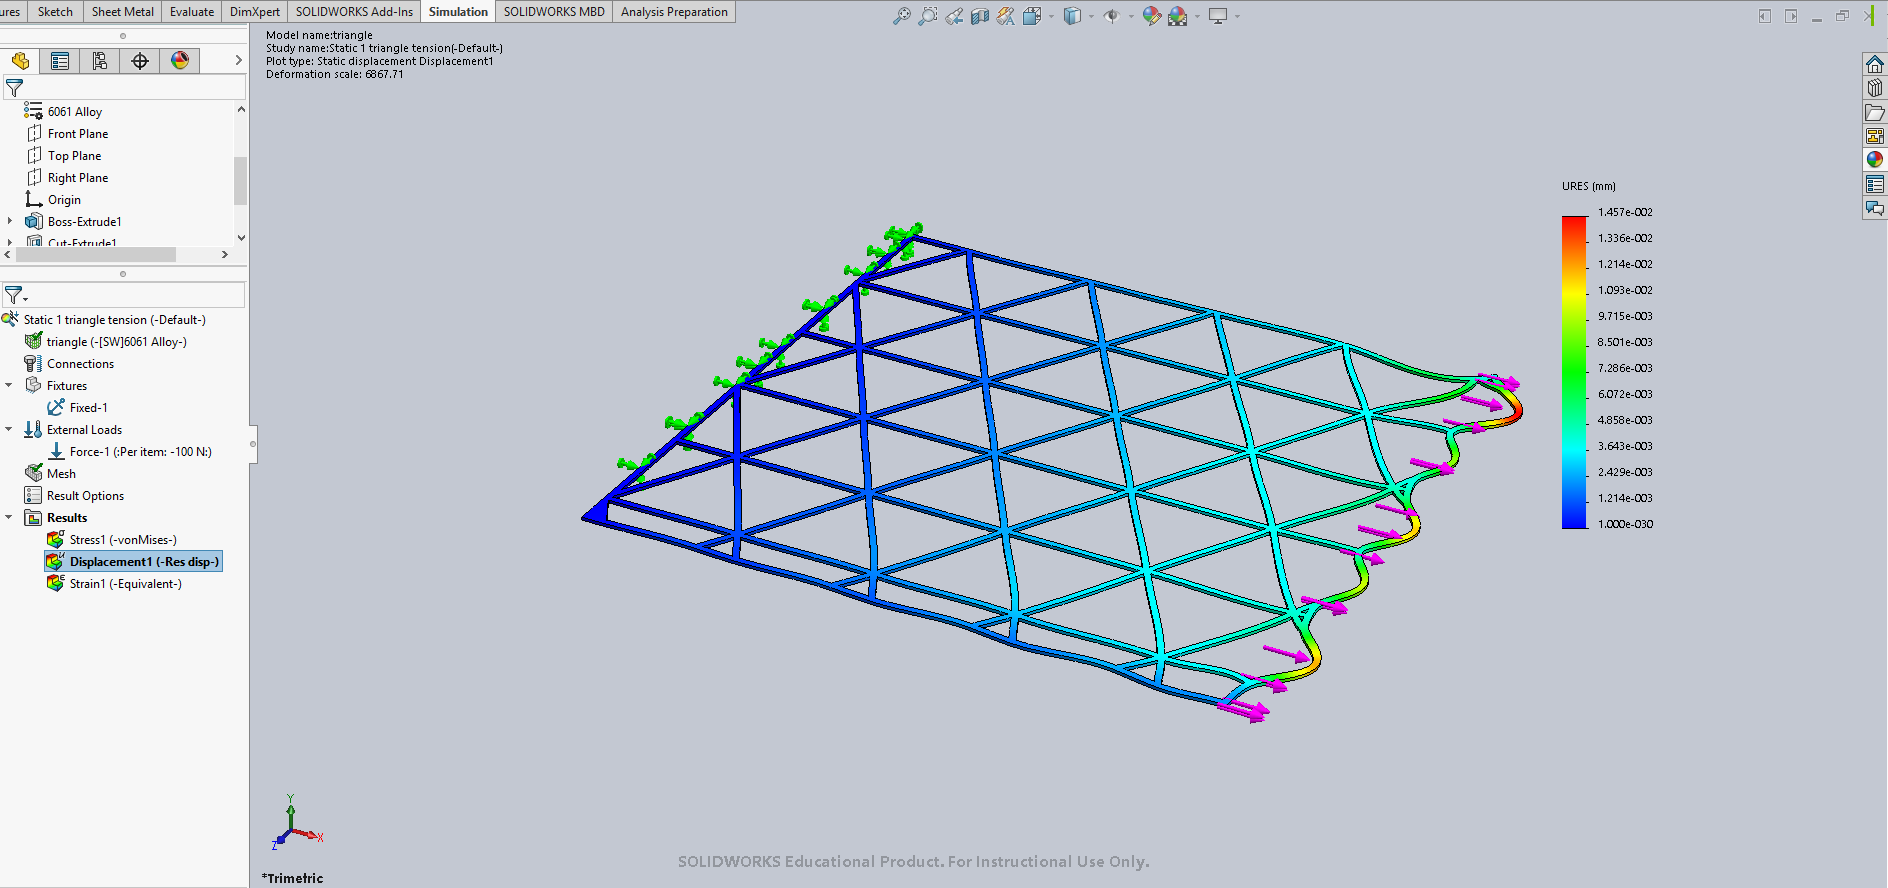
\includegraphics[width=0.8\linewidth]{./graphs/tension/triangle-tension-displacement}



\section{Compression Test Graphs}
\label{ap:c}



\subsection{Compression Stress Graphs}
\label{ap:c-vm}


\subsubsection{Filled Compression Stress}
\label{ap:f-c-vm}
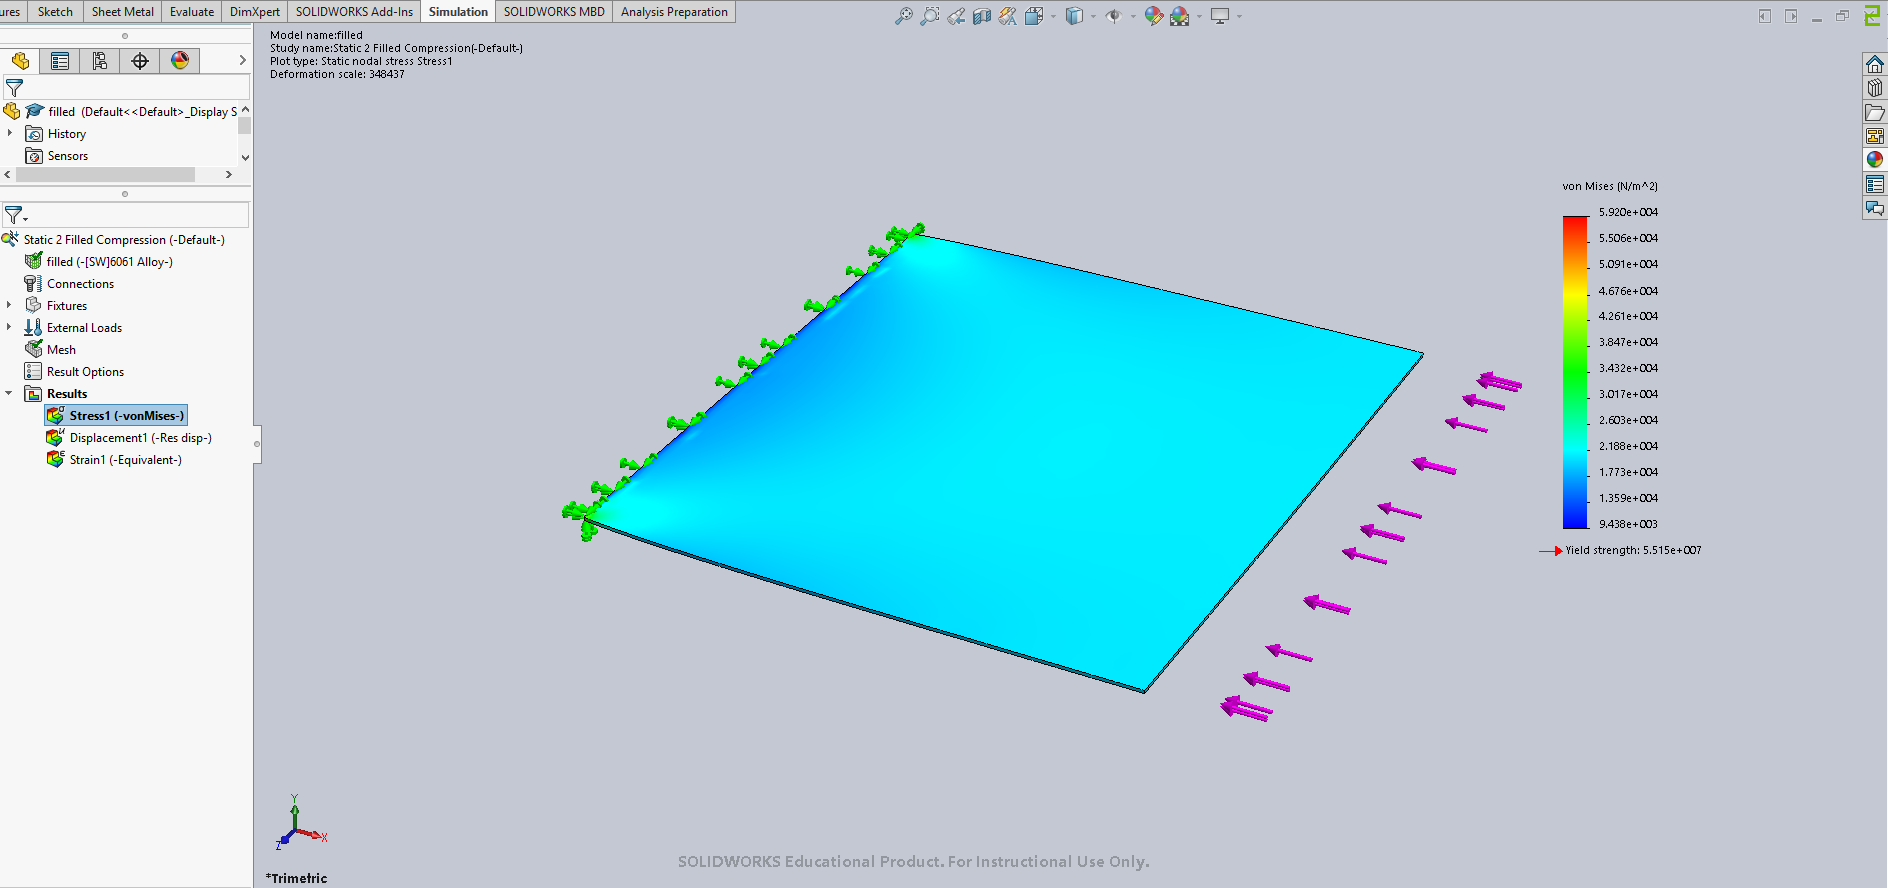
\includegraphics[width=0.8\linewidth]{./graphs/compression/filled-compression-stress}

\subsubsection{Square Compression Stress}
\label{ap:s-c-vm}
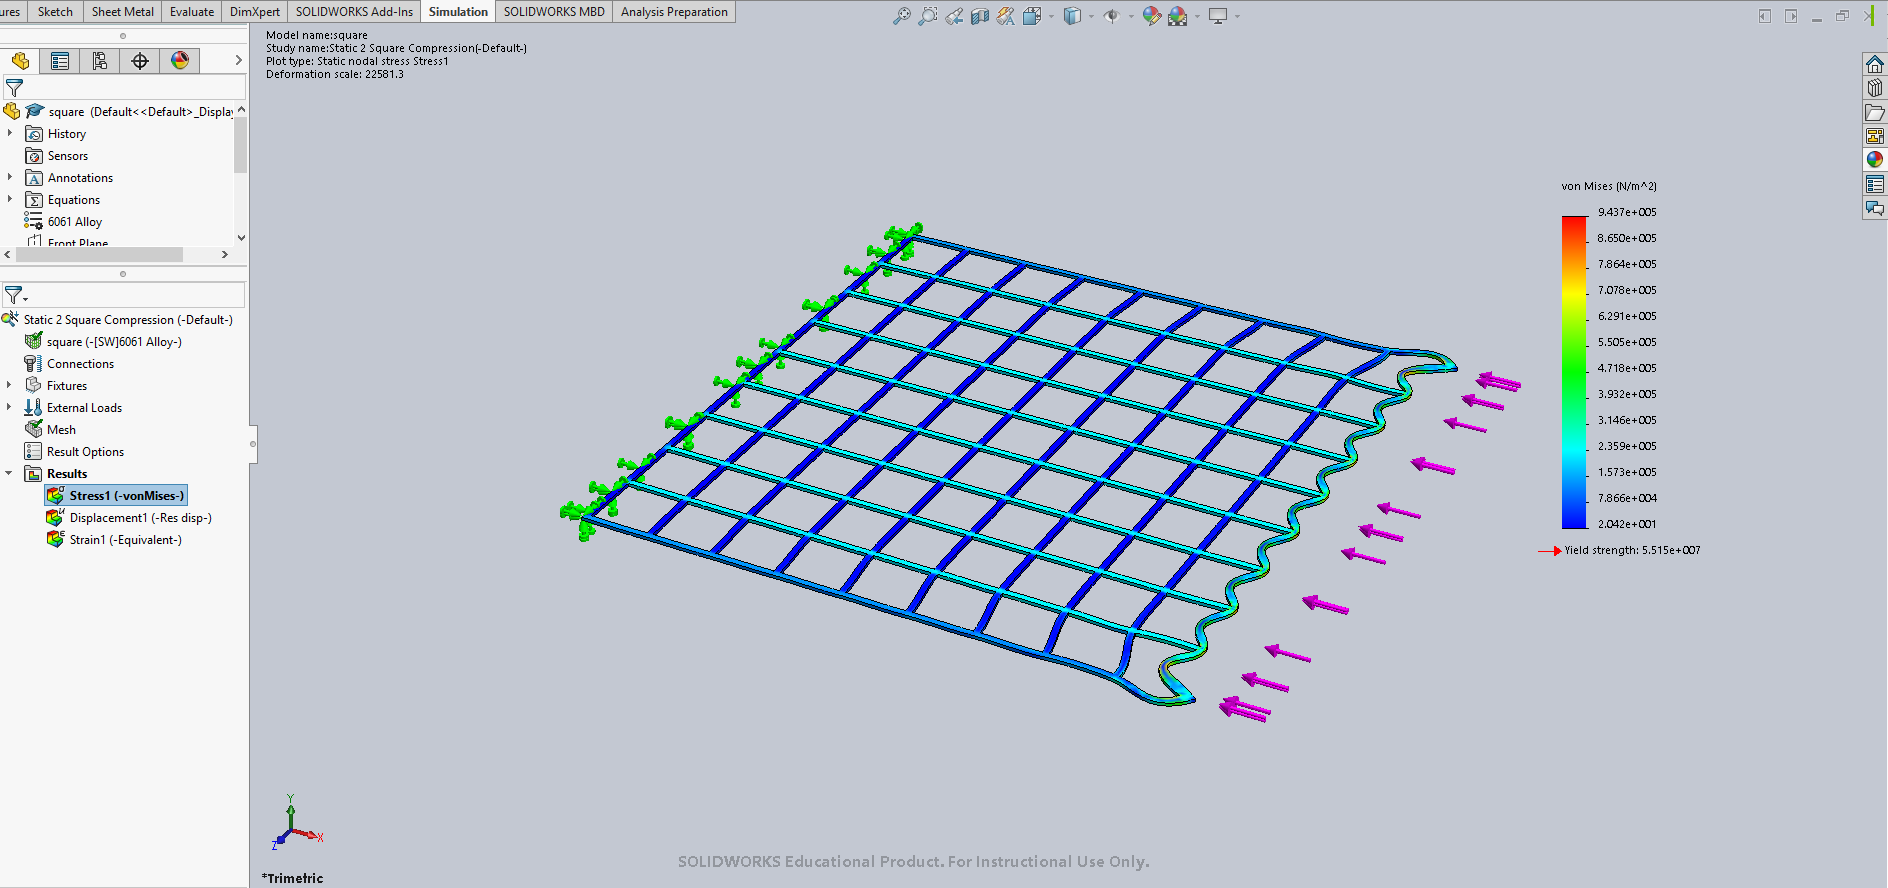
\includegraphics[width=0.8\linewidth]{./graphs/compression/square-compression-stress}

\subsubsection{Square Diamond Compression Stress}
\label{ap:sd-c-vm}
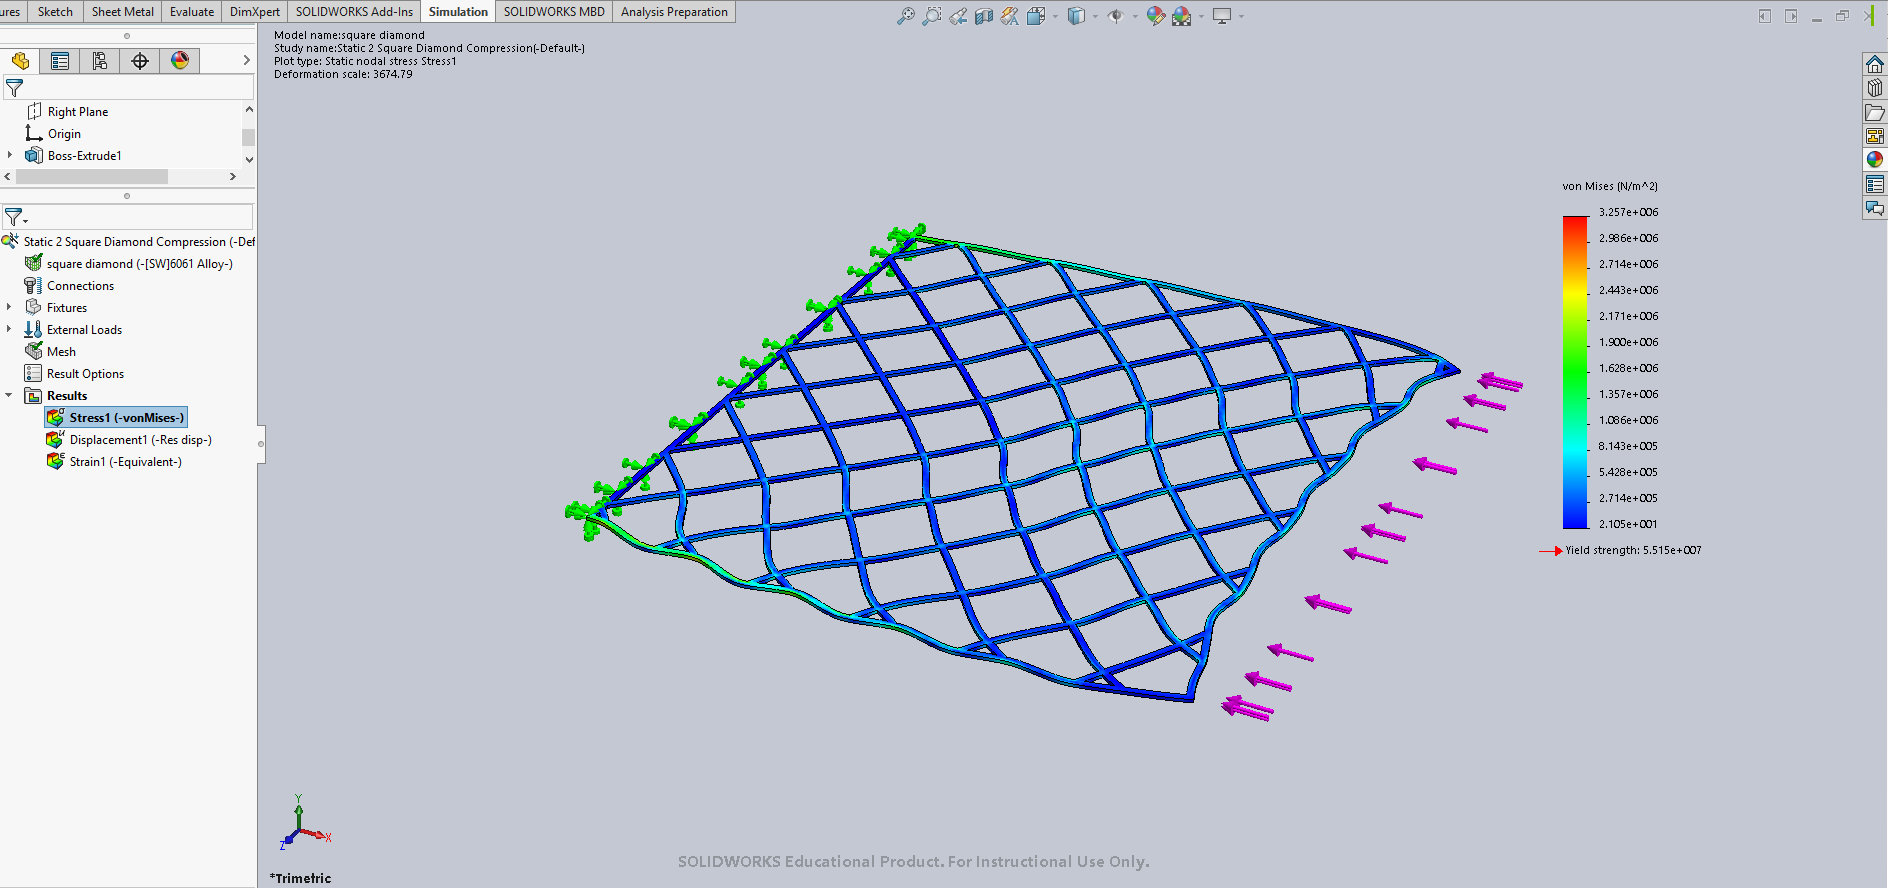
\includegraphics[width=0.8\linewidth]{./graphs/compression/square-diamond-compression-stress}

\subsubsection{Hex Compression Stress}
\label{ap:h-c-vm}
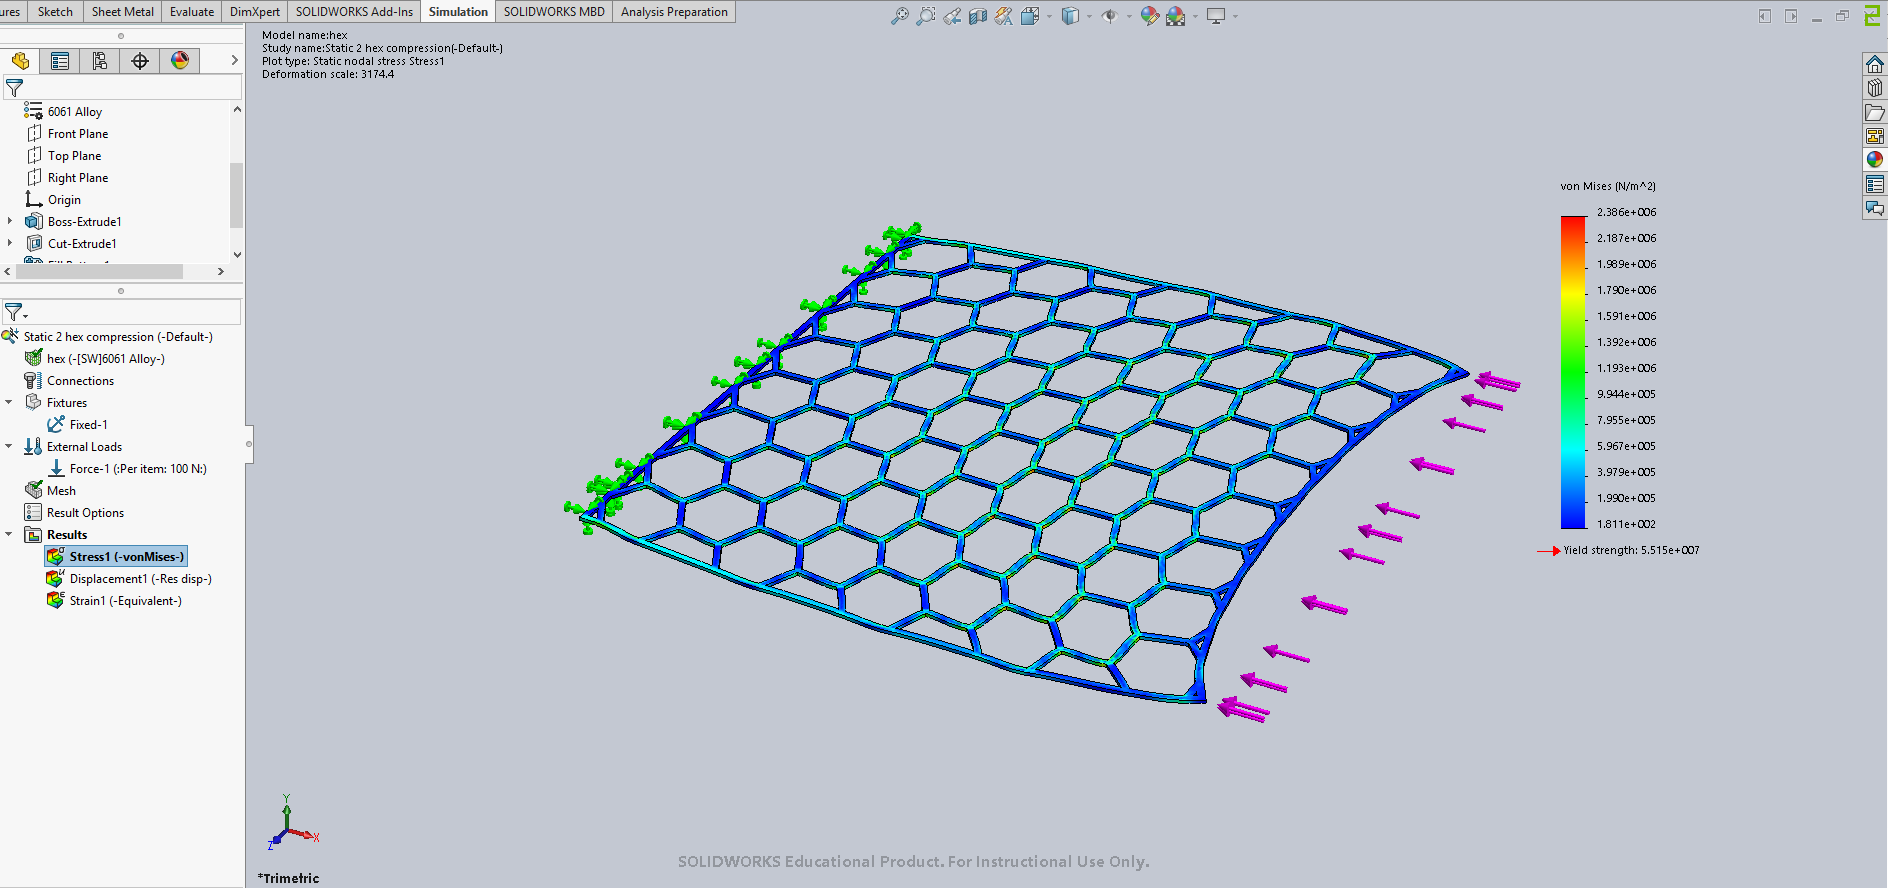
\includegraphics[width=0.8\linewidth]{./graphs/compression/hex-compression-stress}

\subsubsection{Hex Diamond Compression Stress}
\label{ap:hd-c-vm}
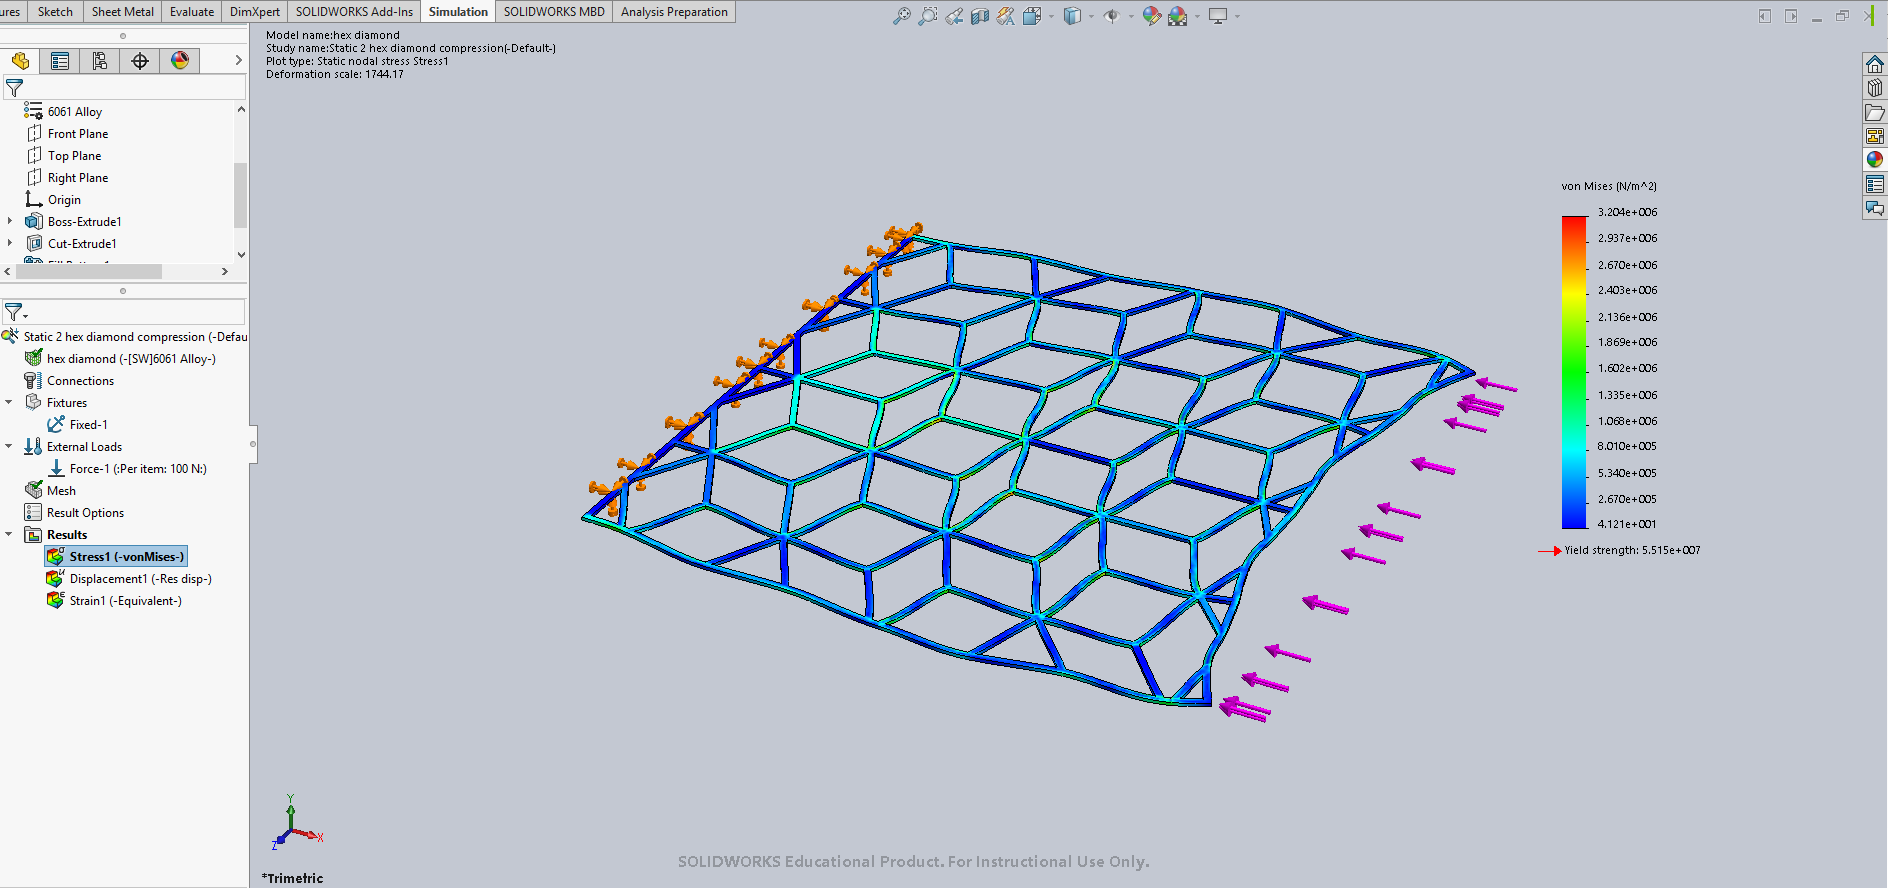
\includegraphics[width=0.8\linewidth]{./graphs/compression/hex-diamond-compression-stress}

\subsubsection{Triangle Compression Stress}
\label{ap:t-c-vm}
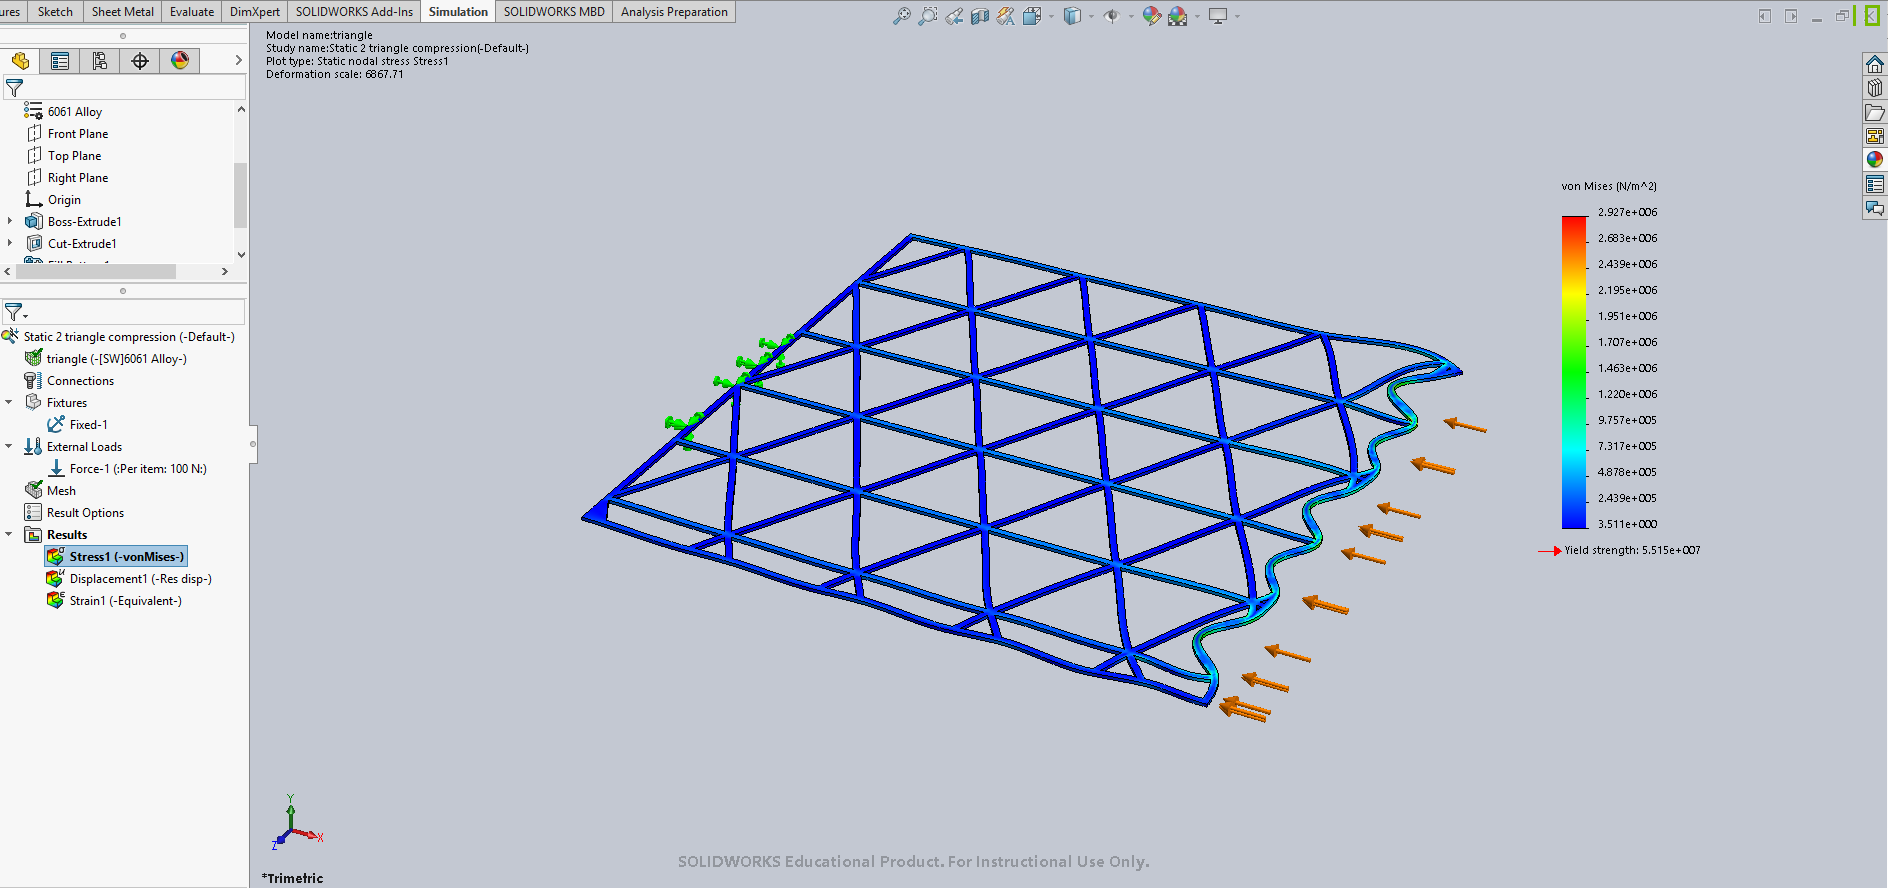
\includegraphics[width=0.8\linewidth]{./graphs/compression/triangle-compression-stress}


\subsection{Compression Strain Graphs}
\label{ap:c-es}

\subsubsection{Filled Compression Strain}
\label{ap:f-c-es}
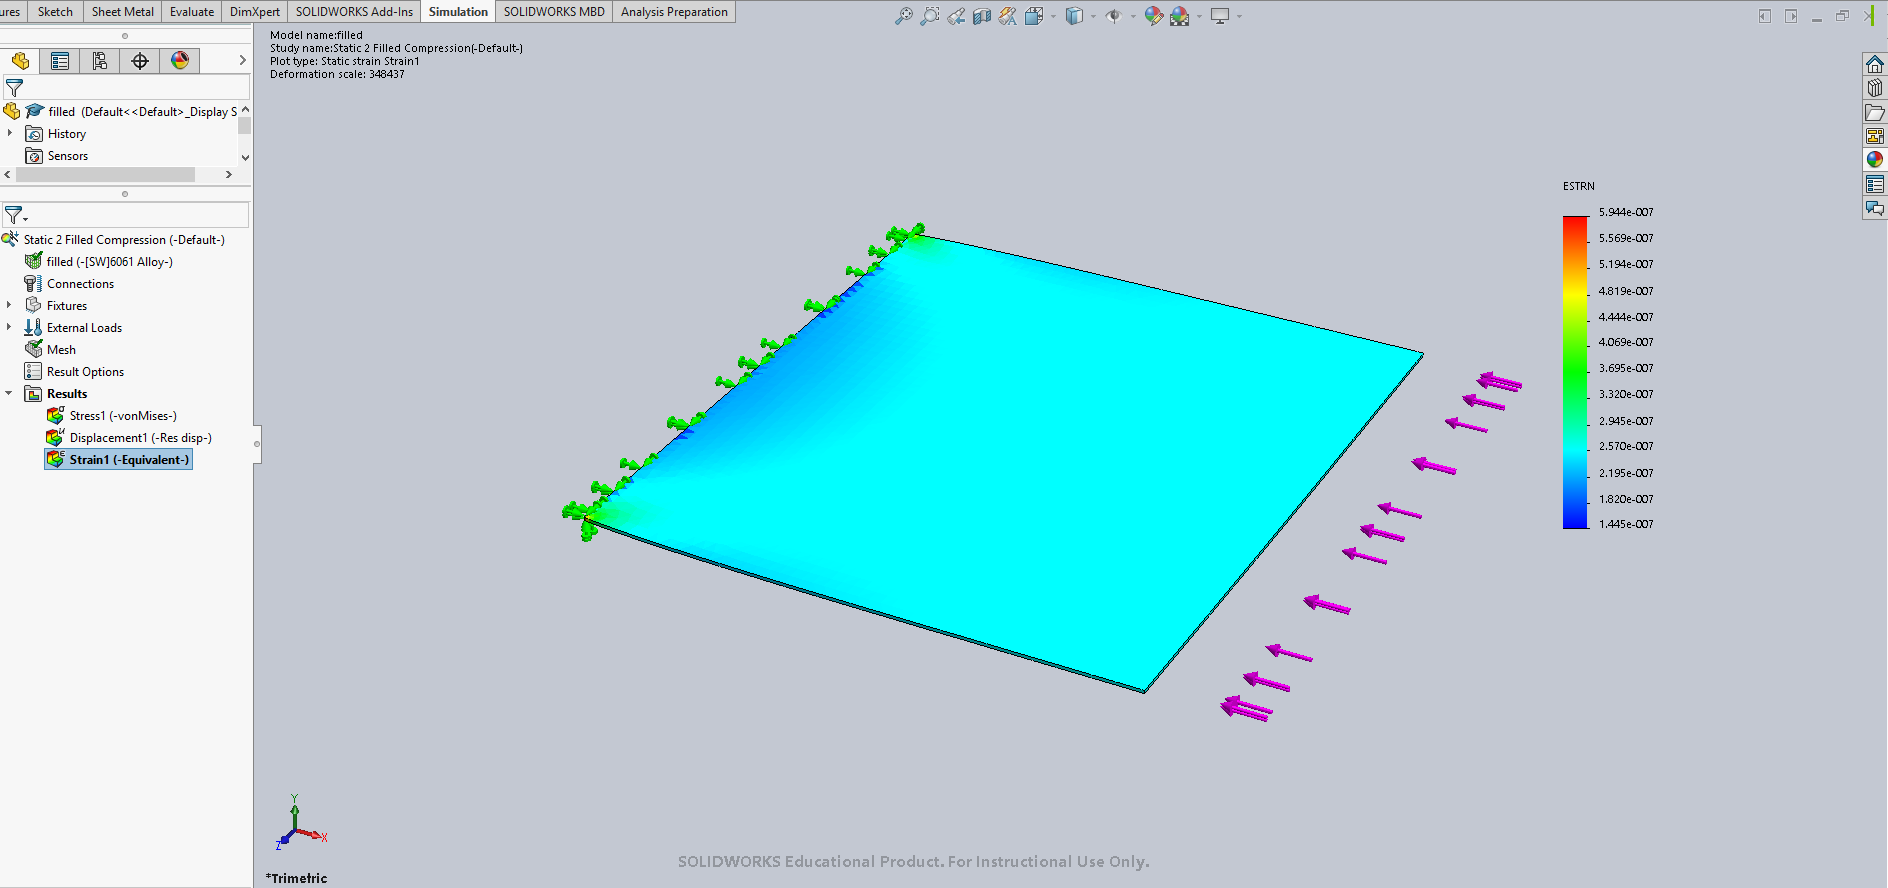
\includegraphics[width=0.8\linewidth]{./graphs/compression/filled-compression-strain}

\subsubsection{Square Compression Strain}
\label{ap:s-c-es}
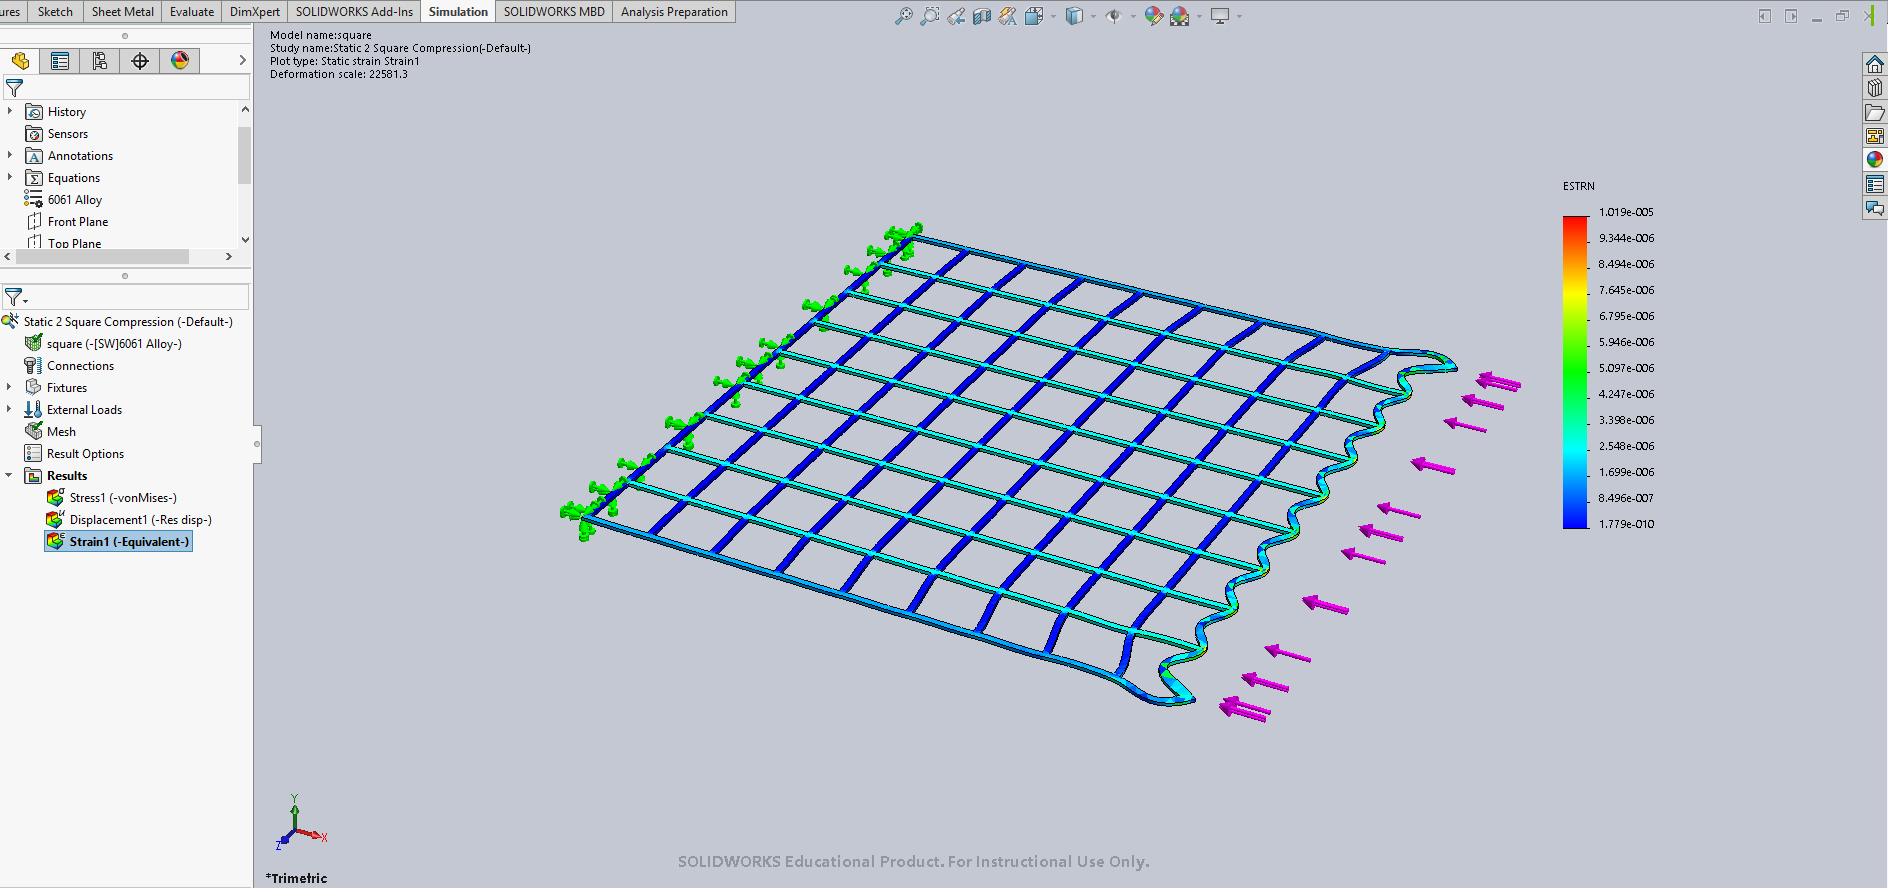
\includegraphics[width=0.8\linewidth]{./graphs/compression/square-compression-strain}

\subsubsection{Square Diamond Compression Strain}
\label{ap:sd-c-es}
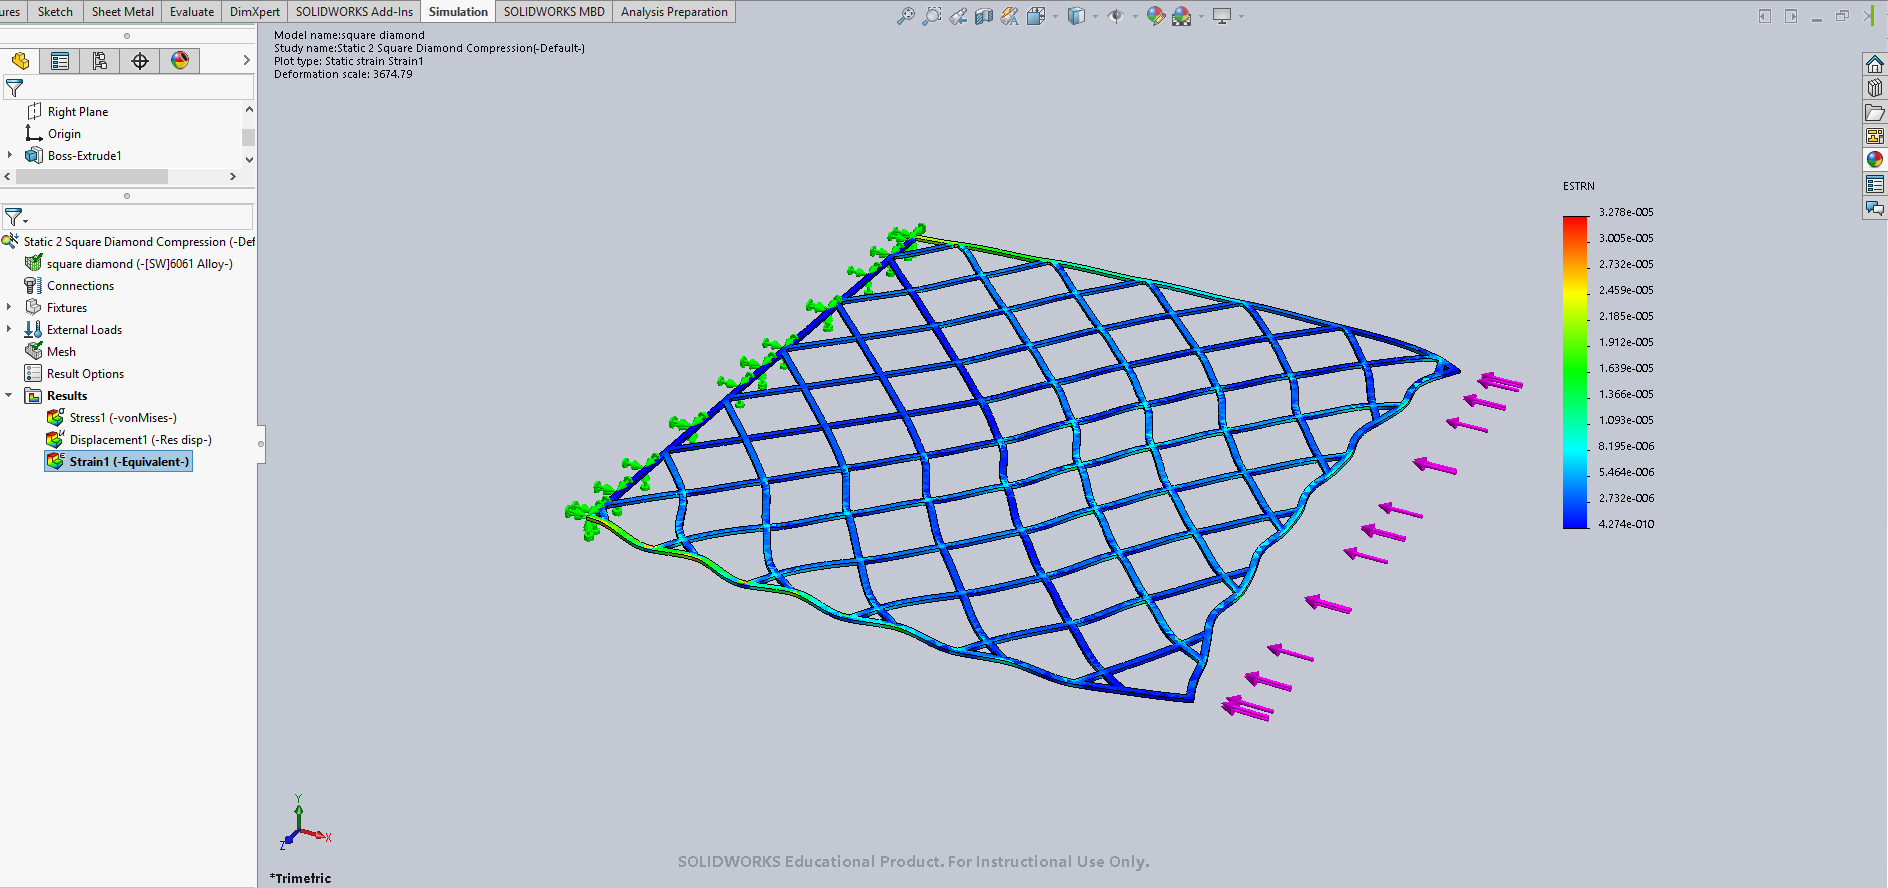
\includegraphics[width=0.8\linewidth]{./graphs/compression/square-diamond-compression-strain}

\subsubsection{Hex Compression Strain}
\label{ap:h-c-es}
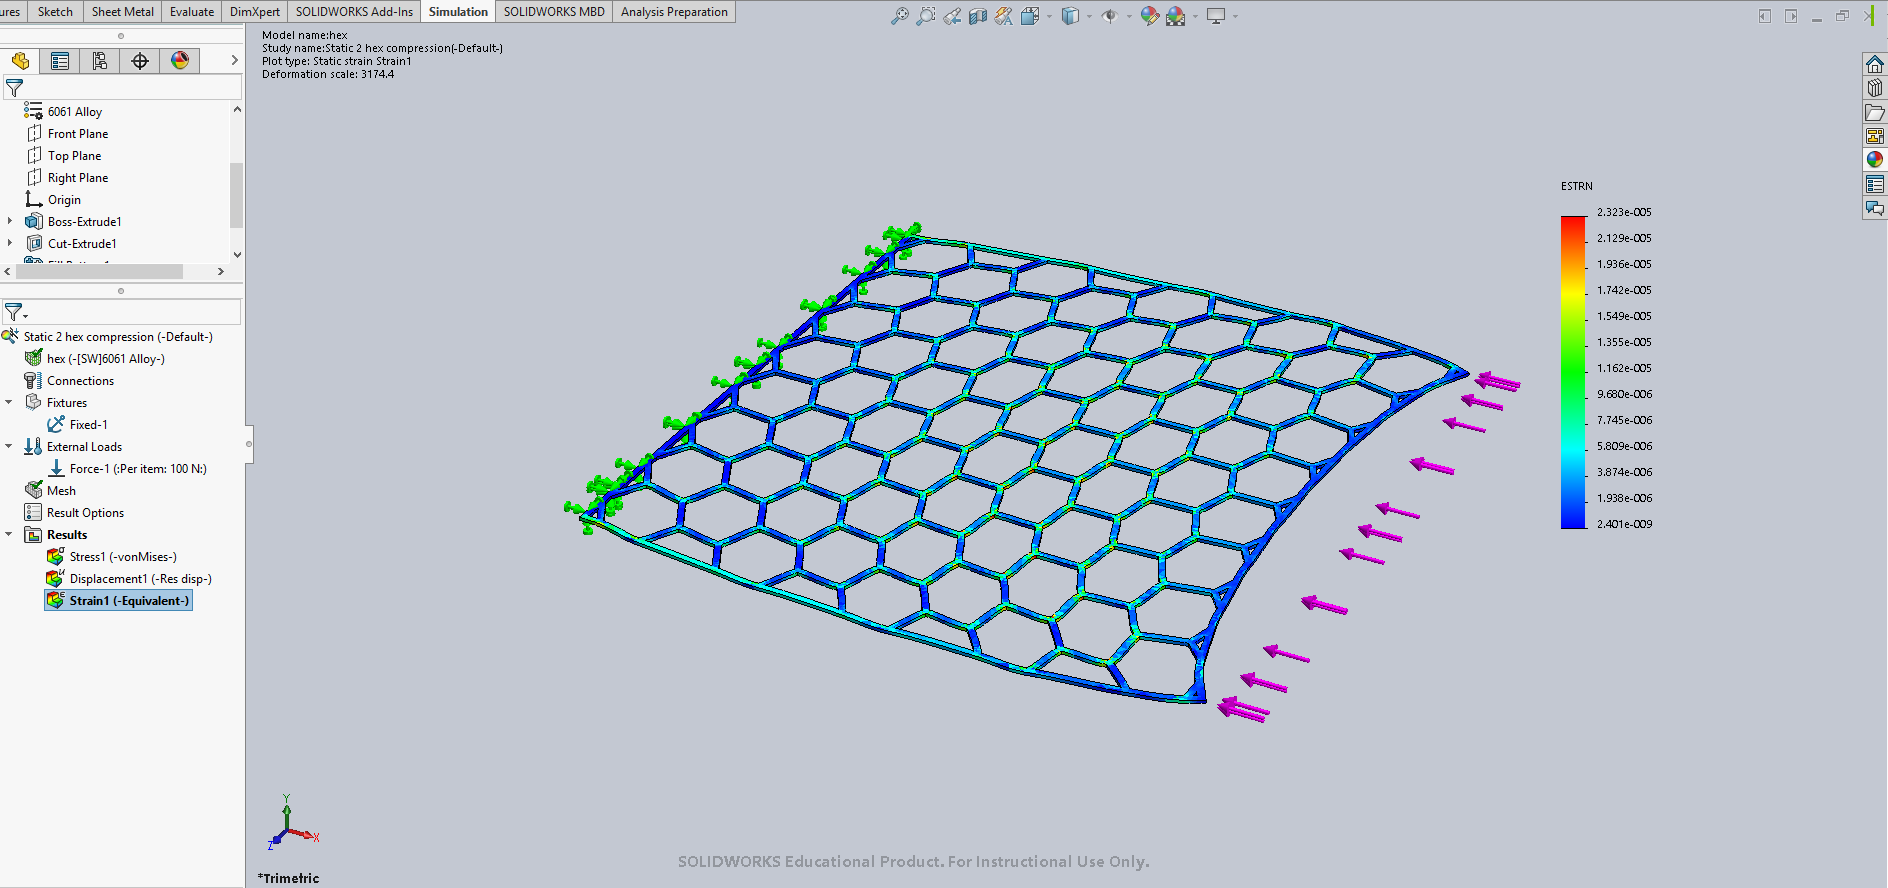
\includegraphics[width=0.8\linewidth]{./graphs/compression/hex-compression-strain}

\subsubsection{Hex Diamond Compression Strain}
\label{ap:hd-c-es}
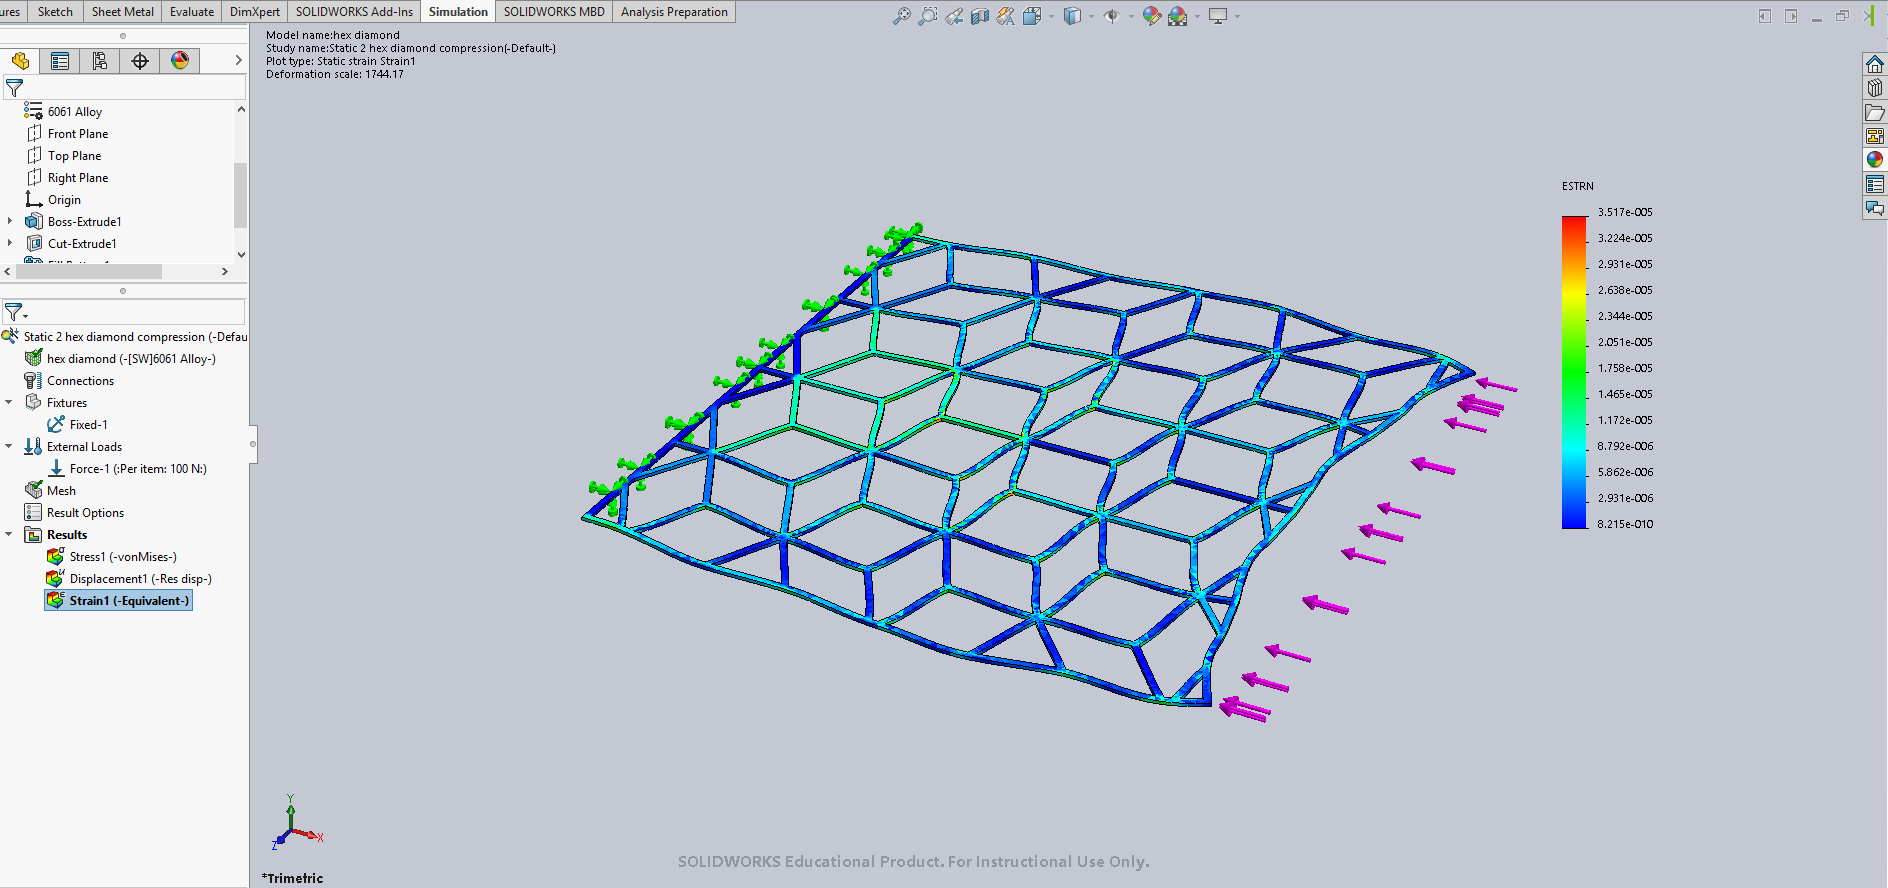
\includegraphics[width=0.8\linewidth]{./graphs/compression/hex-diamond-compression-strain}

\subsubsection{Triangle Compression Strain}
\label{ap:t-c-es}
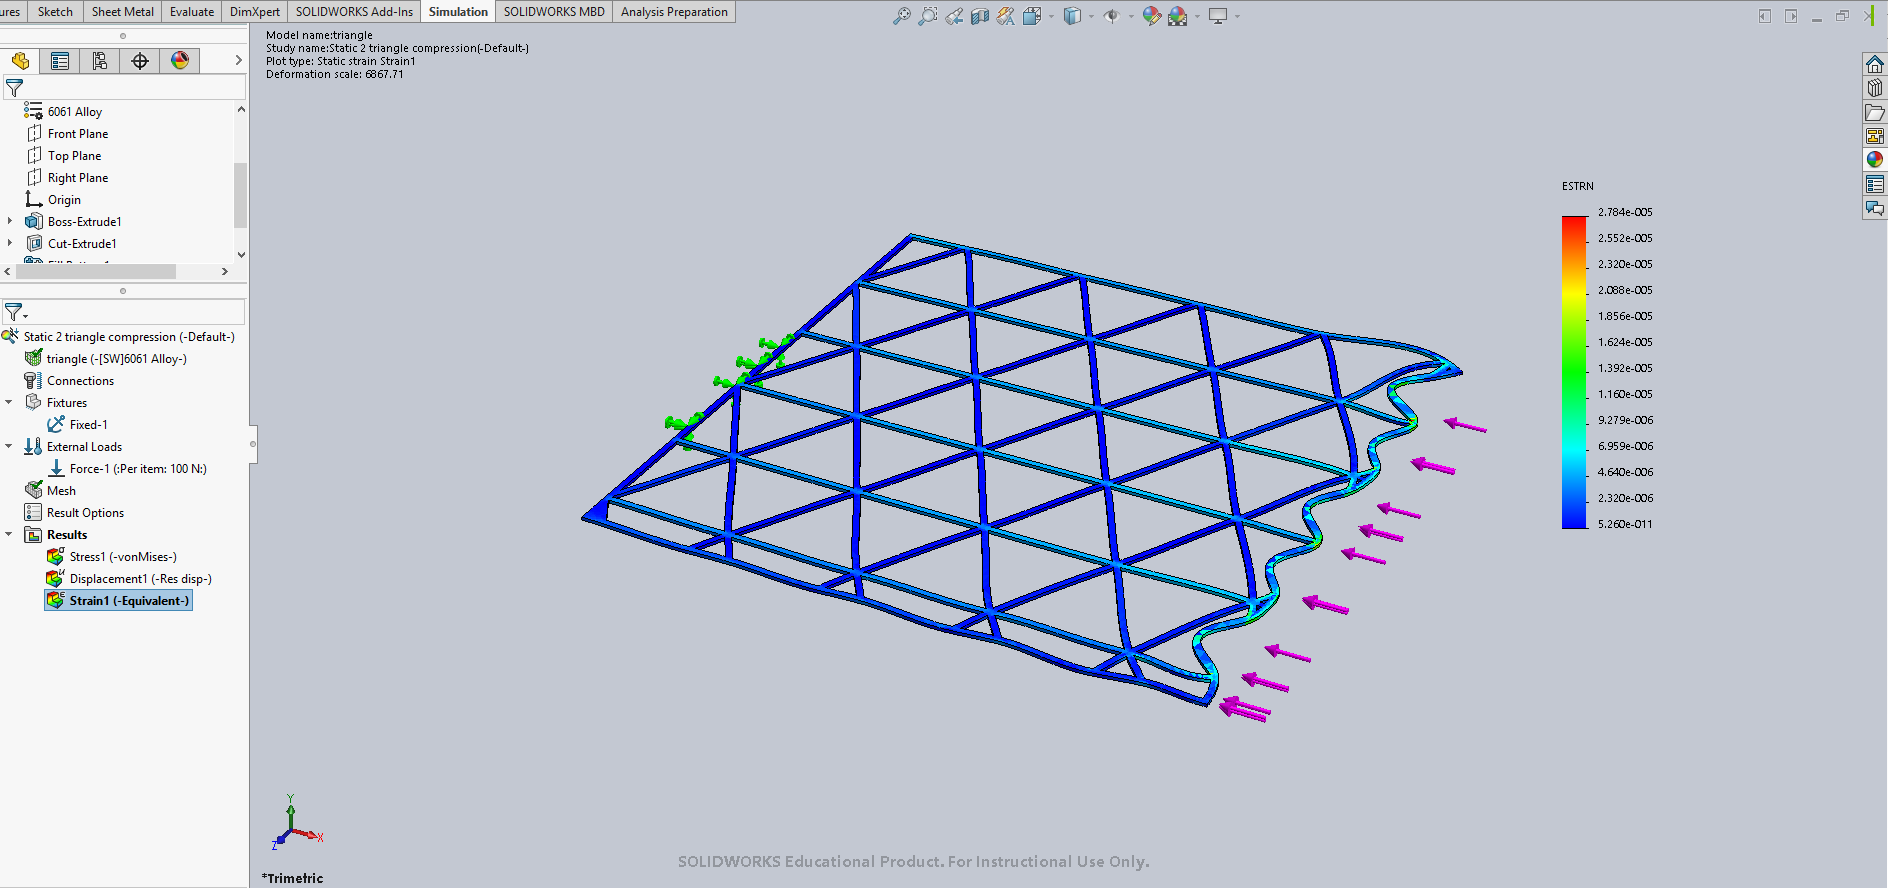
\includegraphics[width=0.8\linewidth]{./graphs/compression/triangle-compression-strain}


\subsection{Compression Displacement Graphs}
\label{ap:c-d}

\subsubsection{Filled Compression Displacement}
\label{ap:f-c-d}
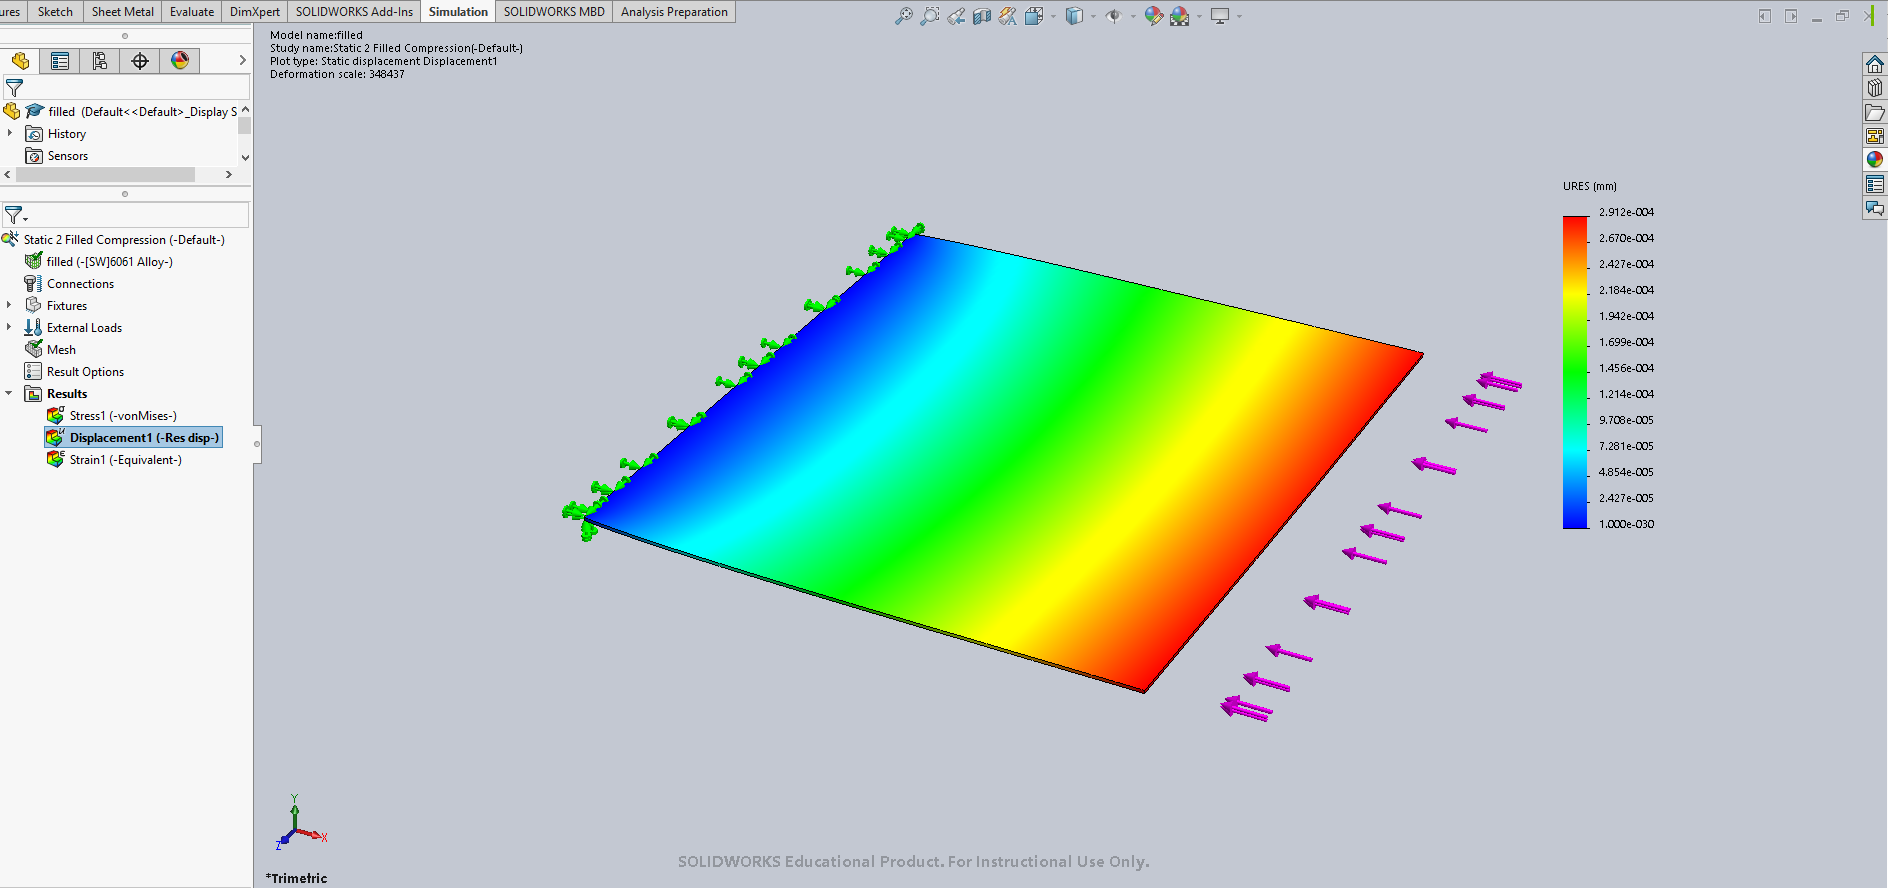
\includegraphics[width=0.8\linewidth]{./graphs/compression/filled-compression-displacement}

\subsubsection{Square Compression Displacement}
\label{ap:s-c-d}
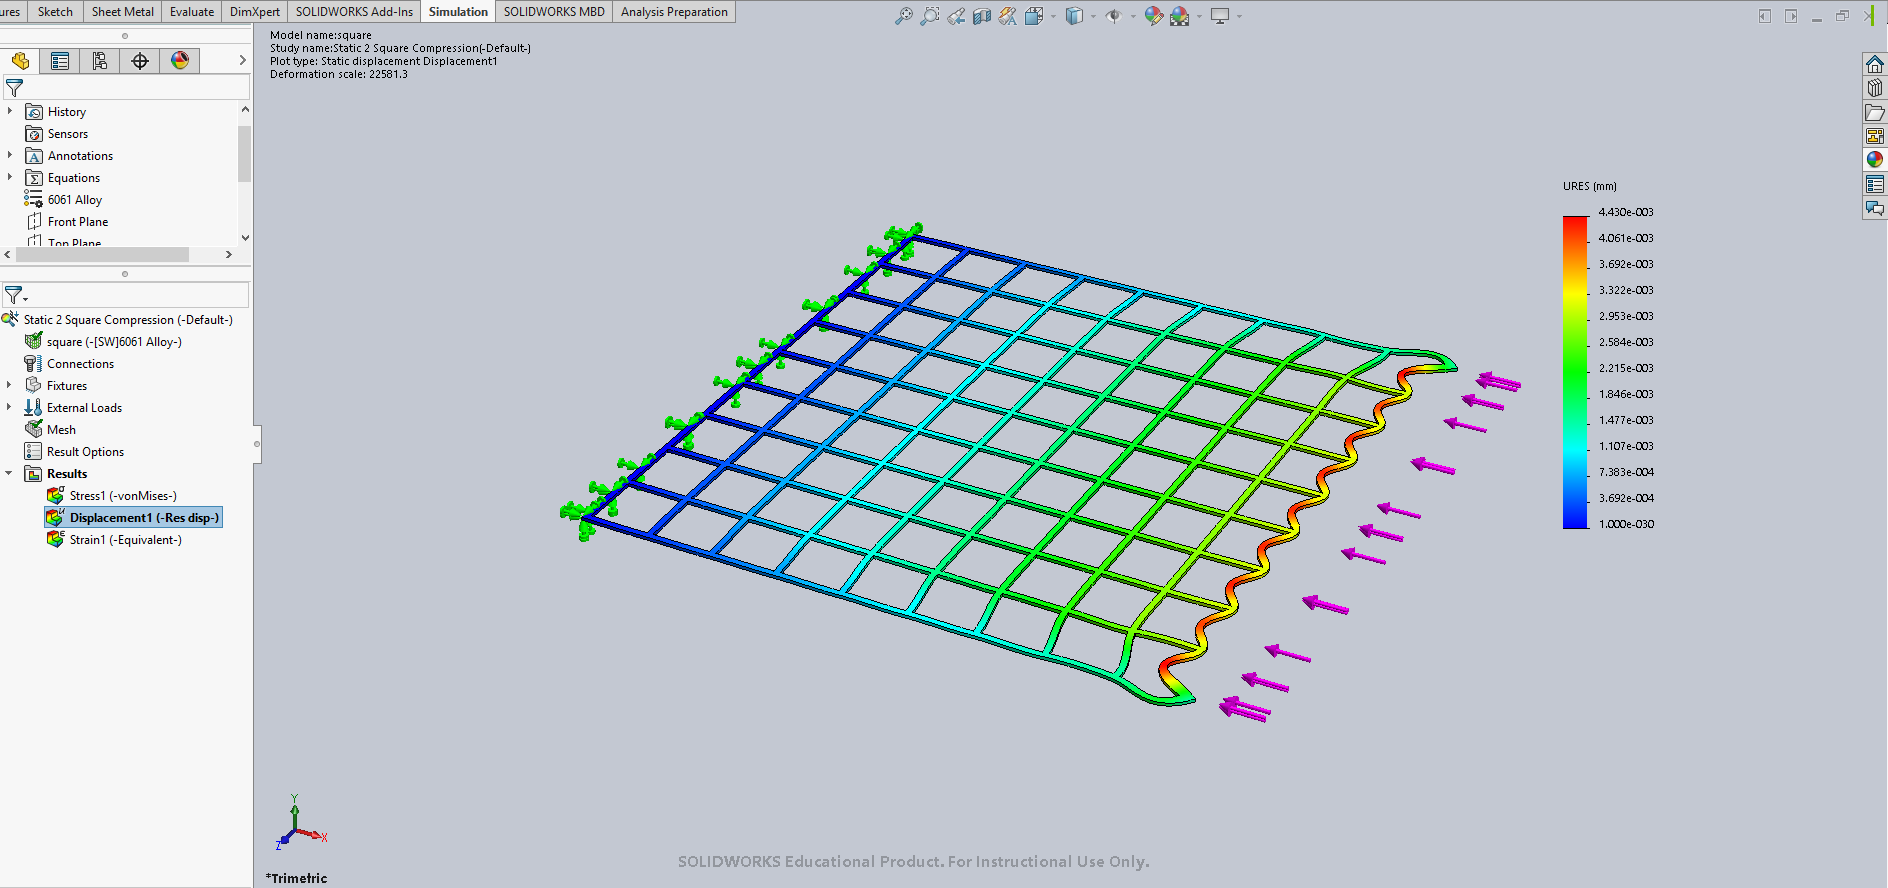
\includegraphics[width=0.8\linewidth]{./graphs/compression/square-compression-displacement}

\subsubsection{Square Diamond Compression Displacement}
\label{ap:sd-c-d}
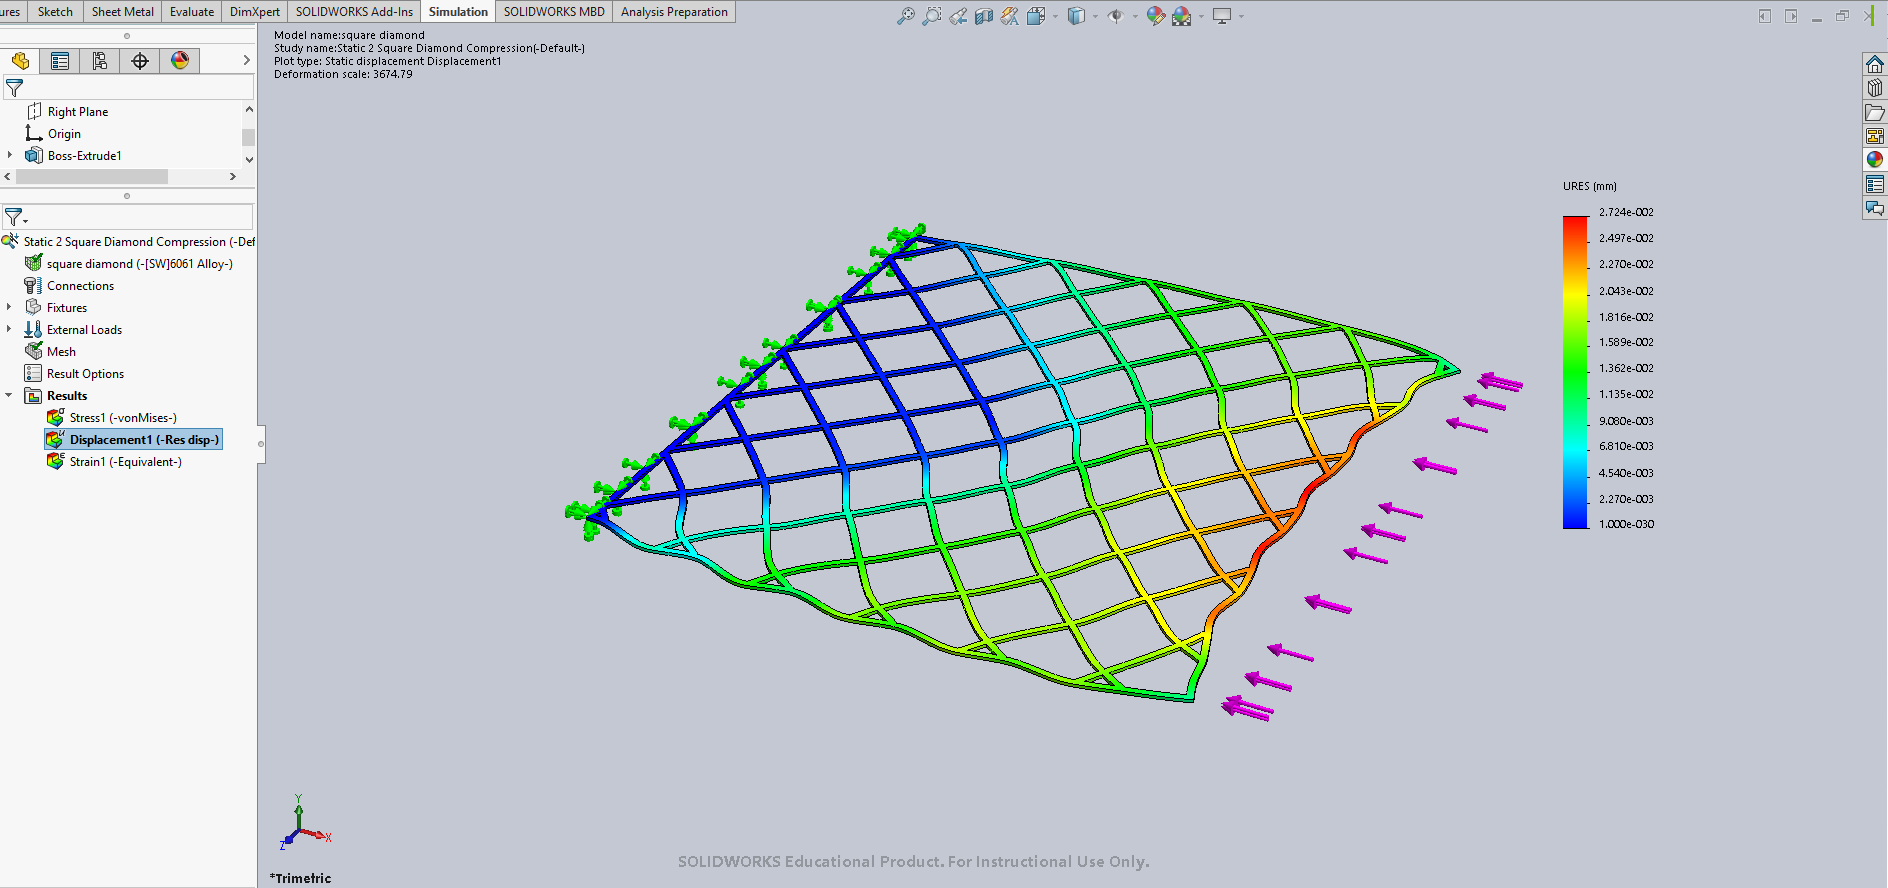
\includegraphics[width=0.8\linewidth]{./graphs/compression/square-diamond-compression-displacement}

\subsubsection{Hex Compression Displacement}
\label{ap:h-c-d}
\includegraphics[width=0.8\linewidth]{./graphs/compression/hex-compression-displacement}

\subsubsection{Hex Diamond Compression Displacement}
\label{ap:hd-c-d}
\includegraphics[width=0.8\linewidth]{./graphs/compression/hex-diamond-compression-displacement}

\subsubsection{Triangle Compression Displacement}
\label{ap:t-c-d}
\includegraphics[width=0.8\linewidth]{./graphs/compression/triangle-compression-displacement}



\section{Torsion Test Graphs}
\label{ap:to}



\subsection{Torsion Stress Graphs}
\label{ap:to-vm}


\subsubsection{Filled Torsion Stress}
\label{ap:f-to-vm}
\includegraphics[width=0.8\linewidth]{./graphs/torsion/filled-torsion-stress}

\subsubsection{Square Torsion Stress}
\label{ap:s-to-vm}
\includegraphics[width=0.8\linewidth]{./graphs/torsion/square-torsion-stress}

\subsubsection{Square Diamond Torsion Stress}
\label{ap:sd-to-vm}
\includegraphics[width=0.8\linewidth]{./graphs/torsion/square-diamond-torsion-stress}

\subsubsection{Hex Torsion Stress}
\label{ap:h-to-vm}
\includegraphics[width=0.8\linewidth]{./graphs/torsion/hex-torsion-stress}

\subsubsection{Hex Diamond Torsion Stress}
\label{ap:hd-to-vm}
\includegraphics[width=0.8\linewidth]{./graphs/torsion/hex-diamond-torsion-stress}

\subsubsection{Triangle Torsion Stress}
\label{ap:t-to-vm}
\includegraphics[width=0.8\linewidth]{./graphs/torsion/triangle-torsion-stress}


\subsection{Torsion Strain Graphs}
\label{ap:to-es}

\subsubsection{Filled Torsion Strain}
\label{ap:f-to-es}
\includegraphics[width=0.8\linewidth]{./graphs/torsion/filled-torsion-strain}

\subsubsection{Square Torsion Strain}
\label{ap:s-to-es}
\includegraphics[width=0.8\linewidth]{./graphs/torsion/square-torsion-strain}

\subsubsection{Square Diamond Torsion Strain}
\label{ap:sd-to-es}
\includegraphics[width=0.8\linewidth]{./graphs/torsion/square-diamond-torsion-strain}

\subsubsection{Hex Torsion Strain}
\label{ap:h-to-es}
\includegraphics[width=0.8\linewidth]{./graphs/torsion/hex-torsion-strain}

\subsubsection{Hex Diamond Torsion Strain}
\label{ap:hd-to-es}
\includegraphics[width=0.8\linewidth]{./graphs/torsion/hex-diamond-torsion-strain}

\subsubsection{Triangle Torsion Strain}
\label{ap:t-to-es}
\includegraphics[width=0.8\linewidth]{./graphs/torsion/triangle-torsion-strain}


\subsection{Torsion Displacement Graphs}
\label{ap:to-d}

\subsubsection{Filled Torsion Displacement}
\label{ap:f-to-d}
\includegraphics[width=0.8\linewidth]{./graphs/torsion/filled-torsion-displacement}

\subsubsection{Square Torsion Displacement}
\label{ap:s-to-d}
\includegraphics[width=0.8\linewidth]{./graphs/torsion/square-torsion-displacement}

\subsubsection{Square Diamond Torsion Displacement}
\label{ap:sd-to-d}
\includegraphics[width=0.8\linewidth]{./graphs/torsion/square-diamond-torsion-displacement}

\subsubsection{Hex Torsion Displacement}
\label{ap:h-to-d}
\includegraphics[width=0.8\linewidth]{./graphs/torsion/hex-torsion-displacement}

\subsubsection{Hex Diamond Torsion Displacement}
\label{ap:hd-to-d}
\includegraphics[width=0.8\linewidth]{./graphs/torsion/hex-diamond-torsion-displacement}

\subsubsection{Triangle Torsion Displacement}
\label{ap:t-to-d}
\includegraphics[width=0.8\linewidth]{./graphs/torsion/triangle-torsion-displacement}



\section{Simulation Animations and Data}
\label{ap:data}

All animations and .csv data files are found at the \href{https://github.com/tynanpurdy/physics-ia/tree/master/data}{project GitHub repository}.

\url{https://github.com/tynanpurdy/physics-ia/tree/master/data}

\end{singlespace}
\end{document}